% **************************************************************************************************************
% A Classic Thesis Style
% An Homage to The Elements of Typographic Style
%
% Copyright (C) 2025 André Miede and Ivo Pletikosić
%
% If you like the style then I would appreciate a postcard. My address
% can be found in the file ClassicThesis.pdf. A collection of the
% postcards I received so far is available online at
% http://postcards.miede.de
%
% License:
% This program is free software; you can redistribute it and/or modify
% it under the terms of the GNU General Public License as published by
% the Free Software Foundation; either version 2 of the License, or
% (at your option) any later version.
%
% This program is distributed in the hope that it will be useful,
% but WITHOUT ANY WARRANTY; without even the implied warranty of
% MERCHANTABILITY or FITNESS FOR A PARTICULAR PURPOSE.  See the
% GNU General Public License for more details.
%
% You should have received a copy of the GNU General Public License
% along with this program; see the file COPYING.  If not, write to
% the Free Software Foundation, Inc., 59 Temple Place - Suite 330,
% Boston, MA 02111-1307, USA.
%
% PLEASE SEE ALSO THE AUTHORS' NOTE REGARDING THIS LICENSE
% IN THE DOCUMENTATION (ClassicThesis.pdf --> Chapter 1 / Chapter01.tex)
% **************************************************************************************************************
\RequirePackage{silence} % :-\
    \WarningFilter{scrreprt}{Usage of package `titlesec'}
    %\WarningFilter{scrreprt}{Activating an ugly workaround}
    \WarningFilter{titlesec}{Non standard sectioning command detected}
\documentclass[ twoside,openright,titlepage,numbers=noenddot,%1headlines,
                headinclude,footinclude,cleardoublepage=empty,abstract=on,
                BCOR=5mm,paper=a4,fontsize=11pt
                ]{scrreprt}

%********************************************************************
% Note: Make all your adjustments in here
%*******************************************************
% ****************************************************************************************************
% classicthesis-config.tex
% formerly known as loadpackages.sty, classicthesis-ldpkg.sty, and classicthesis-preamble.sty
% Use it at the beginning of your ClassicThesis.tex, or as a LaTeX Preamble
% in your ClassicThesis.{tex,lyx} with % ****************************************************************************************************
% classicthesis-config.tex
% formerly known as loadpackages.sty, classicthesis-ldpkg.sty, and classicthesis-preamble.sty
% Use it at the beginning of your ClassicThesis.tex, or as a LaTeX Preamble
% in your ClassicThesis.{tex,lyx} with % ****************************************************************************************************
% classicthesis-config.tex
% formerly known as loadpackages.sty, classicthesis-ldpkg.sty, and classicthesis-preamble.sty
% Use it at the beginning of your ClassicThesis.tex, or as a LaTeX Preamble
% in your ClassicThesis.{tex,lyx} with \input{classicthesis-config}
% ****************************************************************************************************
% If you like the classicthesis, then I would appreciate a postcard.
% My address can be found in the file ClassicThesis.pdf. A collection
% of the postcards I received so far is available online at
% http://postcards.miede.de
% ****************************************************************************************************


% ****************************************************************************************************
% 0. Set the encoding of your files. UTF-8 is the only sensible encoding nowadays. If you can't read
% äöüßáéçèê∂åëæƒÏ€ then change the encoding setting in your editor, not the line below. If your editor
% does not support utf8 use another editor!
% ****************************************************************************************************
\PassOptionsToPackage{utf8}{inputenc}
  \usepackage{inputenc}

\PassOptionsToPackage{T1}{fontenc} % T2A for cyrillics
  \usepackage{fontenc}


% ****************************************************************************************************
% 1. Configure classicthesis for your needs here, e.g., remove "drafting" below
% in order to deactivate the time-stamp on the pages
% (see ClassicThesis.pdf for more information):
% ****************************************************************************************************
\PassOptionsToPackage{
  drafting=true,    % print version information on the bottom of the pages
  tocaligned=false, % the left column of the toc will be aligned (no indentation)
  dottedtoc=false,  % page numbers in ToC flushed right
  eulerchapternumbers=false, % use AMS Euler for chapter font (otherwise Palatino)
  floatperchapter=true,     % numbering per chapter for all floats (i.e., Figure 1.1)
  eulermath=false,  % use awesome Euler fonts for mathematical formulae (only with pdfLaTeX)
  beramono=true,    % toggle a nice monospaced font (w/ bold)
  palatino=true,    % deactivate standard font for loading another one, see the last section at the end of this file for suggestions
  %linedheaders=true, % obsolete / available for backwards compatibility
  style=classicthesis % classicthesis, arsclassica, linedheaders, plain
}{classicthesis}

% ****************************************************************************************************
% 2. Personal data and user ad-hoc commands (insert your own data here)
% ****************************************************************************************************
\newcommand{\myTitle}{Task Allocation and Stop Optimization for Autonomous Weeding\xspace}
\newcommand{\mySubtitle}{A Multi-Tool Allocation Approach for Optimized Weed Removal in Autonomous Agriculture\xspace}
\newcommand{\myDegree}{Master of Science in Intelligent Field Robotic Systems (MSc)\xspace}
\newcommand{\myName}{David Razhiel Ceres Arroyo\xspace}
\newcommand{\myProf}{Tamara Petrović\xspace}
\newcommand{\myOtherProf}{Put name here\xspace}
\newcommand{\mySupervisor}{Tamara Petrović\xspace}
\newcommand{\myFaculty}{Faculty of Electrical Engineering and Computing\xspace}
\newcommand{\myDepartment}{Put data here\xspace}
\newcommand{\myUni}{University of Zagreb\xspace}
\newcommand{\myLocation}{Zagreb, Croatia\xspace}
\newcommand{\myTime}{June 2025\xspace}
\newcommand{\myVersion}{\classicthesis}

% ********************************************************************
% Setup, finetuning, and useful commands
% ********************************************************************
\providecommand{\mLyX}{L\kern-.1667em\lower.25em\hbox{Y}\kern-.125emX\@}
\newcommand{\ie}{i.\,e.}
\newcommand{\Ie}{I.\,e.}
\newcommand{\eg}{e.\,g.}
\newcommand{\Eg}{E.\,g.}
% ****************************************************************************************************


% ****************************************************************************************************
% 3. Loading some handy packages
% ****************************************************************************************************
% ********************************************************************
% Packages with options that might require adjustments
% ********************************************************************
\PassOptionsToPackage{ngerman,american}{babel} % change this to your language(s), main language last
% Spanish languages need extra options in order to work with this template
%\PassOptionsToPackage{spanish,es-lcroman}{babel}
    \usepackage{babel}

\usepackage{csquotes}
\PassOptionsToPackage{%
  %backend=biber,bibencoding=utf8, %instead of bibtex
  backend=bibtex8,bibencoding=auto,% ascii
  language=auto,%
  style=numeric-comp,%
  %style=authoryear-comp, % Author 1999, 2010
  %bibstyle=authoryear,dashed=false, % dashed: substitute rep. author with ---
  sorting=nyt, % name, year, title
  maxbibnames=10, % default: 3, et al.
  %backref=true,%
  natbib=true % natbib compatibility mode (\citep and \citet still work)
}{biblatex}
    \usepackage{biblatex}

\PassOptionsToPackage{fleqn}{amsmath}       % math environments and more by the AMS
  \usepackage{amsmath}

% ********************************************************************
% General useful packages
% ********************************************************************
\usepackage{graphicx} %
\usepackage{scrhack} % fix warnings when using KOMA with listings package
\usepackage{xspace} % to get the spacing after macros right
\PassOptionsToPackage{printonlyused,smaller}{acronym}
  \usepackage{acronym} % nice macros for handling all acronyms in the thesis
  %\renewcommand{\bflabel}[1]{{#1}\hfill} % fix the list of acronyms --> no longer working
  %\renewcommand*{\acsfont}[1]{\textsc{#1}}
  %\renewcommand*{\aclabelfont}[1]{\acsfont{#1}}
  %\def\bflabel#1{{#1\hfill}}
  \def\bflabel#1{{\acsfont{#1}\hfill}}
  \def\aclabelfont#1{\acsfont{#1}}
% ****************************************************************************************************
%\usepackage{pgfplots} % External TikZ/PGF support (thanks to Andreas Nautsch)
%\usetikzlibrary{external}
%\tikzexternalize[mode=list and make, prefix=ext-tikz/]
% ****************************************************************************************************


% ****************************************************************************************************
% 4. Setup floats: tables, (sub)figures, and captions
% ****************************************************************************************************
\usepackage{tabularx} % better tables
  \setlength{\extrarowheight}{3pt} % increase table row height
\newcommand{\tableheadline}[1]{\multicolumn{1}{l}{\spacedlowsmallcaps{#1}}}
\newcommand{\myfloatalign}{\centering} % to be used with each float for alignment
\usepackage{subfig}
% ****************************************************************************************************


% ****************************************************************************************************
% 5. Setup code listings
% ****************************************************************************************************
\usepackage{listings}
%\lstset{emph={trueIndex,root},emphstyle=\color{BlueViolet}}%\underbar} % for special keywords
\lstset{language=[LaTeX]Tex,%C++,
  morekeywords={PassOptionsToPackage,selectlanguage},
  keywordstyle=\color{RoyalBlue},%\bfseries,
  basicstyle=\small\ttfamily,
  %identifierstyle=\color{NavyBlue},
  commentstyle=\color{Green}\ttfamily,
  stringstyle=\rmfamily,
  numbers=none,%left,%
  numberstyle=\scriptsize,%\tiny
  stepnumber=5,
  numbersep=8pt,
  showstringspaces=false,
  breaklines=true,
  %frameround=ftff,
  %frame=single,
  belowcaptionskip=.75\baselineskip
  %frame=L
}

% For YAML files
\lstdefinelanguage{yaml}{
  keywords={true,false},
  keywordstyle=\color{RoyalBlue}\bfseries,
  basicstyle=\ttfamily\small,
  sensitive=true,
  comment=[l]{\#},
  morecomment=[s]{/*}{*/},
  commentstyle=\color{Green}\ttfamily,
  stringstyle=\color{YamlString},
  showstringspaces=false,
  moredelim=[l][\color{gray}]{-},
  identifierstyle=\color{YamlKeyword}\bfseries,
  emph={clustered,uniform,x},
  emphstyle=\color{YamlString},
  breaklines=true,
  belowcaptionskip=.75\baselineskip,
}
% ****************************************************************************************************


% ****************************************************************************************************
% 6. Last calls before the bar closes
% ****************************************************************************************************
% ********************************************************************
% Her Majesty herself
% ********************************************************************
\PassOptionsToPackage{hyperfootnotes=false}{hyperref}
\usepackage{classicthesis}


% ********************************************************************
% Fine-tune hyperreferences (hyperref should be called last)
% ********************************************************************
\hypersetup{%
  %draft, % hyperref's draft mode, for printing see below
  colorlinks=true, linktocpage=true, pdfstartpage=3, pdfstartview=FitV,%
  % uncomment the following line if you want to have black links (e.g., for printing)
  %colorlinks=false, linktocpage=false, pdfstartpage=3, pdfstartview=FitV, pdfborder={0 0 0},%
  breaklinks=true, pageanchor=true,%
  pdfpagemode=UseNone, %
  % pdfpagemode=UseOutlines,%
  plainpages=false, bookmarksnumbered, bookmarksopen=true, bookmarksopenlevel=1,%
  hypertexnames=true, pdfhighlight=/O,%nesting=true,%frenchlinks,%
  urlcolor=CTurl, linkcolor=CTlink, citecolor=CTcitation, %pagecolor=RoyalBlue,%
  %urlcolor=Black, linkcolor=Black, citecolor=Black, %pagecolor=Black,%
  pdftitle={\myTitle},%
  pdfauthor={\textcopyright\ \myName, \myUni, \myFaculty},%
  pdfsubject={},%
  pdfkeywords={},%
  pdfcreator={pdfLaTeX},%
  pdfproducer={LaTeX with hyperref and classicthesis}%
}


% ********************************************************************
% Setup autoreferences (hyperref and babel)
% ********************************************************************
% There are some issues regarding autorefnames
% http://www.tex.ac.uk/cgi-bin/texfaq2html?label=latexwords
% you have to redefine the macros for the
% language you use, e.g., american, ngerman
% (as chosen when loading babel/AtBeginDocument)
% ********************************************************************
 \makeatletter
 \@ifpackageloaded{babel}%
   {%
     \addto\extrasamerican{%
       \renewcommand*{\figureautorefname}{Figure}%
       \renewcommand*{\tableautorefname}{Table}%
       \renewcommand*{\partautorefname}{Part}%
       \renewcommand*{\chapterautorefname}{Chapter}%
       \renewcommand*{\sectionautorefname}{Section}%
       \renewcommand*{\subsectionautorefname}{Section}%
       \renewcommand*{\subsubsectionautorefname}{Section}%
     }%
     \addto\extrasngerman{%
       \renewcommand*{\paragraphautorefname}{Absatz}%
       \renewcommand*{\subparagraphautorefname}{Unterabsatz}%
       \renewcommand*{\footnoteautorefname}{Fu\"snote}%
       \renewcommand*{\FancyVerbLineautorefname}{Zeile}%
       \renewcommand*{\theoremautorefname}{Theorem}%
       \renewcommand*{\appendixautorefname}{Anhang}%
       \renewcommand*{\equationautorefname}{Gleichung}%
       \renewcommand*{\itemautorefname}{Punkt}%
     }%
       % Fix to getting autorefs for subfigures right (thanks to Belinda Vogt for changing the definition)
       \providecommand{\subfigureautorefname}{\figureautorefname}%
     }{\relax}
 \makeatother

% (Better) alternative to \autoref is \cref via the cleveref package
%\usepackage{cleveref}
%\crefformat{part}{Part #2\MakeUppercase{#1}#3}


% ********************************************************************
% Development Stuff
% ********************************************************************
\listfiles
%\PassOptionsToPackage{l2tabu,orthodox,abort}{nag}
%  \usepackage{nag}
%\PassOptionsToPackage{warning, all}{onlyamsmath}
%  \usepackage{onlyamsmath}


% ****************************************************************************************************
% 7. Further adjustments (experimental)
% ****************************************************************************************************
% ********************************************************************
% Changing the text area
% ********************************************************************
%\areaset[current]{312pt}{761pt} % 686 (factor 2.2) + 33 head + 42 head \the\footskip
%\setlength{\marginparwidth}{7em}%
%\setlength{\marginparsep}{2em}%

% ********************************************************************
% Using different fonts
% ********************************************************************
%\usepackage[oldstylenums]{kpfonts} % oldstyle notextcomp
% \usepackage[osf]{libertine}
%\usepackage[light,condensed,math]{iwona}
%\renewcommand{\sfdefault}{iwona}
%\usepackage{lmodern} % <-- no osf support :-(
%\usepackage{cfr-lm} %
%\usepackage[urw-garamond]{mathdesign} <-- no osf support :-(
%\usepackage[default,osfigures]{opensans} % scale=0.95
%\usepackage[sfdefault]{FiraSans}
% \usepackage[opticals,mathlf]{MinionPro} % onlytext
% ********************************************************************
%\usepackage[largesc,osf]{newpxtext}
%\linespread{1.05} % a bit more for Palatino
% Used to fix these:
% https://bitbucket.org/amiede/classicthesis/issues/139/italics-in-pallatino-capitals-chapter
% https://bitbucket.org/amiede/classicthesis/issues/45/problema-testatine-su-classicthesis-style
% ********************************************************************
% ****************************************************************************************************
% David's Packages
\usepackage{multirow} % For merging cells
\usepackage{float} % Enables use of [H] when placing imgs
\usepackage{lipsum}
\usepackage{algorithm}
\usepackage{algorithmic}
% ********************************************************************
% ****************************************************************************************************
% If you like the classicthesis, then I would appreciate a postcard.
% My address can be found in the file ClassicThesis.pdf. A collection
% of the postcards I received so far is available online at
% http://postcards.miede.de
% ****************************************************************************************************


% ****************************************************************************************************
% 0. Set the encoding of your files. UTF-8 is the only sensible encoding nowadays. If you can't read
% äöüßáéçèê∂åëæƒÏ€ then change the encoding setting in your editor, not the line below. If your editor
% does not support utf8 use another editor!
% ****************************************************************************************************
\PassOptionsToPackage{utf8}{inputenc}
  \usepackage{inputenc}

\PassOptionsToPackage{T1}{fontenc} % T2A for cyrillics
  \usepackage{fontenc}


% ****************************************************************************************************
% 1. Configure classicthesis for your needs here, e.g., remove "drafting" below
% in order to deactivate the time-stamp on the pages
% (see ClassicThesis.pdf for more information):
% ****************************************************************************************************
\PassOptionsToPackage{
  drafting=true,    % print version information on the bottom of the pages
  tocaligned=false, % the left column of the toc will be aligned (no indentation)
  dottedtoc=false,  % page numbers in ToC flushed right
  eulerchapternumbers=false, % use AMS Euler for chapter font (otherwise Palatino)
  floatperchapter=true,     % numbering per chapter for all floats (i.e., Figure 1.1)
  eulermath=false,  % use awesome Euler fonts for mathematical formulae (only with pdfLaTeX)
  beramono=true,    % toggle a nice monospaced font (w/ bold)
  palatino=true,    % deactivate standard font for loading another one, see the last section at the end of this file for suggestions
  %linedheaders=true, % obsolete / available for backwards compatibility
  style=classicthesis % classicthesis, arsclassica, linedheaders, plain
}{classicthesis}

% ****************************************************************************************************
% 2. Personal data and user ad-hoc commands (insert your own data here)
% ****************************************************************************************************
\newcommand{\myTitle}{Task Allocation and Stop Optimization for Autonomous Weeding\xspace}
\newcommand{\mySubtitle}{A Multi-Tool Allocation Approach for Optimized Weed Removal in Autonomous Agriculture\xspace}
\newcommand{\myDegree}{Master of Science in Intelligent Field Robotic Systems (MSc)\xspace}
\newcommand{\myName}{David Razhiel Ceres Arroyo\xspace}
\newcommand{\myProf}{Tamara Petrović\xspace}
\newcommand{\myOtherProf}{Put name here\xspace}
\newcommand{\mySupervisor}{Tamara Petrović\xspace}
\newcommand{\myFaculty}{Faculty of Electrical Engineering and Computing\xspace}
\newcommand{\myDepartment}{Put data here\xspace}
\newcommand{\myUni}{University of Zagreb\xspace}
\newcommand{\myLocation}{Zagreb, Croatia\xspace}
\newcommand{\myTime}{June 2025\xspace}
\newcommand{\myVersion}{\classicthesis}

% ********************************************************************
% Setup, finetuning, and useful commands
% ********************************************************************
\providecommand{\mLyX}{L\kern-.1667em\lower.25em\hbox{Y}\kern-.125emX\@}
\newcommand{\ie}{i.\,e.}
\newcommand{\Ie}{I.\,e.}
\newcommand{\eg}{e.\,g.}
\newcommand{\Eg}{E.\,g.}
% ****************************************************************************************************


% ****************************************************************************************************
% 3. Loading some handy packages
% ****************************************************************************************************
% ********************************************************************
% Packages with options that might require adjustments
% ********************************************************************
\PassOptionsToPackage{ngerman,american}{babel} % change this to your language(s), main language last
% Spanish languages need extra options in order to work with this template
%\PassOptionsToPackage{spanish,es-lcroman}{babel}
    \usepackage{babel}

\usepackage{csquotes}
\PassOptionsToPackage{%
  %backend=biber,bibencoding=utf8, %instead of bibtex
  backend=bibtex8,bibencoding=auto,% ascii
  language=auto,%
  style=numeric-comp,%
  %style=authoryear-comp, % Author 1999, 2010
  %bibstyle=authoryear,dashed=false, % dashed: substitute rep. author with ---
  sorting=nyt, % name, year, title
  maxbibnames=10, % default: 3, et al.
  %backref=true,%
  natbib=true % natbib compatibility mode (\citep and \citet still work)
}{biblatex}
    \usepackage{biblatex}

\PassOptionsToPackage{fleqn}{amsmath}       % math environments and more by the AMS
  \usepackage{amsmath}

% ********************************************************************
% General useful packages
% ********************************************************************
\usepackage{graphicx} %
\usepackage{scrhack} % fix warnings when using KOMA with listings package
\usepackage{xspace} % to get the spacing after macros right
\PassOptionsToPackage{printonlyused,smaller}{acronym}
  \usepackage{acronym} % nice macros for handling all acronyms in the thesis
  %\renewcommand{\bflabel}[1]{{#1}\hfill} % fix the list of acronyms --> no longer working
  %\renewcommand*{\acsfont}[1]{\textsc{#1}}
  %\renewcommand*{\aclabelfont}[1]{\acsfont{#1}}
  %\def\bflabel#1{{#1\hfill}}
  \def\bflabel#1{{\acsfont{#1}\hfill}}
  \def\aclabelfont#1{\acsfont{#1}}
% ****************************************************************************************************
%\usepackage{pgfplots} % External TikZ/PGF support (thanks to Andreas Nautsch)
%\usetikzlibrary{external}
%\tikzexternalize[mode=list and make, prefix=ext-tikz/]
% ****************************************************************************************************


% ****************************************************************************************************
% 4. Setup floats: tables, (sub)figures, and captions
% ****************************************************************************************************
\usepackage{tabularx} % better tables
  \setlength{\extrarowheight}{3pt} % increase table row height
\newcommand{\tableheadline}[1]{\multicolumn{1}{l}{\spacedlowsmallcaps{#1}}}
\newcommand{\myfloatalign}{\centering} % to be used with each float for alignment
\usepackage{subfig}
% ****************************************************************************************************


% ****************************************************************************************************
% 5. Setup code listings
% ****************************************************************************************************
\usepackage{listings}
%\lstset{emph={trueIndex,root},emphstyle=\color{BlueViolet}}%\underbar} % for special keywords
\lstset{language=[LaTeX]Tex,%C++,
  morekeywords={PassOptionsToPackage,selectlanguage},
  keywordstyle=\color{RoyalBlue},%\bfseries,
  basicstyle=\small\ttfamily,
  %identifierstyle=\color{NavyBlue},
  commentstyle=\color{Green}\ttfamily,
  stringstyle=\rmfamily,
  numbers=none,%left,%
  numberstyle=\scriptsize,%\tiny
  stepnumber=5,
  numbersep=8pt,
  showstringspaces=false,
  breaklines=true,
  %frameround=ftff,
  %frame=single,
  belowcaptionskip=.75\baselineskip
  %frame=L
}

% For YAML files
\lstdefinelanguage{yaml}{
  keywords={true,false},
  keywordstyle=\color{RoyalBlue}\bfseries,
  basicstyle=\ttfamily\small,
  sensitive=true,
  comment=[l]{\#},
  morecomment=[s]{/*}{*/},
  commentstyle=\color{Green}\ttfamily,
  stringstyle=\color{YamlString},
  showstringspaces=false,
  moredelim=[l][\color{gray}]{-},
  identifierstyle=\color{YamlKeyword}\bfseries,
  emph={clustered,uniform,x},
  emphstyle=\color{YamlString},
  breaklines=true,
  belowcaptionskip=.75\baselineskip,
}
% ****************************************************************************************************


% ****************************************************************************************************
% 6. Last calls before the bar closes
% ****************************************************************************************************
% ********************************************************************
% Her Majesty herself
% ********************************************************************
\PassOptionsToPackage{hyperfootnotes=false}{hyperref}
\usepackage{classicthesis}


% ********************************************************************
% Fine-tune hyperreferences (hyperref should be called last)
% ********************************************************************
\hypersetup{%
  %draft, % hyperref's draft mode, for printing see below
  colorlinks=true, linktocpage=true, pdfstartpage=3, pdfstartview=FitV,%
  % uncomment the following line if you want to have black links (e.g., for printing)
  %colorlinks=false, linktocpage=false, pdfstartpage=3, pdfstartview=FitV, pdfborder={0 0 0},%
  breaklinks=true, pageanchor=true,%
  pdfpagemode=UseNone, %
  % pdfpagemode=UseOutlines,%
  plainpages=false, bookmarksnumbered, bookmarksopen=true, bookmarksopenlevel=1,%
  hypertexnames=true, pdfhighlight=/O,%nesting=true,%frenchlinks,%
  urlcolor=CTurl, linkcolor=CTlink, citecolor=CTcitation, %pagecolor=RoyalBlue,%
  %urlcolor=Black, linkcolor=Black, citecolor=Black, %pagecolor=Black,%
  pdftitle={\myTitle},%
  pdfauthor={\textcopyright\ \myName, \myUni, \myFaculty},%
  pdfsubject={},%
  pdfkeywords={},%
  pdfcreator={pdfLaTeX},%
  pdfproducer={LaTeX with hyperref and classicthesis}%
}


% ********************************************************************
% Setup autoreferences (hyperref and babel)
% ********************************************************************
% There are some issues regarding autorefnames
% http://www.tex.ac.uk/cgi-bin/texfaq2html?label=latexwords
% you have to redefine the macros for the
% language you use, e.g., american, ngerman
% (as chosen when loading babel/AtBeginDocument)
% ********************************************************************
 \makeatletter
 \@ifpackageloaded{babel}%
   {%
     \addto\extrasamerican{%
       \renewcommand*{\figureautorefname}{Figure}%
       \renewcommand*{\tableautorefname}{Table}%
       \renewcommand*{\partautorefname}{Part}%
       \renewcommand*{\chapterautorefname}{Chapter}%
       \renewcommand*{\sectionautorefname}{Section}%
       \renewcommand*{\subsectionautorefname}{Section}%
       \renewcommand*{\subsubsectionautorefname}{Section}%
     }%
     \addto\extrasngerman{%
       \renewcommand*{\paragraphautorefname}{Absatz}%
       \renewcommand*{\subparagraphautorefname}{Unterabsatz}%
       \renewcommand*{\footnoteautorefname}{Fu\"snote}%
       \renewcommand*{\FancyVerbLineautorefname}{Zeile}%
       \renewcommand*{\theoremautorefname}{Theorem}%
       \renewcommand*{\appendixautorefname}{Anhang}%
       \renewcommand*{\equationautorefname}{Gleichung}%
       \renewcommand*{\itemautorefname}{Punkt}%
     }%
       % Fix to getting autorefs for subfigures right (thanks to Belinda Vogt for changing the definition)
       \providecommand{\subfigureautorefname}{\figureautorefname}%
     }{\relax}
 \makeatother

% (Better) alternative to \autoref is \cref via the cleveref package
%\usepackage{cleveref}
%\crefformat{part}{Part #2\MakeUppercase{#1}#3}


% ********************************************************************
% Development Stuff
% ********************************************************************
\listfiles
%\PassOptionsToPackage{l2tabu,orthodox,abort}{nag}
%  \usepackage{nag}
%\PassOptionsToPackage{warning, all}{onlyamsmath}
%  \usepackage{onlyamsmath}


% ****************************************************************************************************
% 7. Further adjustments (experimental)
% ****************************************************************************************************
% ********************************************************************
% Changing the text area
% ********************************************************************
%\areaset[current]{312pt}{761pt} % 686 (factor 2.2) + 33 head + 42 head \the\footskip
%\setlength{\marginparwidth}{7em}%
%\setlength{\marginparsep}{2em}%

% ********************************************************************
% Using different fonts
% ********************************************************************
%\usepackage[oldstylenums]{kpfonts} % oldstyle notextcomp
% \usepackage[osf]{libertine}
%\usepackage[light,condensed,math]{iwona}
%\renewcommand{\sfdefault}{iwona}
%\usepackage{lmodern} % <-- no osf support :-(
%\usepackage{cfr-lm} %
%\usepackage[urw-garamond]{mathdesign} <-- no osf support :-(
%\usepackage[default,osfigures]{opensans} % scale=0.95
%\usepackage[sfdefault]{FiraSans}
% \usepackage[opticals,mathlf]{MinionPro} % onlytext
% ********************************************************************
%\usepackage[largesc,osf]{newpxtext}
%\linespread{1.05} % a bit more for Palatino
% Used to fix these:
% https://bitbucket.org/amiede/classicthesis/issues/139/italics-in-pallatino-capitals-chapter
% https://bitbucket.org/amiede/classicthesis/issues/45/problema-testatine-su-classicthesis-style
% ********************************************************************
% ****************************************************************************************************
% David's Packages
\usepackage{multirow} % For merging cells
\usepackage{float} % Enables use of [H] when placing imgs
\usepackage{lipsum}
\usepackage{algorithm}
\usepackage{algorithmic}
% ********************************************************************
% ****************************************************************************************************
% If you like the classicthesis, then I would appreciate a postcard.
% My address can be found in the file ClassicThesis.pdf. A collection
% of the postcards I received so far is available online at
% http://postcards.miede.de
% ****************************************************************************************************


% ****************************************************************************************************
% 0. Set the encoding of your files. UTF-8 is the only sensible encoding nowadays. If you can't read
% äöüßáéçèê∂åëæƒÏ€ then change the encoding setting in your editor, not the line below. If your editor
% does not support utf8 use another editor!
% ****************************************************************************************************
\PassOptionsToPackage{utf8}{inputenc}
  \usepackage{inputenc}

\PassOptionsToPackage{T1}{fontenc} % T2A for cyrillics
  \usepackage{fontenc}


% ****************************************************************************************************
% 1. Configure classicthesis for your needs here, e.g., remove "drafting" below
% in order to deactivate the time-stamp on the pages
% (see ClassicThesis.pdf for more information):
% ****************************************************************************************************
\PassOptionsToPackage{
  drafting=true,    % print version information on the bottom of the pages
  tocaligned=false, % the left column of the toc will be aligned (no indentation)
  dottedtoc=false,  % page numbers in ToC flushed right
  eulerchapternumbers=false, % use AMS Euler for chapter font (otherwise Palatino)
  floatperchapter=true,     % numbering per chapter for all floats (i.e., Figure 1.1)
  eulermath=false,  % use awesome Euler fonts for mathematical formulae (only with pdfLaTeX)
  beramono=true,    % toggle a nice monospaced font (w/ bold)
  palatino=true,    % deactivate standard font for loading another one, see the last section at the end of this file for suggestions
  %linedheaders=true, % obsolete / available for backwards compatibility
  style=classicthesis % classicthesis, arsclassica, linedheaders, plain
}{classicthesis}

% ****************************************************************************************************
% 2. Personal data and user ad-hoc commands (insert your own data here)
% ****************************************************************************************************
\newcommand{\myTitle}{Task Allocation and Stop Optimization for Autonomous Weeding\xspace}
\newcommand{\mySubtitle}{A Multi-Tool Allocation Approach for Optimized Weed Removal in Autonomous Agriculture\xspace}
\newcommand{\myDegree}{Master of Science in Intelligent Field Robotic Systems (MSc)\xspace}
\newcommand{\myName}{David Razhiel Ceres Arroyo\xspace}
\newcommand{\myProf}{Tamara Petrović\xspace}
\newcommand{\myOtherProf}{Put name here\xspace}
\newcommand{\mySupervisor}{Tamara Petrović\xspace}
\newcommand{\myFaculty}{Faculty of Electrical Engineering and Computing\xspace}
\newcommand{\myDepartment}{Put data here\xspace}
\newcommand{\myUni}{University of Zagreb\xspace}
\newcommand{\myLocation}{Zagreb, Croatia\xspace}
\newcommand{\myTime}{June 2025\xspace}
\newcommand{\myVersion}{\classicthesis}

% ********************************************************************
% Setup, finetuning, and useful commands
% ********************************************************************
\providecommand{\mLyX}{L\kern-.1667em\lower.25em\hbox{Y}\kern-.125emX\@}
\newcommand{\ie}{i.\,e.}
\newcommand{\Ie}{I.\,e.}
\newcommand{\eg}{e.\,g.}
\newcommand{\Eg}{E.\,g.}
% ****************************************************************************************************


% ****************************************************************************************************
% 3. Loading some handy packages
% ****************************************************************************************************
% ********************************************************************
% Packages with options that might require adjustments
% ********************************************************************
\PassOptionsToPackage{ngerman,american}{babel} % change this to your language(s), main language last
% Spanish languages need extra options in order to work with this template
%\PassOptionsToPackage{spanish,es-lcroman}{babel}
    \usepackage{babel}

\usepackage{csquotes}
\PassOptionsToPackage{%
  %backend=biber,bibencoding=utf8, %instead of bibtex
  backend=bibtex8,bibencoding=auto,% ascii
  language=auto,%
  style=numeric-comp,%
  %style=authoryear-comp, % Author 1999, 2010
  %bibstyle=authoryear,dashed=false, % dashed: substitute rep. author with ---
  sorting=nyt, % name, year, title
  maxbibnames=10, % default: 3, et al.
  %backref=true,%
  natbib=true % natbib compatibility mode (\citep and \citet still work)
}{biblatex}
    \usepackage{biblatex}

\PassOptionsToPackage{fleqn}{amsmath}       % math environments and more by the AMS
  \usepackage{amsmath}

% ********************************************************************
% General useful packages
% ********************************************************************
\usepackage{graphicx} %
\usepackage{scrhack} % fix warnings when using KOMA with listings package
\usepackage{xspace} % to get the spacing after macros right
\PassOptionsToPackage{printonlyused,smaller}{acronym}
  \usepackage{acronym} % nice macros for handling all acronyms in the thesis
  %\renewcommand{\bflabel}[1]{{#1}\hfill} % fix the list of acronyms --> no longer working
  %\renewcommand*{\acsfont}[1]{\textsc{#1}}
  %\renewcommand*{\aclabelfont}[1]{\acsfont{#1}}
  %\def\bflabel#1{{#1\hfill}}
  \def\bflabel#1{{\acsfont{#1}\hfill}}
  \def\aclabelfont#1{\acsfont{#1}}
% ****************************************************************************************************
%\usepackage{pgfplots} % External TikZ/PGF support (thanks to Andreas Nautsch)
%\usetikzlibrary{external}
%\tikzexternalize[mode=list and make, prefix=ext-tikz/]
% ****************************************************************************************************


% ****************************************************************************************************
% 4. Setup floats: tables, (sub)figures, and captions
% ****************************************************************************************************
\usepackage{tabularx} % better tables
  \setlength{\extrarowheight}{3pt} % increase table row height
\newcommand{\tableheadline}[1]{\multicolumn{1}{l}{\spacedlowsmallcaps{#1}}}
\newcommand{\myfloatalign}{\centering} % to be used with each float for alignment
\usepackage{subfig}
% ****************************************************************************************************


% ****************************************************************************************************
% 5. Setup code listings
% ****************************************************************************************************
\usepackage{listings}
%\lstset{emph={trueIndex,root},emphstyle=\color{BlueViolet}}%\underbar} % for special keywords
\lstset{language=[LaTeX]Tex,%C++,
  morekeywords={PassOptionsToPackage,selectlanguage},
  keywordstyle=\color{RoyalBlue},%\bfseries,
  basicstyle=\small\ttfamily,
  %identifierstyle=\color{NavyBlue},
  commentstyle=\color{Green}\ttfamily,
  stringstyle=\rmfamily,
  numbers=none,%left,%
  numberstyle=\scriptsize,%\tiny
  stepnumber=5,
  numbersep=8pt,
  showstringspaces=false,
  breaklines=true,
  %frameround=ftff,
  %frame=single,
  belowcaptionskip=.75\baselineskip
  %frame=L
}

% For YAML files
\lstdefinelanguage{yaml}{
  keywords={true,false},
  keywordstyle=\color{RoyalBlue}\bfseries,
  basicstyle=\ttfamily\small,
  sensitive=true,
  comment=[l]{\#},
  morecomment=[s]{/*}{*/},
  commentstyle=\color{Green}\ttfamily,
  stringstyle=\color{YamlString},
  showstringspaces=false,
  moredelim=[l][\color{gray}]{-},
  identifierstyle=\color{YamlKeyword}\bfseries,
  emph={clustered,uniform,x},
  emphstyle=\color{YamlString},
  breaklines=true,
  belowcaptionskip=.75\baselineskip,
}
% ****************************************************************************************************


% ****************************************************************************************************
% 6. Last calls before the bar closes
% ****************************************************************************************************
% ********************************************************************
% Her Majesty herself
% ********************************************************************
\PassOptionsToPackage{hyperfootnotes=false}{hyperref}
\usepackage{classicthesis}


% ********************************************************************
% Fine-tune hyperreferences (hyperref should be called last)
% ********************************************************************
\hypersetup{%
  %draft, % hyperref's draft mode, for printing see below
  colorlinks=true, linktocpage=true, pdfstartpage=3, pdfstartview=FitV,%
  % uncomment the following line if you want to have black links (e.g., for printing)
  %colorlinks=false, linktocpage=false, pdfstartpage=3, pdfstartview=FitV, pdfborder={0 0 0},%
  breaklinks=true, pageanchor=true,%
  pdfpagemode=UseNone, %
  % pdfpagemode=UseOutlines,%
  plainpages=false, bookmarksnumbered, bookmarksopen=true, bookmarksopenlevel=1,%
  hypertexnames=true, pdfhighlight=/O,%nesting=true,%frenchlinks,%
  urlcolor=CTurl, linkcolor=CTlink, citecolor=CTcitation, %pagecolor=RoyalBlue,%
  %urlcolor=Black, linkcolor=Black, citecolor=Black, %pagecolor=Black,%
  pdftitle={\myTitle},%
  pdfauthor={\textcopyright\ \myName, \myUni, \myFaculty},%
  pdfsubject={},%
  pdfkeywords={},%
  pdfcreator={pdfLaTeX},%
  pdfproducer={LaTeX with hyperref and classicthesis}%
}


% ********************************************************************
% Setup autoreferences (hyperref and babel)
% ********************************************************************
% There are some issues regarding autorefnames
% http://www.tex.ac.uk/cgi-bin/texfaq2html?label=latexwords
% you have to redefine the macros for the
% language you use, e.g., american, ngerman
% (as chosen when loading babel/AtBeginDocument)
% ********************************************************************
 \makeatletter
 \@ifpackageloaded{babel}%
   {%
     \addto\extrasamerican{%
       \renewcommand*{\figureautorefname}{Figure}%
       \renewcommand*{\tableautorefname}{Table}%
       \renewcommand*{\partautorefname}{Part}%
       \renewcommand*{\chapterautorefname}{Chapter}%
       \renewcommand*{\sectionautorefname}{Section}%
       \renewcommand*{\subsectionautorefname}{Section}%
       \renewcommand*{\subsubsectionautorefname}{Section}%
     }%
     \addto\extrasngerman{%
       \renewcommand*{\paragraphautorefname}{Absatz}%
       \renewcommand*{\subparagraphautorefname}{Unterabsatz}%
       \renewcommand*{\footnoteautorefname}{Fu\"snote}%
       \renewcommand*{\FancyVerbLineautorefname}{Zeile}%
       \renewcommand*{\theoremautorefname}{Theorem}%
       \renewcommand*{\appendixautorefname}{Anhang}%
       \renewcommand*{\equationautorefname}{Gleichung}%
       \renewcommand*{\itemautorefname}{Punkt}%
     }%
       % Fix to getting autorefs for subfigures right (thanks to Belinda Vogt for changing the definition)
       \providecommand{\subfigureautorefname}{\figureautorefname}%
     }{\relax}
 \makeatother

% (Better) alternative to \autoref is \cref via the cleveref package
%\usepackage{cleveref}
%\crefformat{part}{Part #2\MakeUppercase{#1}#3}


% ********************************************************************
% Development Stuff
% ********************************************************************
\listfiles
%\PassOptionsToPackage{l2tabu,orthodox,abort}{nag}
%  \usepackage{nag}
%\PassOptionsToPackage{warning, all}{onlyamsmath}
%  \usepackage{onlyamsmath}


% ****************************************************************************************************
% 7. Further adjustments (experimental)
% ****************************************************************************************************
% ********************************************************************
% Changing the text area
% ********************************************************************
%\areaset[current]{312pt}{761pt} % 686 (factor 2.2) + 33 head + 42 head \the\footskip
%\setlength{\marginparwidth}{7em}%
%\setlength{\marginparsep}{2em}%

% ********************************************************************
% Using different fonts
% ********************************************************************
%\usepackage[oldstylenums]{kpfonts} % oldstyle notextcomp
% \usepackage[osf]{libertine}
%\usepackage[light,condensed,math]{iwona}
%\renewcommand{\sfdefault}{iwona}
%\usepackage{lmodern} % <-- no osf support :-(
%\usepackage{cfr-lm} %
%\usepackage[urw-garamond]{mathdesign} <-- no osf support :-(
%\usepackage[default,osfigures]{opensans} % scale=0.95
%\usepackage[sfdefault]{FiraSans}
% \usepackage[opticals,mathlf]{MinionPro} % onlytext
% ********************************************************************
%\usepackage[largesc,osf]{newpxtext}
%\linespread{1.05} % a bit more for Palatino
% Used to fix these:
% https://bitbucket.org/amiede/classicthesis/issues/139/italics-in-pallatino-capitals-chapter
% https://bitbucket.org/amiede/classicthesis/issues/45/problema-testatine-su-classicthesis-style
% ********************************************************************
% ****************************************************************************************************
% David's Packages
\usepackage{multirow} % For merging cells
\usepackage{float} % Enables use of [H] when placing imgs
\usepackage{lipsum}
\usepackage{algorithm}
\usepackage{algorithmic}
% ********************************************************************


%********************************************************************
% Bibliographies
%*******************************************************
\addbibresource{Bibliography.bib}
\addbibresource[label=ownpubs]{AMiede_Publications.bib}

%********************************************************************
% Hyphenation
%*******************************************************
%\hyphenation{put special hyphenation here}

% ********************************************************************
% GO!GO!GO! MOVE IT!
%*******************************************************
\begin{document}
\frenchspacing
\raggedbottom
\selectlanguage{american} % american ngerman
%\renewcommand*{\bibname}{new name}
%\setbibpreamble{}
\pagenumbering{roman}
\pagestyle{plain}
%********************************************************************
% Frontmatter
%*******************************************************
%%*******************************************************
% Little Dirty Titlepage
%*******************************************************
\thispagestyle{empty}
%\pdfbookmark[1]{Titel}{title}
%*******************************************************
\begin{center}
    \spacedlowsmallcaps{\myName} \\ \medskip

    \begingroup
        \color{CTtitle}\spacedallcaps{\myTitle}
    \endgroup
\end{center}

%*******************************************************
% Titlepage
%*******************************************************
\begin{titlepage}
    %\pdfbookmark[1]{\myTitle}{titlepage}
    % if you want the titlepage to be centered, uncomment and fine-tune the line below (KOMA classes environment)
    \begin{addmargin}[-1cm]{-3cm}
        \begin{center}
            \large

            \hfill

            \vfill

            \begingroup
            \color{CTtitle}\spacedallcaps{\myTitle} \\ \bigskip
            \endgroup

            \spacedlowsmallcaps{\myName}

            \vfill

            
\includegraphics[width=5cm]{gfx/UniZg.png} \\ \medskip

            \mySubtitle \\ \medskip
            %\myDegree \\
            %\myDepartment \\
            %\myFaculty \\
            %\myUni \\ \bigskip

            \myTime\ -- David 145

            \vfill

        \end{center}
    \end{addmargin}
\end{titlepage}

\thispagestyle{empty}

\hfill

\vfill

\noindent\myName: \textit{\myTitle,} \mySubtitle, %\myDegree,
\textcopyright\ \myTime

%\bigskip
%
%\noindent\spacedlowsmallcaps{Supervisors}: \\
%\myProf \\
%\myOtherProf \\
%\mySupervisor
%
%\medskip
%
%\noindent\spacedlowsmallcaps{Location}: \\
%\myLocation
%
%\medskip
%
%\noindent\spacedlowsmallcaps{Time Frame}: \\
%\myTime

%\cleardoublepage%*******************************************************
% Dedication
%*******************************************************
\thispagestyle{empty}
\phantomsection
\pdfbookmark[1]{Dedication}{Dedication}

\vspace*{3cm}

\begin{center}
    \emph{Ohana} means family. \\
    Family means nobody gets left behind, or forgotten. \\ \medskip
    --- Lilo \& Stitch
\end{center}

\medskip

\begin{center}
    Dedicated to the loving memory of Rudolf Miede. \\ \smallskip
    1939\,--\,2005
\end{center}

%\cleardoublepage\include{FrontBackmatter/Foreword}
%*******************************************************
% Abstract
%*******************************************************
%\renewcommand{\abstractname}{Abstract}
\pdfbookmark[1]{Abstract}{Abstract}
% \addcontentsline{toc}{chapter}{\tocEntry{Abstract}}
\begingroup
\let\clearpage\relax
\let\cleardoublepage\relax
\let\cleardoublepage\relax

\chapter*{Abstract}
Hand weeding has traditionally been a labor-intensive and time-consuming task, making it an ideal candidate for automation. However, fields with high weed density remain a challenge for autonomous systems. In such scenarios, the limited number of robots and their tooling capacities create bottlenecks, leading to extended mission times. Nuga is a more capable system proposed by Paltech to improve throughput efficiency and reduce total mission duration. These benefits, however, depend on effectively solving the task allocation problem with a focus on minimizing tool idle time. To address this, we propose three task allocation algorithms of different paradigms: graph search, optimization-based, and market-based. Our results demonstrate that these approaches can reduce total mission time by up to $22.8\%$ in high-density scenarios and decrease tool idle time by as much as $94.9\%$ in comparison with the baseline method.

\vfill

% \begin{otherlanguage}{ngerman}
% \pdfbookmark[1]{Zusammenfassung}{Zusammenfassung}
% \chapter*{Zusammenfassung}
% Kurze Zusammenfassung des Inhaltes in deutscher Sprache\dots
% \end{otherlanguage}

\endgroup

\vfill

%\cleardoublepage%*******************************************************
% Publications
%*******************************************************
\pdfbookmark[1]{Publications}{publications}
\chapter*{Publications}\graffito{This is just an example.}
This might come in handy for PhD theses: some ideas and figures have appeared previously in the following publications:

%\noindent Put your publications from the thesis here. The packages \texttt{multibib} or \texttt{bibtopic} etc. can be used to handle multiple different bibliographies in your document.

\begin{refsection}[ownpubs]
    \small
    \nocite{*} % is local to to the enclosing refsection
    \printbibliography[heading=none]
\end{refsection}

\emph{Attention}: This requires a separate run of \texttt{bibtex} for your \texttt{refsection}, \eg, \texttt{ClassicThesis1-blx} for this file. You might also use \texttt{biber} as the backend for \texttt{biblatex}. See also \url{http://tex.stackexchange.com/questions/128196/problem-with-refsection}.

%*******************************************************
% Acknowledgments
%*******************************************************
\pdfbookmark[1]{Acknowledgments}{acknowledgments}

\begin{flushright}{\slshape
    Don’t wish it was easier wish you were better. \\
    Don’t wish for less problems wish for more skills. \\
    Don’t wish for less challenge wish for more wisdom.} \\ \medskip
    --- \defcitealias{knuth:1974}{Jim Rohn}\citetalias{knuth:1974}
\end{flushright}



\bigskip

\begingroup
\let\clearpage\relax
\let\cleardoublepage\relax
\let\cleardoublepage\relax
\chapter*{Acknowledgments}
Put your acknowledgments here.

Many thanks to everybody who already sent me a postcard!

Regarding the typography and other help, many thanks go to Marco
Kuhlmann, Philipp Lehman, Lothar Schlesier, Jim Young, Lorenzo
Pantieri and Enrico Gregorio, J\"org Sommer,
Joachim K\"ostler, Daniel Gottschlag, Denis Aydin, Paride
Legovini, Steffen Prochnow, Nicolas Repp, Hinrich Harms,
Roland Winkler, Jörg Weber, Henri Menke, Claus Lahiri,
Clemens Niederberger, Stefano Bragaglia, Jörn Hees,
Scott Lowe, Dave Howcroft, Jos\'e M. Alcaide, David Carlisle,
Ulrike Fischer, Hugues de Lassus, Csaba Hajdu, Dave Howcroft,
Anonymous, Konrad Höffner, 
and the whole \LaTeX-community for support, ideas and
some great software.

\bigskip

\noindent\emph{Regarding \mLyX}: The \mLyX\ port was intially done by
\emph{Nicholas Mariette} in March 2009 and continued by
\emph{Ivo Pletikosi\'c} in 2011. Thank you very much for your
work and for the contributions to the original style.


\endgroup

\cleardoublepage%*******************************************************
% Table of Contents
%*******************************************************
\pagestyle{scrheadings}
%\phantomsection
\pdfbookmark[1]{\contentsname}{tableofcontents}
\setcounter{tocdepth}{2} % <-- 2 includes up to subsections in the ToC
\setcounter{secnumdepth}{3} % <-- 3 numbers up to subsubsections
\manualmark
\markboth{\spacedlowsmallcaps{\contentsname}}{\spacedlowsmallcaps{\contentsname}}
\tableofcontents
\automark[section]{chapter}
\renewcommand{\chaptermark}[1]{\markboth{\spacedlowsmallcaps{#1}}{\spacedlowsmallcaps{#1}}}
\renewcommand{\sectionmark}[1]{\markright{\textsc{\thesection}\enspace\spacedlowsmallcaps{#1}}}
%*******************************************************
% List of Figures and of the Tables
%*******************************************************
\clearpage
% \pagestyle{empty} % Uncomment this line if your lists should not have any headlines with section name and page number
\begingroup
    \let\clearpage\relax
    \let\cleardoublepage\relax
    %*******************************************************
    % List of Figures
    %*******************************************************
    %\phantomsection
    %\addcontentsline{toc}{chapter}{\listfigurename}
    \pdfbookmark[1]{\listfigurename}{lof}
    \listoffigures

    \vspace{8ex}

    %*******************************************************
    % List of Tables
    %*******************************************************
    %\phantomsection
    %\addcontentsline{toc}{chapter}{\listtablename}
    \pdfbookmark[1]{\listtablename}{lot}
    \listoftables

    \vspace{8ex}
    % \newpage

    %*******************************************************
    % List of Listings
    %*******************************************************
    %\phantomsection
    %\addcontentsline{toc}{chapter}{\lstlistlistingname}
    \pdfbookmark[1]{\lstlistlistingname}{lol}
    \lstlistoflistings

    \vspace{8ex}

    %*******************************************************
    % Acronyms
    %*******************************************************
    %\phantomsection
    \pdfbookmark[1]{Acronyms}{acronyms}
    \markboth{\spacedlowsmallcaps{Acronyms}}{\spacedlowsmallcaps{Acronyms}}
    \chapter*{Acronyms}
    \begin{acronym}[UMLX]
        \acro{TA}{Task Allocation}
        \acro{SVCA}{Shapley Value Clustering Algorithm}
        \acro{CBDTA}{Consensus-Based Distributed Task Allocation Algorithm}
        \acro{VDKM}{Voronoi Diagram-Based, K-Means Algorithm}
        \acro{CBBA}{Consensus-Based Bundle Algorithm}
        \acro{CBPAEA}{Consensus Based Parallel Auction and Execution Algorithm}
        \acro{GRU}{Gated Recurrent Units}
        \acro{MLP}{Multi-Layer Perceptron}
        \acro{EDACAM}{Encoder Decoder Architecture with Cross Attention Mechanism}
        \acro{GNN}{Graph Neural Network}
        \acro{CNN}{Convolutional Neural Network}
        \acro{PSO}{Particle Swarm Optimization Algorithm}
        \acro{GTODT}{Group Theory and Optimization Duality Theory}
        \acro{MIQP}{Mixed-Integer Quadratic Program}
        \acro{GA}{Genetic Algorithm}
        \acro{COQP}{Constraint Optimization as Quadratic Program}
        \acro{DEMP}{Diferential Evolution for Multimodal Problems}
        \acro{IT}{Implement Tool}
        \acro{DOF}{Degrees of Freedom}
        \acro{URDF}{Unified Robot Description Format}
        \acro{SDF}{Simulation Description Format}
        \acro{WS}{Workspace}
        \acro{DFS}{Depth-First Search}
        \acro{BFS}{Breadth-First Search}
    \end{acronym}

\endgroup

%********************************************************************
% Mainmatter
%*******************************************************
%\cleardoublepage
\pagestyle{scrheadings}
\pagenumbering{arabic}
%\setcounter{page}{90}
% use \cleardoublepage here to avoid problems with pdfbookmark
\cleardoublepage
% \part{Building the Tools}\label{pt:manual}
%************************************************
\chapter{Introduction}\label{ch:introduction}
%************************************************
\section{Background and Context}
Autonomous systems are complex agents capable of carrying out operations without human intervention. They have become more capable thanks to technological advancements and increasingly integrated into society with recent remarkable progress in artificial intelligence (AI) techniques. According to Zhang in \cite{Zhang2017}, current trends indicate that the development and adoption of such systems will continue to grow in the coming years.

The agricultural sector is one of the areas where the integration of autonomous technologies has great potential. These systems could significantly benefit farmers by making their work safer and less repetitive. Autonomous systems have already been used in alternative cropping methods such as precision agriculture. Nevertheless, traditional practices are still facing challenges that autonomous systems could perfectly address. Among these challenges, the proliferation of weeds in grass fields raises as a major concern for the livestock well-being for two main reasons. First, weeds compete with grass for resources, causing forage loss \cite{Klotzli2024}. Second, some weed species pose a direct threat to livestock health. In particular, plants like Herbstzeitlose (Colchicum autumnale) have been identified as toxic and the cause of livestock poisoning \cite{Mueller2022}.

Removing these plants is a task that organic farmers must perform manually, as EU regulations restrict the use of pesticides and prevent farmers from combating weed proliferation through chemical means. It is evident that this task, especially in large grass fields, is highly time-consuming and extremely repetitive, making it an ideal candidate for automation. In Germany, companies like Paltech have developed solutions to address this problem using autonomous wheeled robots. Their flagship robot is a differential-drive wheeled system equipped with various sensors for localization and weed detection, as well as an onboard mechanism for weed removal. Currently, if the weed removal process needs to be sped up, the only solution is to deploy a fleet of robots. While this is feasible, developing single units capable of holding more than one weed control mechanism seems like the natural next step in Paltech's solution.

\section{Problem Definition}
% 1) What is the problem, why is it important? \\

The development of systems with more than one mechanism for weed removal comes with both hardware and software challenges. It is crucial to ensure that tools and system resources are used as efficiently as possible. Paltech wants to avoid having more capable units with unused tools, especially since the production and deployment of these improved systems are more costly. Therefore, reducing idle time is a top priority and the focus of this thesis.

% 2) What are the technology challenges, and, in particular, what are the overall areas that must be addressed to solve the technical aspects of the problem? \\

Idle time refers to periods when resources, such as tool equipment, are not actively engaged in productive work. Reducing idle time in this context means minimizing the time tools remain unused and maximizing their productivity in weed removal. To achieve this, allocating detected plants to the correct tools is essential. In the literature, this process is known as \ac{TA}. Some technical challenges to consider during implementation include computational latency and multi-tool coordination. The \ac{TA} algorithm and execution pipeline must be fast enough to process new detections and reassign tools in real time without causing delays, while also ensuring that multiple tool units operate efficiently without interference or redundancy.

\section{Related Work}
% 3) What are the capabilities of the current technology in the literature? \\

In general, a \ac{TA} system aims to achieve an efficient assignment of tasks to robots (or tools in this case) by considering various characteristics such as the robots' capabilities, task requirements, and system efficiency. This process of \ac{TA} involves three important factors to be consider acording to Umashankar in \cite{Umashankar2024}. Robot/tool, environment and coordination as shown in Figure \ref{fig:task-allocation-classification}.

\begin{figure}[bth]
    \centering
    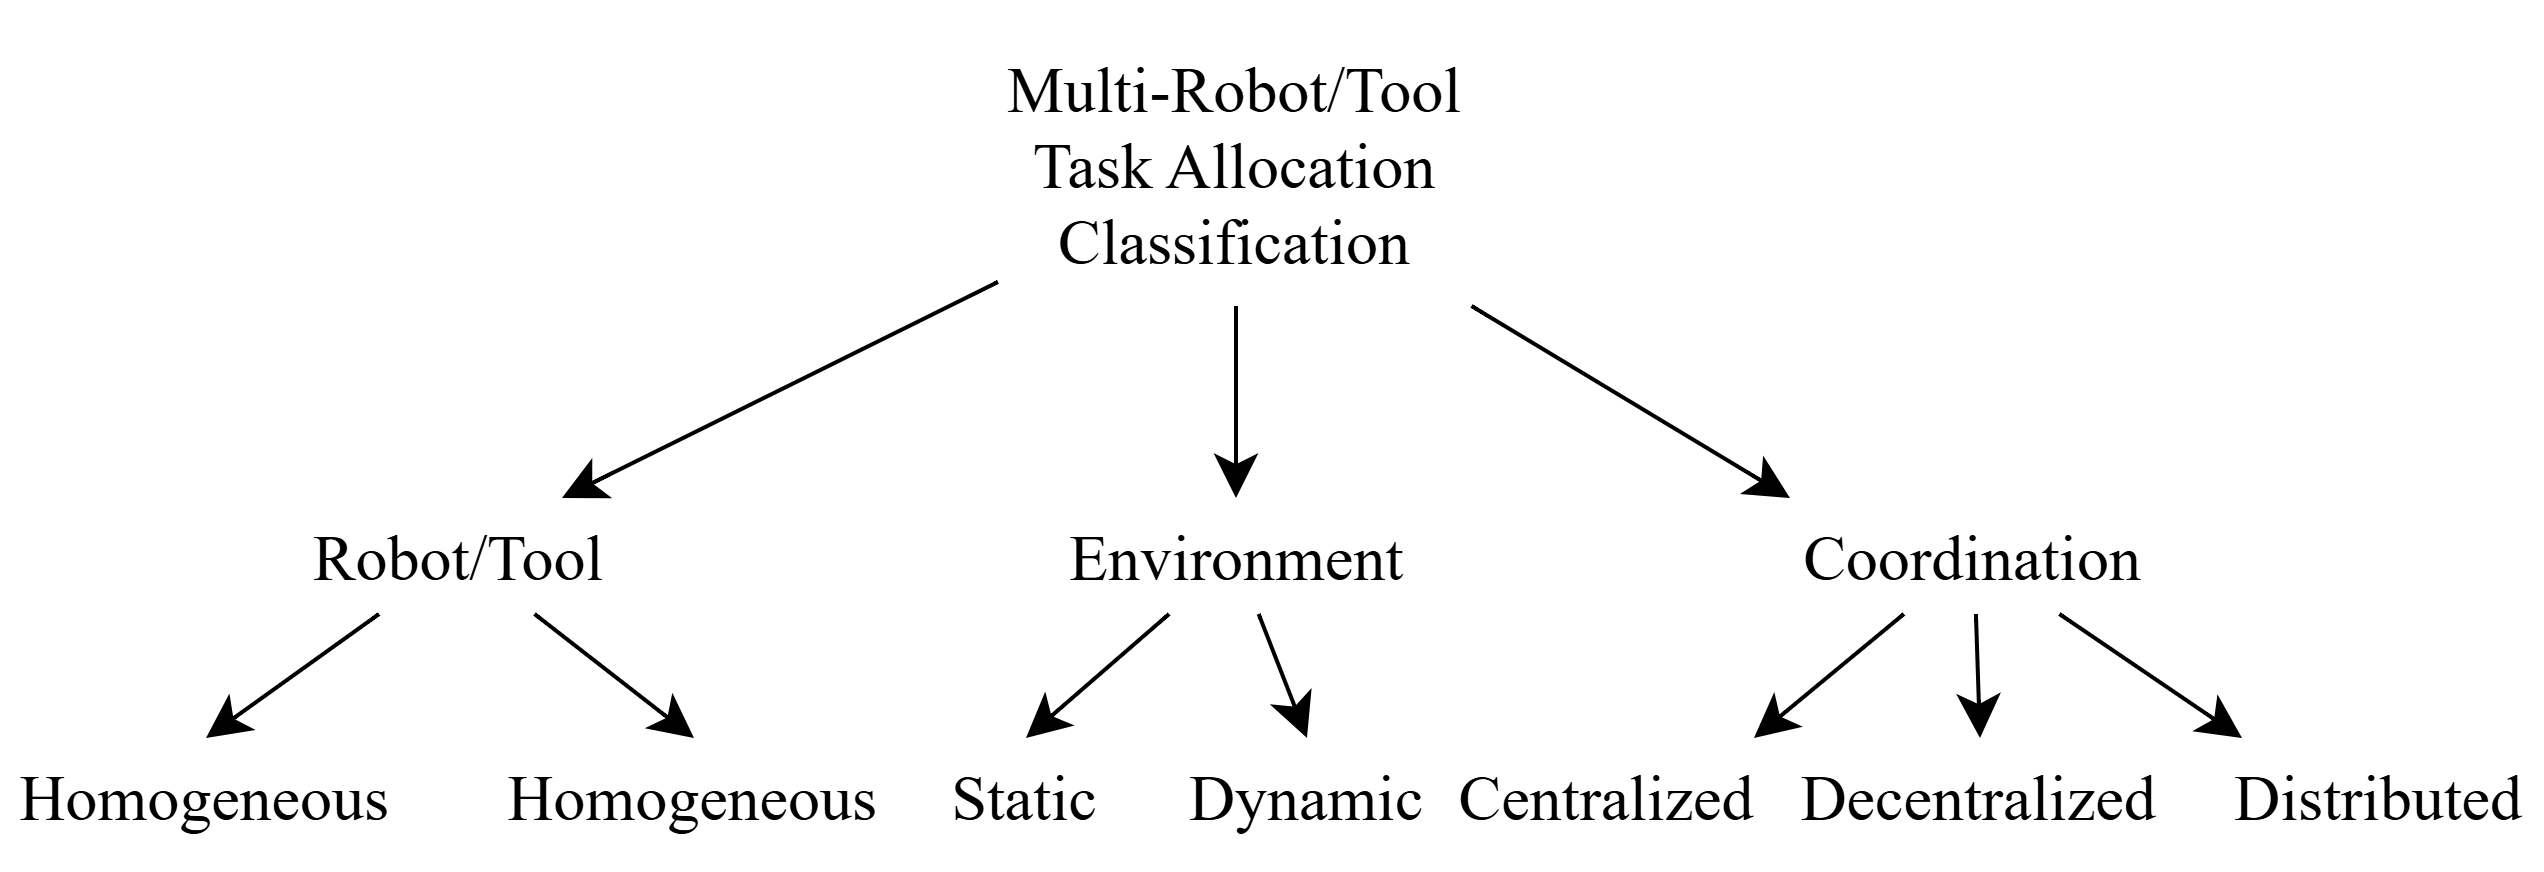
\includegraphics[width=0.9\linewidth]{gfx/ch01/task-allocation-classification.png}
    \caption{Task Allocation classification.}
    \label{fig:task-allocation-classification}
\end{figure}

An example of homogeneous tools in this context is a robot equipped with multiple tools of the same type, such as drills. In contrast, heterogeneous tools refer to robots equipped with different types of tools, such as drilling, seeding, and sensing equipment.

The multi-tool \ac{TA} can take place in either a dynamic or static environment. In an environment that is static in nature, tasks are allocated to tools in advance before they begin to execute them. This method works well in situations when the tasks are predetermined and the environment remains unchanged. In contrast, dynamic \ac{TA} involves the real-time assignment of tasks to tools as they carry out their activities. For the scope of this thesis, we will focus on homogeneous tools operating in a dynamic environment with centralized coordination, where the onboard computer will act as the master, assigning plants to each weed control mechanism.

There are several ways to accomplish multi-tool allocation, including heuristic, cluster-based, market-based, learning-based, and optimization-based techniques. Table \ref{tab:task-allocation-approaches-1} and \ref{tab:task-allocation-approaches-2} presents a comprehensive classification of \ac{TA} algorithms found in the literature \cite{Umashankar2024}.

\begin{table}[htbp]
    \myfloatalign
    \setlength{\tabcolsep}{1.5em} % Default is 0.5em
    \begin{tabularx}{\textwidth}{Xll}
        \toprule
        \tableheadline{Approach} & \tableheadline{Technique/Algorithm}                          \\
        \midrule

        \multirow{6}{*}{Cluster Based}
                                 & \acs{SVCA}\label{acro:SVCA}              \cite{Martin2023}   \\
                                 & Group Agent Partitioning                 \cite{Junyan2021}   \\
                                 & \acs{CBDTA}\label{acro:CBDTA}            \cite{Chen2018}     \\
                                 & \acs{VDKM}\label{acro:VDKM}              \cite{Kim2020}      \\
                                 & \acs{CBBA}\label{acro:CBBA}              \cite{Smith2014}    \\
                                 & K-Means Clustering                       \cite{Lu2018}       \\
        \midrule

        \multirow{7}{*}{Market Based}
                                 & Auction Algorithm                        \cite{Jiamei2022}   \\
                                 & Improved Auction Algorithm               \cite{Shiguang2021} \\
                                 & \acs{SSI}\label{acro:SSI} Auction Algorithm \cite{Dong2018}  \\
                                 & Extended \acs{SSI}                       \cite{Shi2021}      \\
                                 & Multihop-Based auction Algorithm         \cite{Lee2015}      \\
                                 & \acs{CBPAEA}\label{acro:CBPAEA}          \cite{Das2015}      \\
                                 & Distributed Auction-Based Algorithm      \cite{Luo2013}      \\
        \bottomrule
    \end{tabularx}
    \caption[Task Allocation approaches (1/2)]{Comparative overview of cluster-based and market-based approaches to Task Allocation.}
    \label{tab:task-allocation-approaches-1}
\end{table}

\begin{table}[thb]
    \myfloatalign
    \setlength{\tabcolsep}{2.5em} % Default is 0.5em
    \begin{tabularx}{\textwidth}{Xll}
        \toprule
        \tableheadline{Approach} & \tableheadline{Technique/Algorithm}                                         \\
        \midrule

        \multirow{6}{*}{Learning Based}
                                 & \acs{GRU}\label{acro:GRU}, \acs{MLP}\label{acro:MLP} \cite{Liu2022}         \\
                                 & Deep Reinforcement Learning                          \cite{Elfakharany2021} \\
                                 & Heterogeneous Graph Attention Network                \cite{Wang2022}        \\
                                 & Capsule Attention-Based Mechanism                    \cite{Paul2022}        \\
                                 & \acs{EDACAM}\label{acro:EDACAM}                      \cite{Park2022}        \\
                                 & \acf{GNN}\label{acro:GNN}                            \cite{Banfi2022}       \\
        \midrule

        \multirow{9}{*}{Optimization Based}
                                 & Mixed-Integer Quadratic Program                      \cite{Notomista2022}   \\
                                 & \acs{STADAA}\label{acro:STADAA}                      \cite{Lindsay2021}     \\
                                 & \ac{PSO}\label{acro:PSO}                             \cite{Li2020}          \\
                                 & Integer Programming                                  \cite{Velhal2022}      \\
                                 & \ac{MIQP}\label{acro:MIQP}                           \cite{Siddharth2021}   \\
                                 & \acf{GA}\label{acro:GA}                              \cite{Jose2016}        \\
                                 & \ac{COQP}\label{acro:COQP}                           \cite{Gennaro2019}     \\
                                 & Heuristic Based                                      \cite{Zhao2016}        \\
                                 & Fuzzy Optimization                                   \cite{Valero2023}      \\
        \bottomrule
    \end{tabularx}
    \caption[Task Allocation approaches (2/2)]{Comparative overview of learning-based and optimization-based approaches to Task Allocation.}
    \label{tab:task-allocation-approaches-2}
\end{table}

In cluster-based approaches, the goal is to group tasks into a predefined number of clusters. Instead of assigning a single task to each tool, the clustering approach allocates entire groups of tasks to them, reducing the number of individual task assignments and computational complexity. Clustering approaches aim to minimize travel distance and maximize task coverage by grouping tasks effectively. However, the optimal clustering of tasks still needs further exploration. Although these approaches simplify \ac{TA}, they struggle to handle dynamic changes in the environment.

An optimization-based strategy aims to select the best solution from a set of available options. These solutions are constrained by specific conditions, and the optimal one is determined based on the objective function. The objective function represents the system's ultimate goal. Some of the optimization algorithms have poor robustness to uncertainties therefore this approach is more suitable for solving well-defined and static problems focusing on theoretically optimal or near-optimal solutions. Additionally, optimization-based approaches require more computational power and are less adaptable to changing environments.

Market-based approaches effectively handle highly combinatorial optimization problems. In this method, an auctioneer informs agents about available tasks and requests bids. Each agent evaluates its capacity to complete the tasks and submits a bid accordingly. The auctioneer then assigns tasks to the agent with the most favorable bid. Generally, \ac{TA} using this approach minimizes travel time. While these methods are flexible and scalable, they may not always achieve a globally optimal solution.

Recent approaches to \ac{TA} incorporate deep learning techniques such as graph neural networks and graph convolutional networks. These types of \ac{TA} methods are commonly referred as learning-based approaches. Most learning-based approaches struggle to generalize to larger-scale problem scenarios beyond those used during training. This characteristic is especially important because real-world \ac{TA} problems frequently require modeling scenarios whose costs increase with the number of tasks and robots. Table \ref{tab:approaches-comparison} gives a comparison between all the approaches, Source \cite{Umashankar2024}.

% 4) What are the technical gaps that remain? \\

\begin{table}[H]
    \centering
    \begin{tblr}{
        width = \linewidth,
        colspec = {Q[50]Q[187]Q[254]Q[248]Q[194]},
        cell{2}{2} = {Silver,t},
        cell{2}{3} = {Silver,t},
        cell{2}{4} = {Silver,t},
        cell{2}{5} = {Silver,t},
        cell{3}{2} = {t},
        cell{3}{3} = {t},
        cell{3}{4} = {t},
        cell{3}{5} = {t},
        cell{4}{2} = {Silver,t},
        cell{4}{3} = {Silver,t},
        cell{4}{4} = {Silver,t},
        cell{4}{5} = {Silver,t},
        cell{5}{2} = {t},
        cell{5}{3} = {t},
        cell{5}{4} = {t},
        cell{5}{5} = {t},
        }
        & Clustering                            & Optimization                                                & Market                                             & Learning                                \\
        \rotatebox[origin=c]{90}{Advantage}   & Simplifies TA~and reduces complexity  & Provides optimal solutions, suited for static problems & Flexible, scalable, decentralized                        & Adaptable, learns, and improves over time     \\
        \rotatebox[origin=c]{90}{Limitation}  & May not account for dynamics well     & Computationally intensive, less adaptable                   & May not be global optima, needs effective bidding & Requires training, initially sub-optimal \\
        \rotatebox[origin=c]{90}{Best case}   & Logical tasks                         & Well-defined, static problems                               & Dynamic environments with varying tasks                  & Complex and uncertain environments            \\
        \rotatebox[origin=c]{90}{Future work} & Dynamic clustering, online adaptation & Hybrid models, real-time optimization                       & Adaptive market mechanisms, incentive models             & Transfer learning, meta-learning
    \end{tblr}
    \caption{Comparison between Task Allocation approaches}
    \label{tab:approaches-comparison}
\end{table}

\section{Proposed Solution}
% 5) What are the proposed solution approaches?
As Table \ref{tab:approaches-comparison} illustrates, algorithm selection must be carefully considered based on the application's nature to achieve optimal performance. In a grass field clearing application, the environment is highly dynamic, especially since weed detections occur while the system is in motion. Therefore, market-based approaches are well-suited to ensuring the system adapts effectively to such conditions. However, this solution might not be optimal.

Optimization-based solutions, on the other hand, are known for providing optimal results, but they are typically more suited for static problems. In our case, although the environment is dynamic, this approach is still worth exploring. Since tasks are continuously added and removed from the allocation problem, the computation time at this task density may not be a significant issue, making real-time optimization feasible.

A graph search approach is also proposed, which becomes particularly interesting if the problem can be translated into a graph representation. Using well-known algorithms such as \ac{DFS} or Dijkstra's can help find the lowest-cost solution and achieve effective resource allocation, reducing both idle time and overall mission duration.

Lastly, clustering and learning-based approaches will be discarded. Clustering due to the challenges of dynamic clustering and the need for online adaptation. Although it offers the advantage of simplifying \ac{TA}, its benefits diminish in low to medium density scenarios. Learning-based approaches are excluded because of the required training phase and the difficulty of generalizing across environments with varying task densities.
\cleardoublepage
%*****************************************
\chapter{Simulation}\label{ch:simulation}
%*****************************************
\section{The Robot}\label{sec:nuga}
Nuga is Paltech's solution for speeding up the weed removal process. Nuga is a mobile platform equipped with two drilling mechanisms, also called \ac{IT}, one main camera at the front for plant detection, two internal cameras for fine adjustment during tools' placement, an IMU, and two GNSS antennas for GPS localization. Each \ac{IT} is mounted on a structure with three \ac{DOF} using prismatic joints, allowing movement in X, Y, and Z directions.

\begin{figure}[bth]
    \centering
    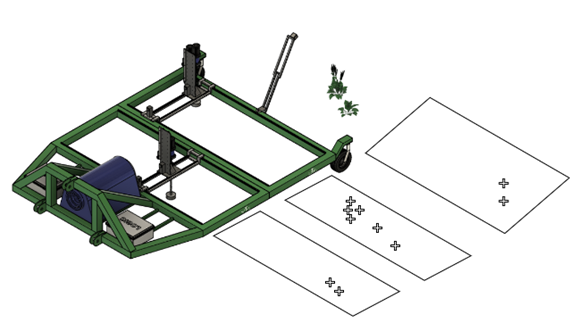
\includegraphics[width=0.7\linewidth]{gfx/ch02/nuga_cad.png}
    \caption{Nuga Platform}
    \label{fig:nuga-cad}
\end{figure}


% See classicthesis-config.tex for changing the prefixes of the refs
% Testing for autoref: \autoref{ch:intro}, \autoref{ch:examples}, and \autoref{sec:new}

%Testing for ``clever'' references: \cref{ch:intro} and \cref{ch:examples}
% Ugly work-around
% Part~\textsc{\ref{pt:showcase}}


\section{Simulation}\label{sec:simulation}
A representative simulation of reality is crucial for developing new algorithms and analyzing robot behavior before real-world implementation. Therefore, building a simulation of the project was a foundational step for this work, ensuring a controlled environment for validation and testing. Gazebo\footnote{Gazebo is a physics-based robotics simulation tool that allows testing and validation of robot models before real-world deployment. \url{https://gazebosim.org/home}} was the selected tool because it provides a physics engine, supports sensor and actuator modeling, and integrates well with ROS\footnote{ROS (Robot Operating System) is an open-source framework that provides tools, libraries, and conventions for developing, managing, and simulating robotic applications. \url{https://www.ros.org/}}, making it ideal for testing robotic systems.

The simulation consists of six key components: URDF files define the robot's structure and properties, SDF files describe the virtual environment, and Gazebo plugins provide additional functionality, such as simulating custom sensors, actuators, or control interfaces. Additionally, core system operations include joint control for managing the movement of the \ac{IT}, localization for tracking the robot’s position, and weed detection, which relies on an AI model for Rumex recognition. \autoref{fig:building-sim} illustrates these components as building blocks for the simulation.

\begin{figure}
    \centering
    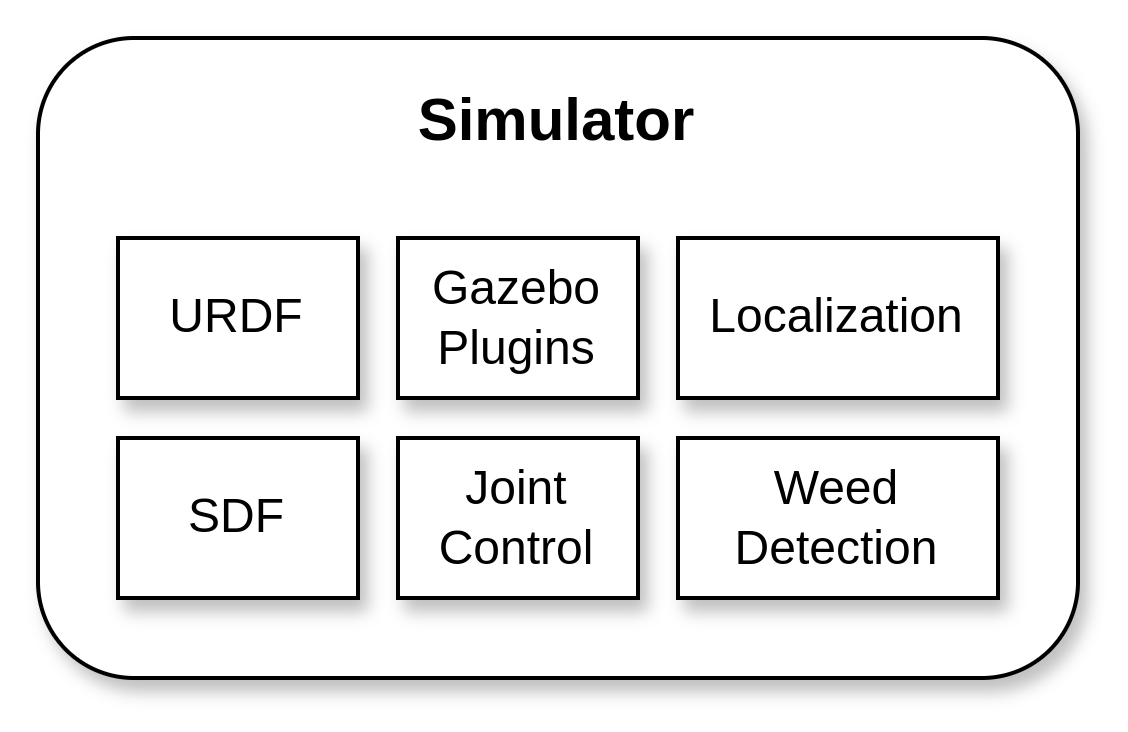
\includegraphics[width=0.5\linewidth]{gfx/ch02/simulator.png}
    \caption{Simulator Components}
    \label{fig:building-sim}
\end{figure}

\subsection{URDF}
\ac{URDF} is an XML file used to describe multibody systems for robot simulation. It defines the visual, collision, and inertial properties of rigid body objects, as well as their connections (\emph{joints}). This establishes a spatial relationship between frames, which ROS and Gazebo can later interpret for control and visualization. This file also allows modeling different types of sensors and incorporating Gazebo plugins to link it with ROS control actions. We exploit these capabilities to define camera intrinsics, IMU behavior, GPS properties, and control the \ac{IT} using \texttt{ros2\_control}\footnote{\texttt{ros2\_control} is a ROS 2 framework that provides a standardized interface for managing hardware, enabling modular and reusable control systems for robots. \url{https://control.ros.org/rolling/doc/getting_started/getting_started.html}}.

\autoref{fig:urdf-structure} displays the structure of the URDF files, being nuga the highest level entity that joins the robot description, gazebo sensor modeling and plugins, as well as \texttt{ros2\_control} configuration. Nuga description defines the robot's physical structure, including its links (e.g., chassis, wheels, camera support), joints (fixed, continuous, prismatic connections), sensors (cameras, IMU, GPS), and inertial properties. It organizes these components into a kinematic tree (e.g., base\_link -> chassis\_link -> wheels/sensors) using macros for modularity, and resulting in the model displayed in \autoref{fig:nuga-urdf}.

\begin{figure}[hbt]
    \myfloatalign
    \subfloat[URDF files structure.]
    {\label{fig:urdf-structure}
        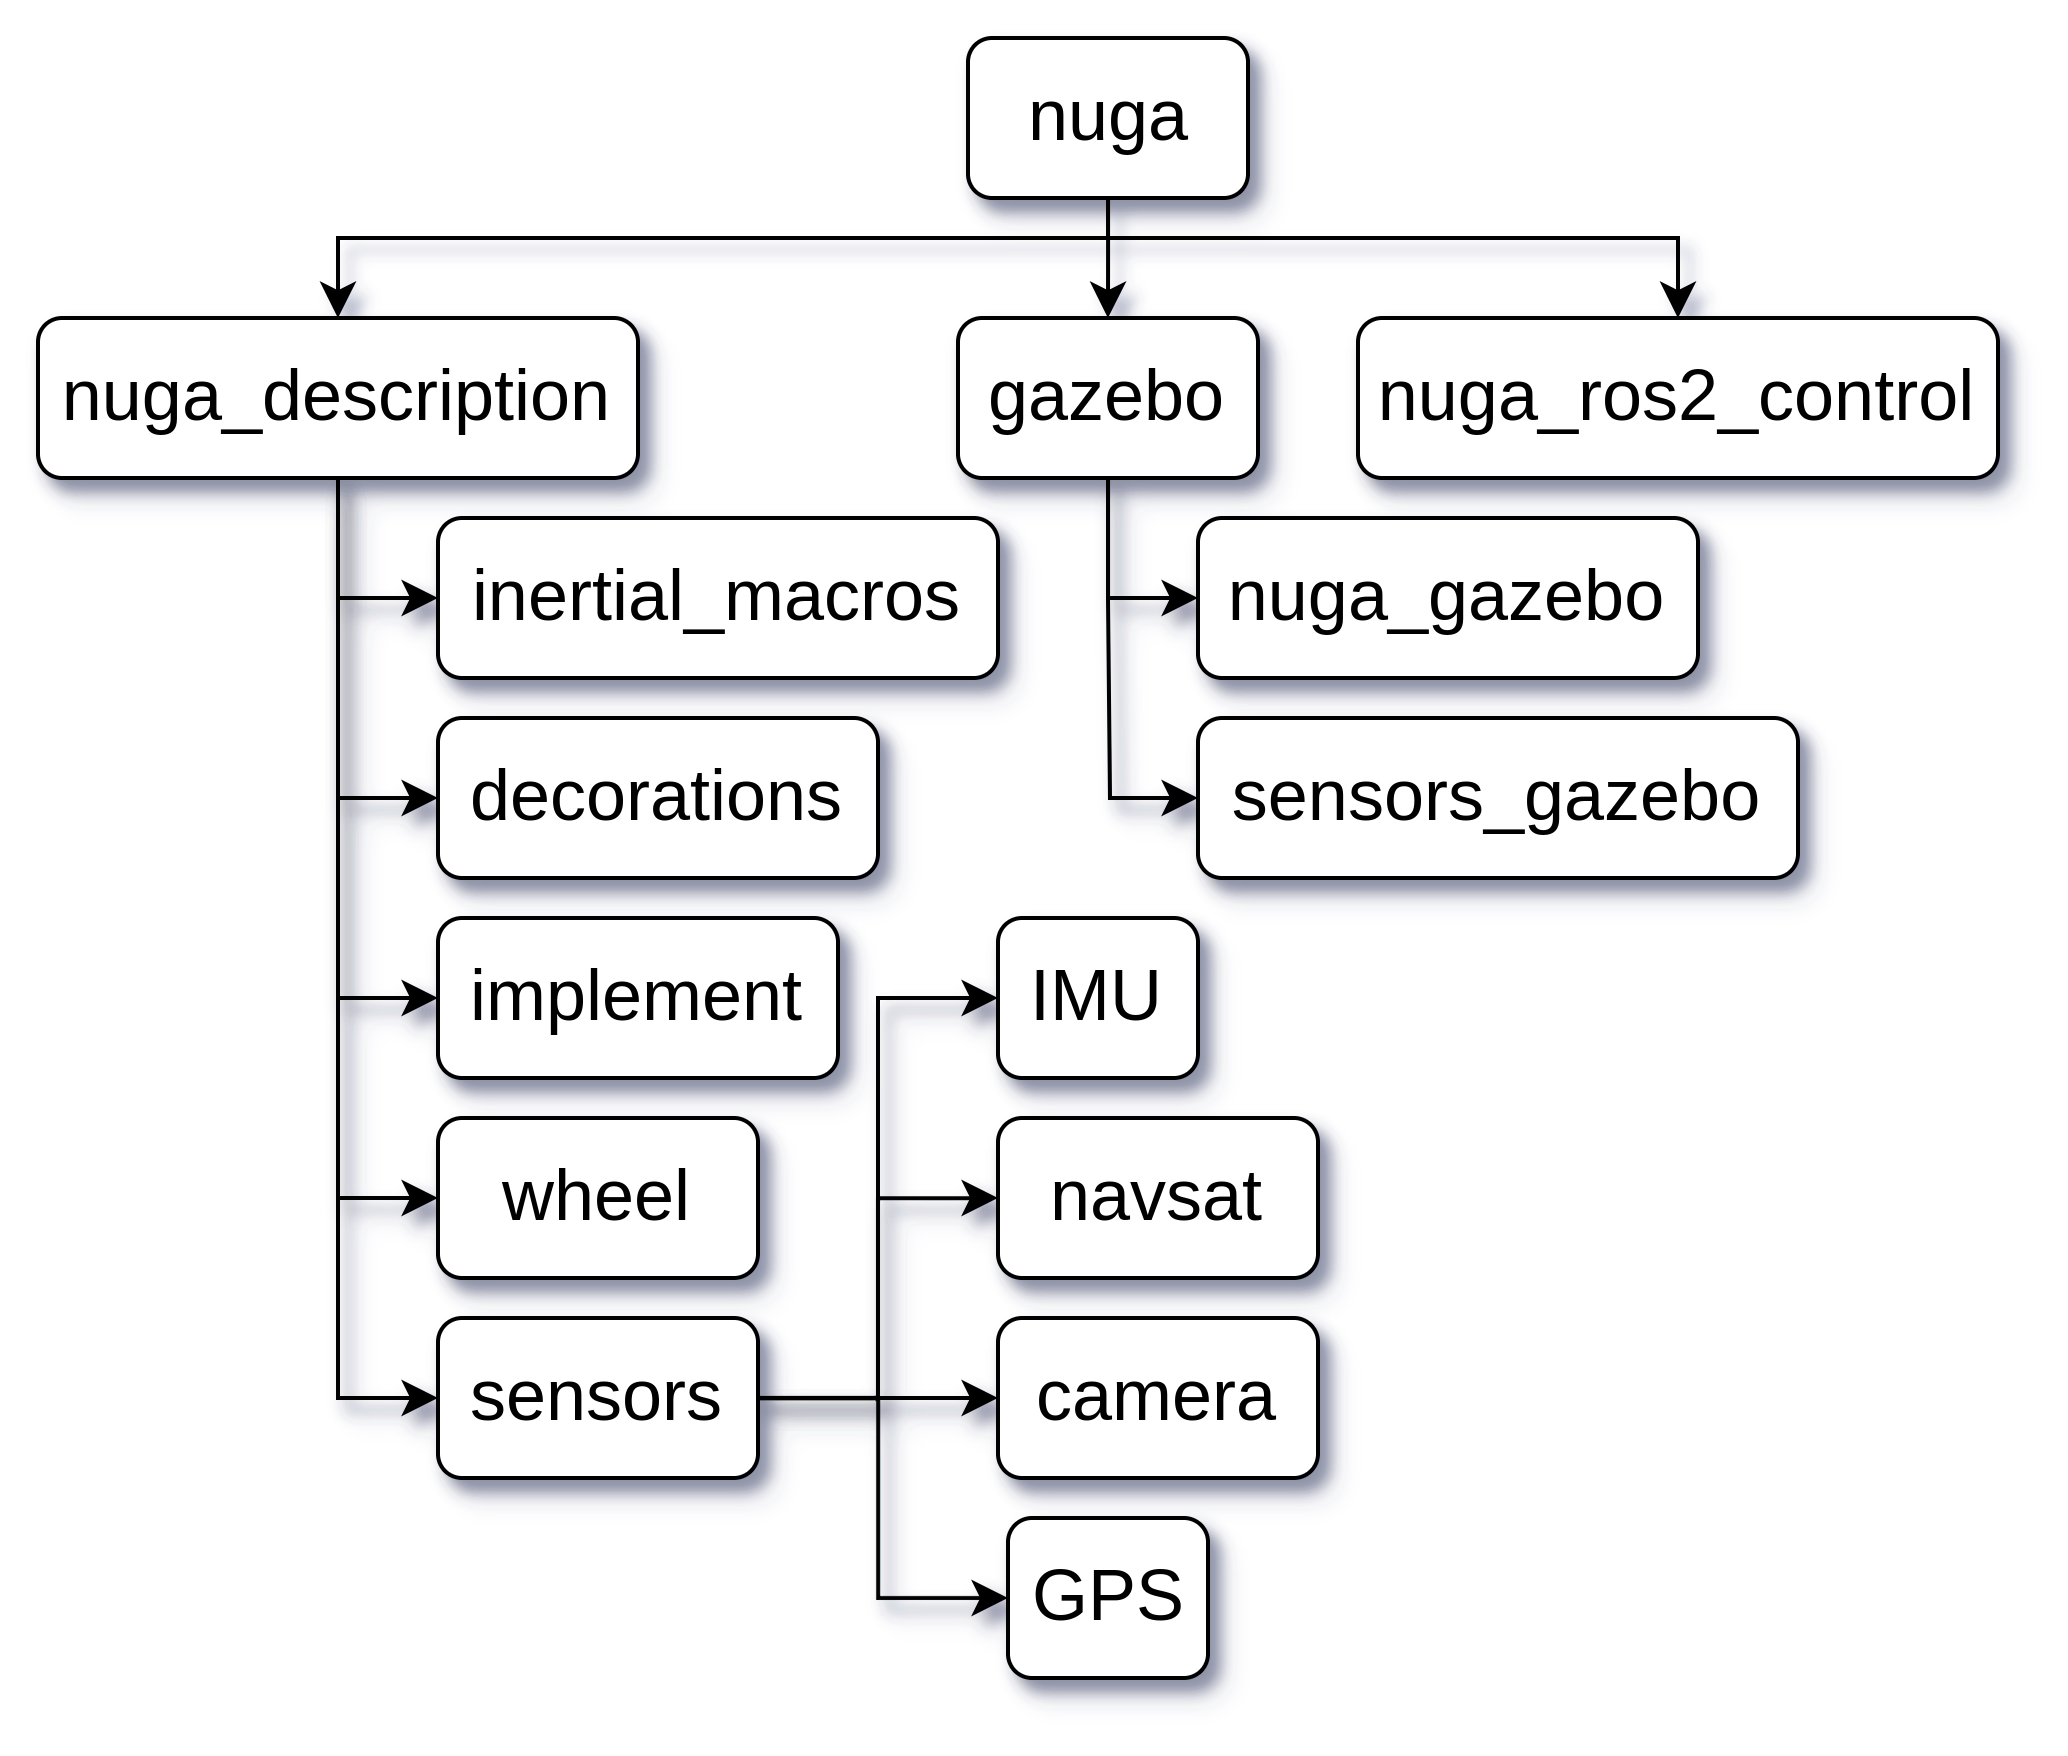
\includegraphics[width=.45\linewidth]{gfx/ch02/urdf.png}} \quad
    \subfloat[RViz visualization of Nuga description.]
    {\label{fig:nuga-urdf}%
        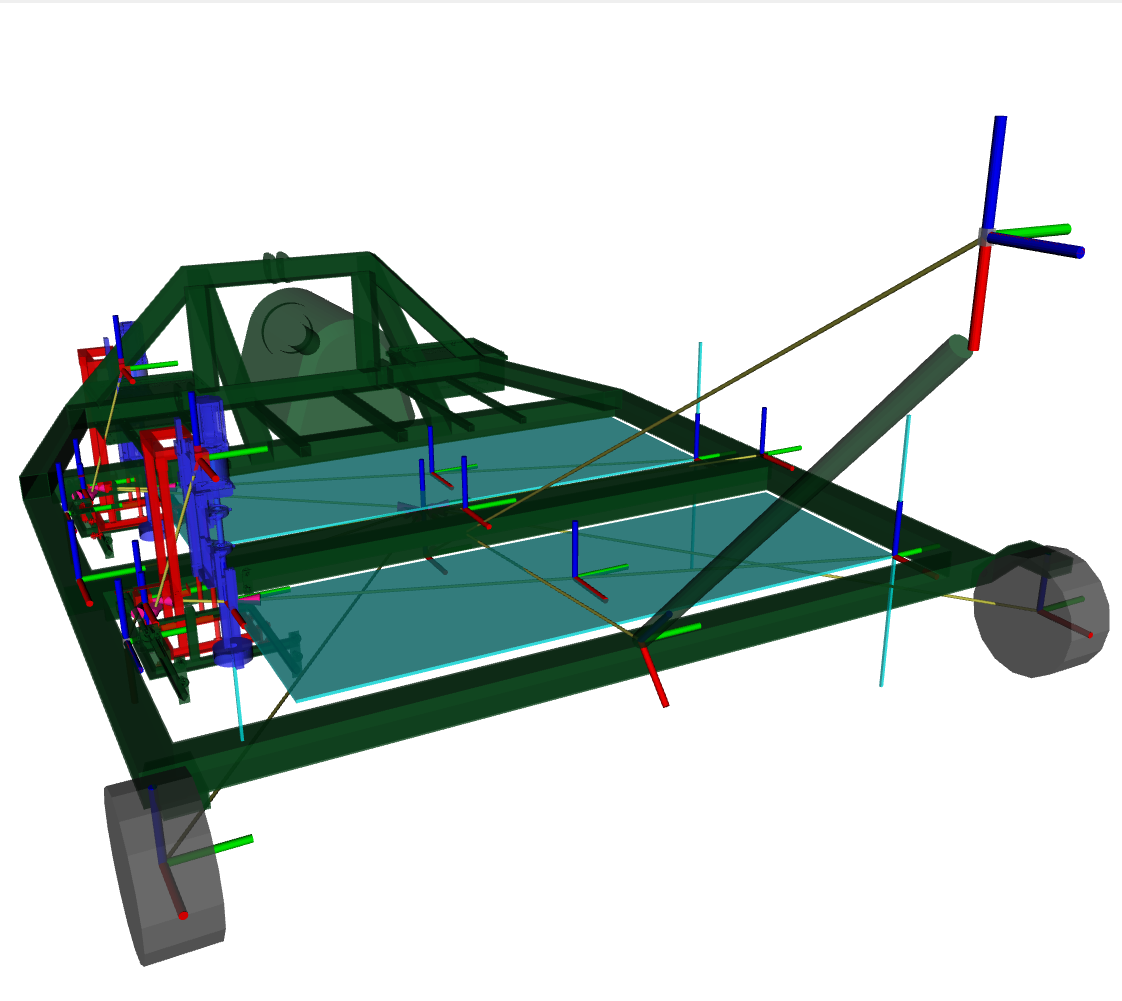
\includegraphics[width=.45\linewidth]{gfx/ch02/nuga_urdf.png}} \\
    \caption[Robot definition using URDF]{Robot definition using URDF}
\end{figure}

\subsection{SDF}
\ac{SDF} also written in XML, describes the properties of the virtual world. Gazebo uses this file to define the terrain, obstacles, lighting conditions, physics parameters, and other environmental elements that affect the robot’s interaction with the simulation. Having repeatability in a simulated world is important for debuging and testing purposes, for this reason a Python script was used to generate easy to configure worlds from a YAML configuration file. An example of the config file is shown in \autoref{lst:world-yaml}. For reproducibility, a seed value is configured in the simulation settings, the weed infestation pattern is defined within quadrants of specified dimensions (\texttt{quadrant\_size}) and each quadrant is individually configured with:

\begin{itemize}
    \item Spatial distribution:
    \begin{itemize}
        \item \textit{uniform}: Random uniform distribution
        \item \textit{clustered}: Random normal distribution with definable standard deviations ($\sigma_x, \sigma_y$)
    \end{itemize}
    \item Weed density: Weeds per square meter (weeds/m²)
    \item Direction: Propagation axis for adjacent quadrants ($\pm x,\pm y$)
    \item Workspace expansion: If \texttt{outside\_workspace} is true, the infestation area extends 10\% beyond the quadrant boundaries.
\end{itemize}

A visual result of the generated world using such configuration file is shown in \autoref{fig:world}.

\begin{figure}[h]
    \centering
    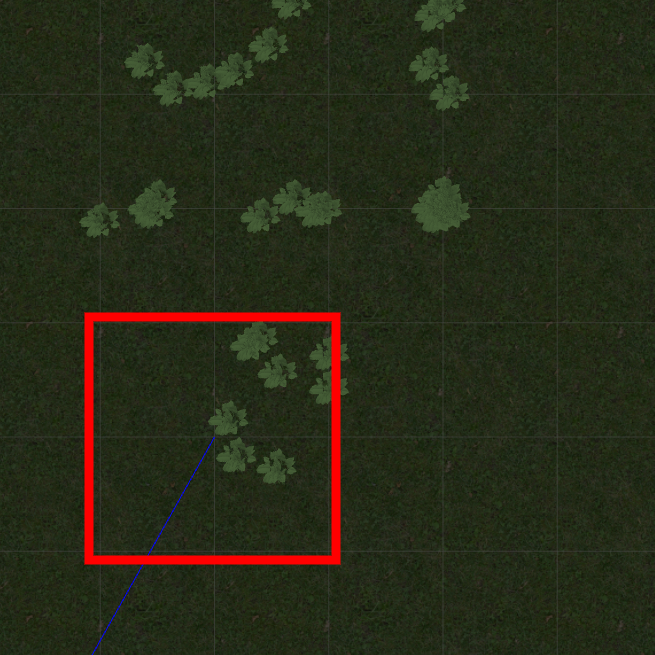
\includegraphics[width=0.4\linewidth]{gfx/ch02/world.png}
    \caption{Weed Infestation Example}
    \label{fig:world}
\end{figure}

\subsection{Gazebo Plugins}
The files \texttt{nuga\_gazebo} and \texttt{sensors\_gazebo} from \autoref{fig:urdf-structure} instantiate and configure Gazebo plugins to define sensor behavior, including optical properties for the camera, as well as update rates and noise models for the IMU and GPS. The file \texttt{nuga\_ros2\_control} on the other hand, establishes an interface between the \ac{IT} 's joints and \texttt{ros2\_control} framework, specifying the command interface (position), controller type (forward position controller), and movement limits, enabling 3-\ac{DOF} prismatic motion for each tool. Regarding movement control of the Nuga vehicle, the \texttt{ros\_planar\_move} plugin satisfied all control requirements given the platform's kinematic constraints, eliminating the need for additional configuration.

\subsection{Joint Control}
The control of both \ac{IT} units was handled using the \texttt{ros2\_control} framework (configuration example shown in \autoref{lst:ros2_control-yaml}), as previously described. This framework provides a seamless transition between simulation and real hardware control. In this context, the \texttt{forward\_command\_controller} was used, which is recommended for simulation because it bypasses PID computations by directly sending commands to simulated joints. These joints already track positions perfectly, without the disturbances or error correction needed in real-world scenarios. Simulators like Gazebo inherently handle ideal position tracking, making closed-loop control redundant. However, when switching to real hardware, replacing it with a \texttt{position\_controller} is needed but straightforward thanks to the flexibility of the framework.

Nuga's workspace layout and dimensions are shown in \autoref{fig:ws}. The gantry carrying the \ac{IT} operates within a zone of $2.09$ m in the $Y$ direction, $0.72$ m in $X$, and $0.26$ m in $Z$. An extraction cycle begins with the gantry moving in $X$ and $Y$ to position the tool above the plant, followed by a downward movement in $Z$ to lower the drill and perform the extraction. The gantry has a maximum speed of $1\frac{m}{s}$ in the $XY$ plane, and each extraction can take up to $45$ seconds per plant. 

\begin{figure}[t]
    \myfloatalign
    \subfloat[$X,Y$ Workspace]
    {\label{fig:xy-ws}
        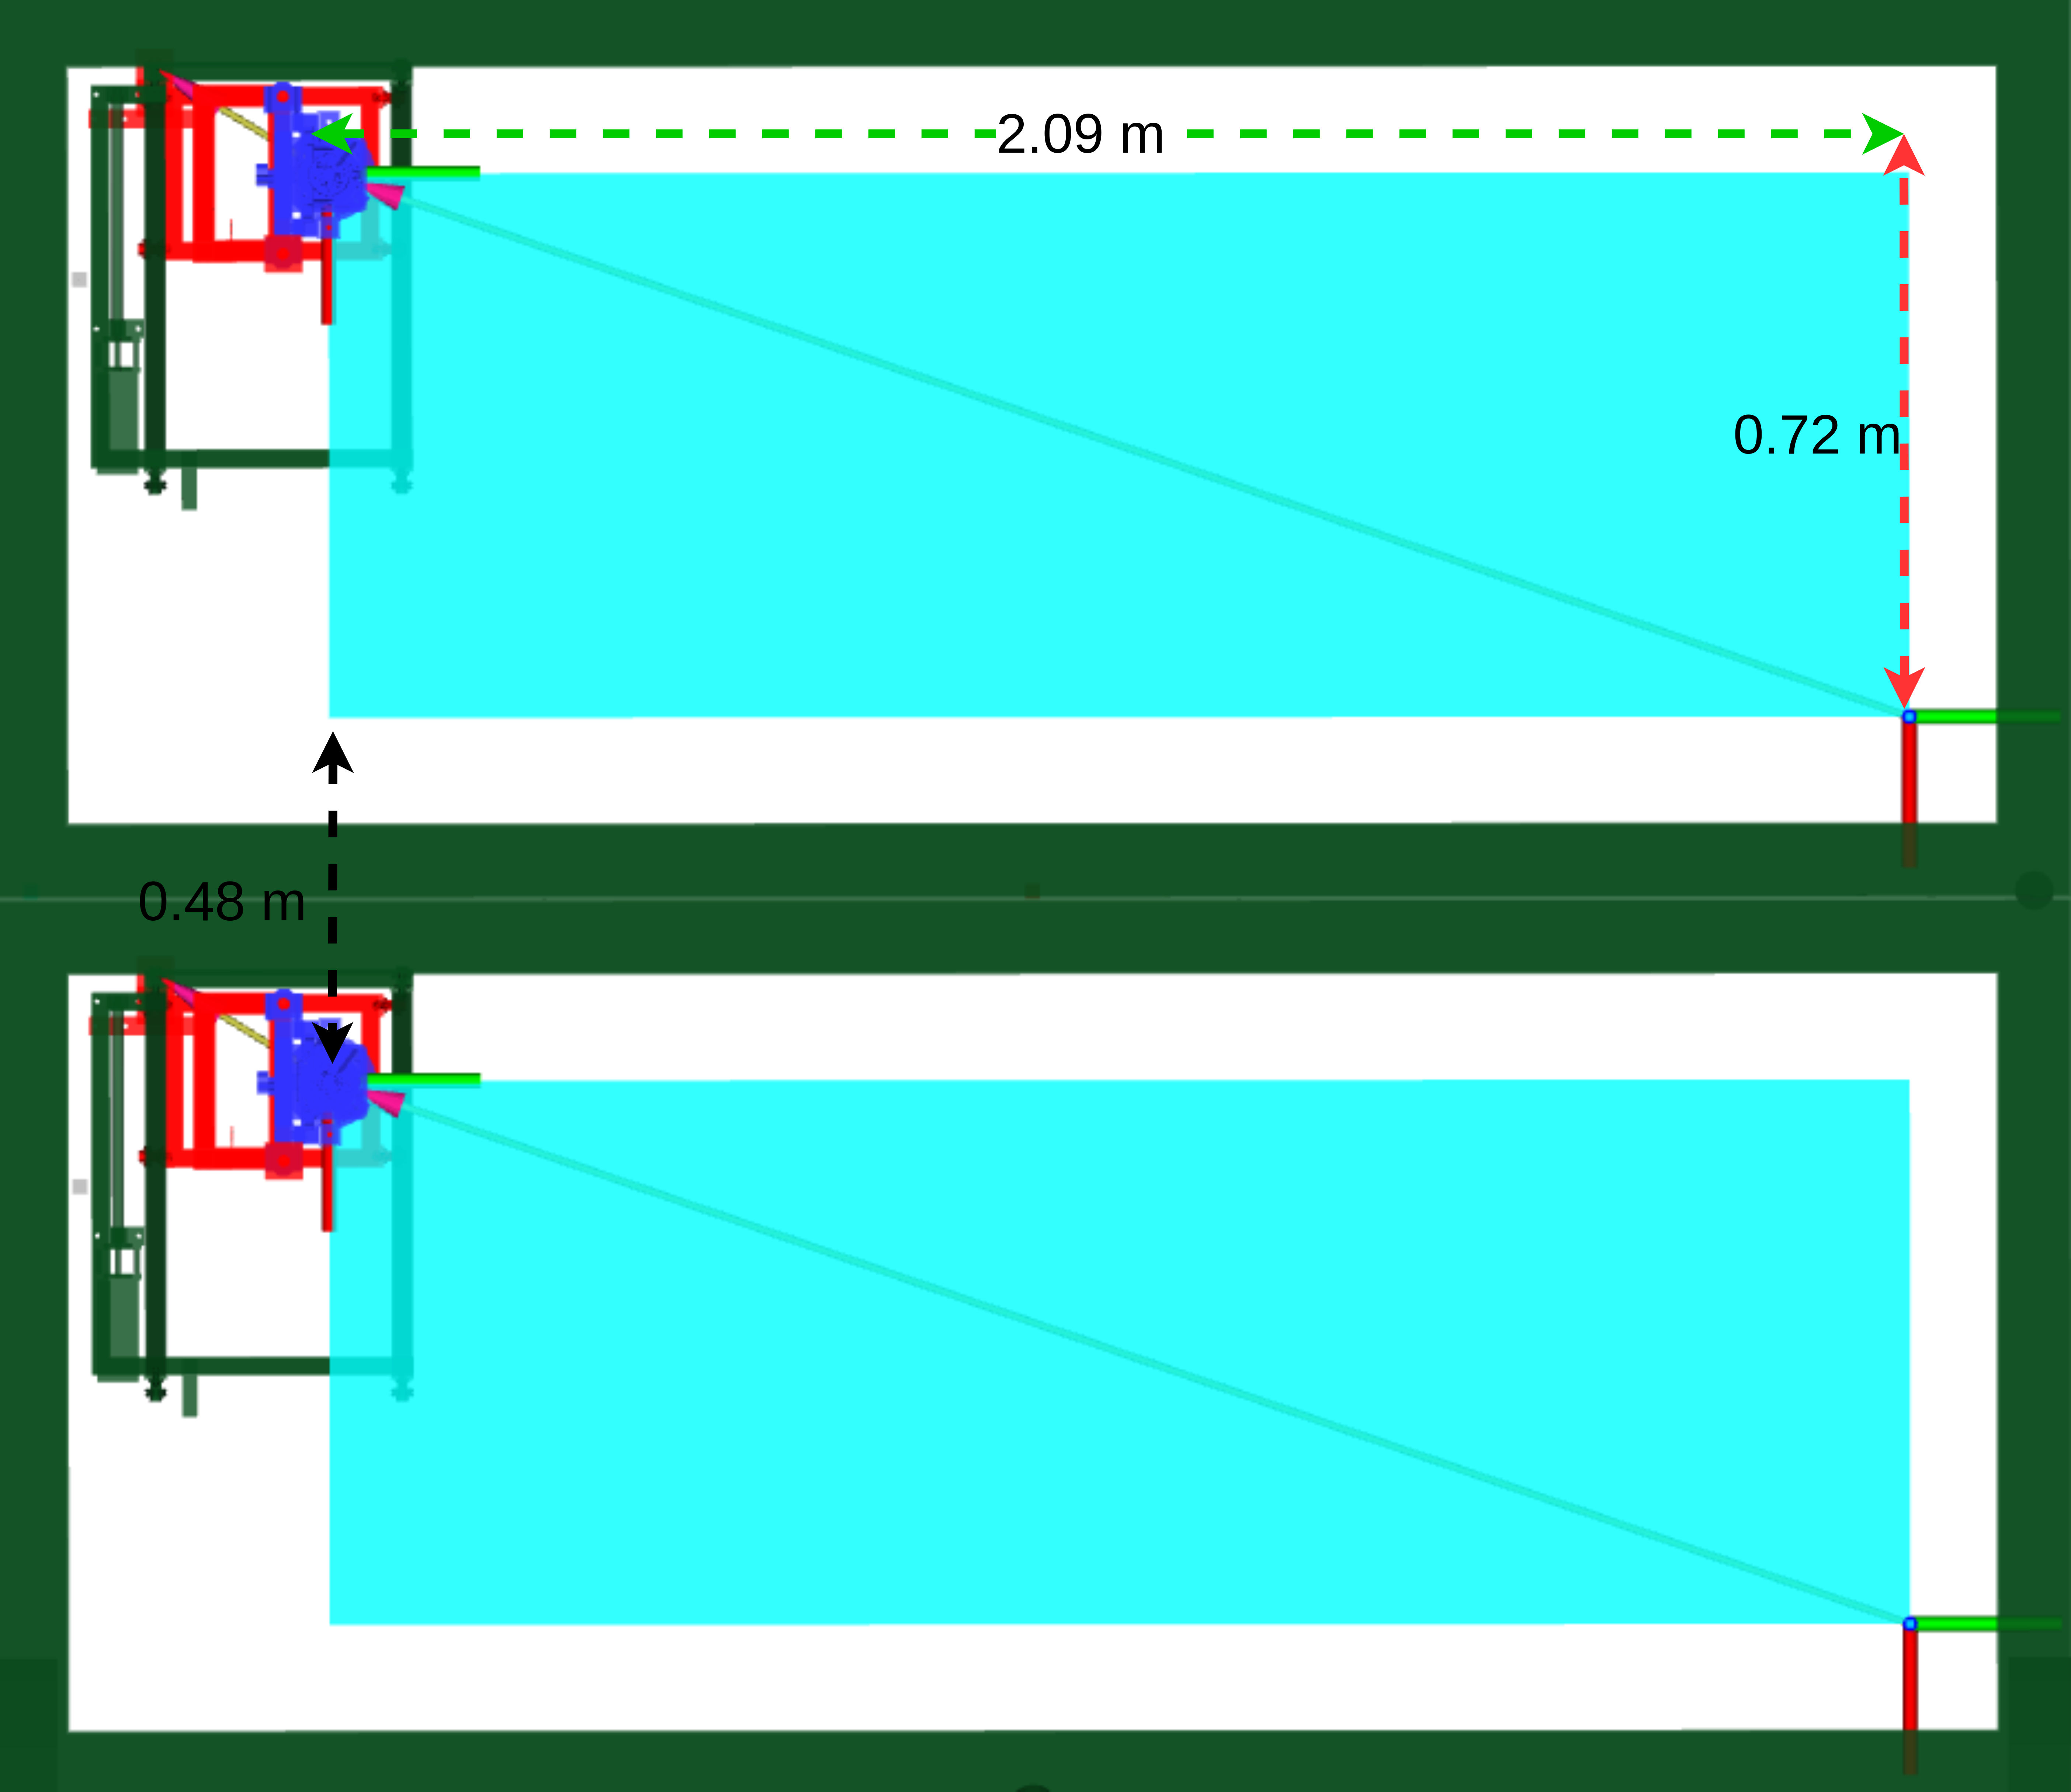
\includegraphics[width=.45\linewidth]{gfx/ch02/xy_ws.png}} \quad
    \subfloat[$Z$ Workspace]
    {\label{fig:z-ws}%
        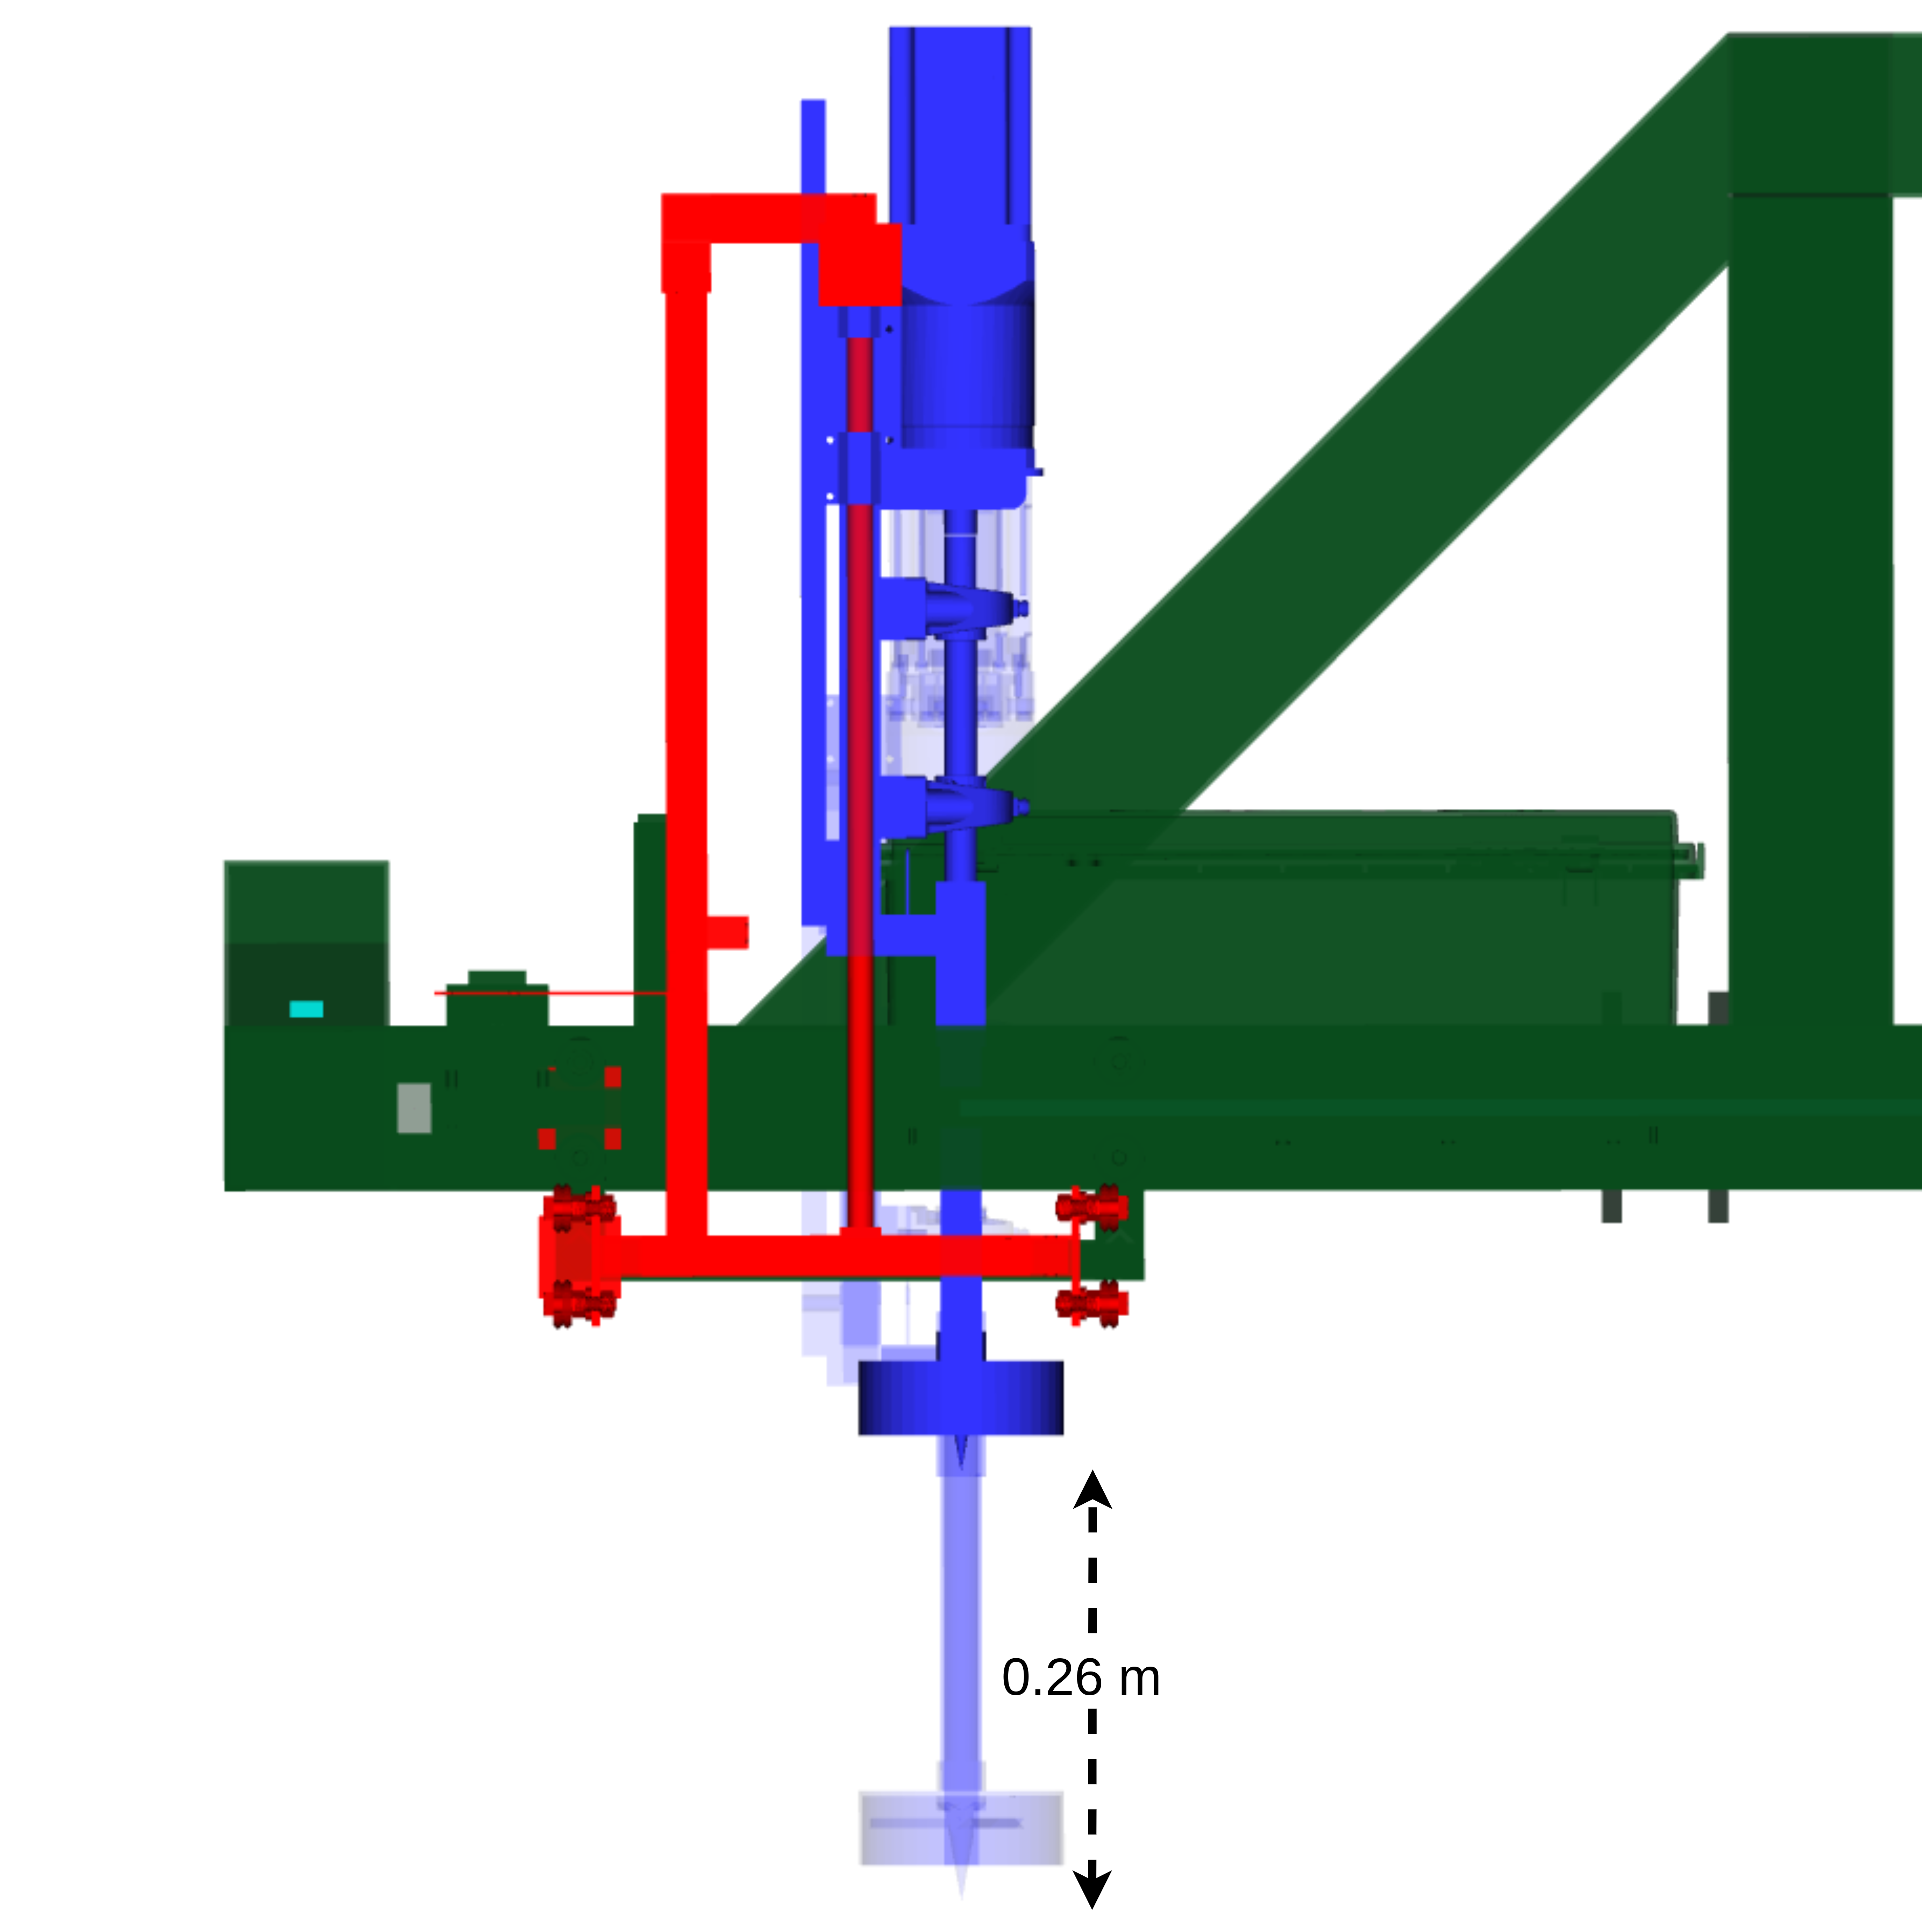
\includegraphics[width=.45\linewidth]{gfx/ch02/z_ws.png}} \\
    \caption{\ac{IT} Workspace Layout}\label{fig:ws}
\end{figure}

The \ac{IT} is controlled using ROS$2$ actions, which provide a structured way to handle asynchronous tasks with feedback and result reporting. For the $XY$ movement of the gantry, the \texttt{AxisPosition} action is used, allowing the specification of target coordinates ($x$, $y$) and speed, while providing feedback on the current position and confirming whether the target was reached. The \texttt{Extraction} action manages the vertical movement of the tool along the $Z$ axis, reporting the depth reached, total time taken, and success status, along with real-time feedback on the current depth. Finally, the \texttt{ExtractionCycle} action coordinates the execution of multiple extractions by accepting an array of target poses and their corresponding IDs, providing feedback on the current status and reporting the results of the extraction process for each pose. These actions enable precise and modular control of the gantry system, ensuring efficient and reliable operation. A diagram summarizing this process is shown in \autoref{fig:gantry-control}.

\begin{figure}[h]
    \centering
    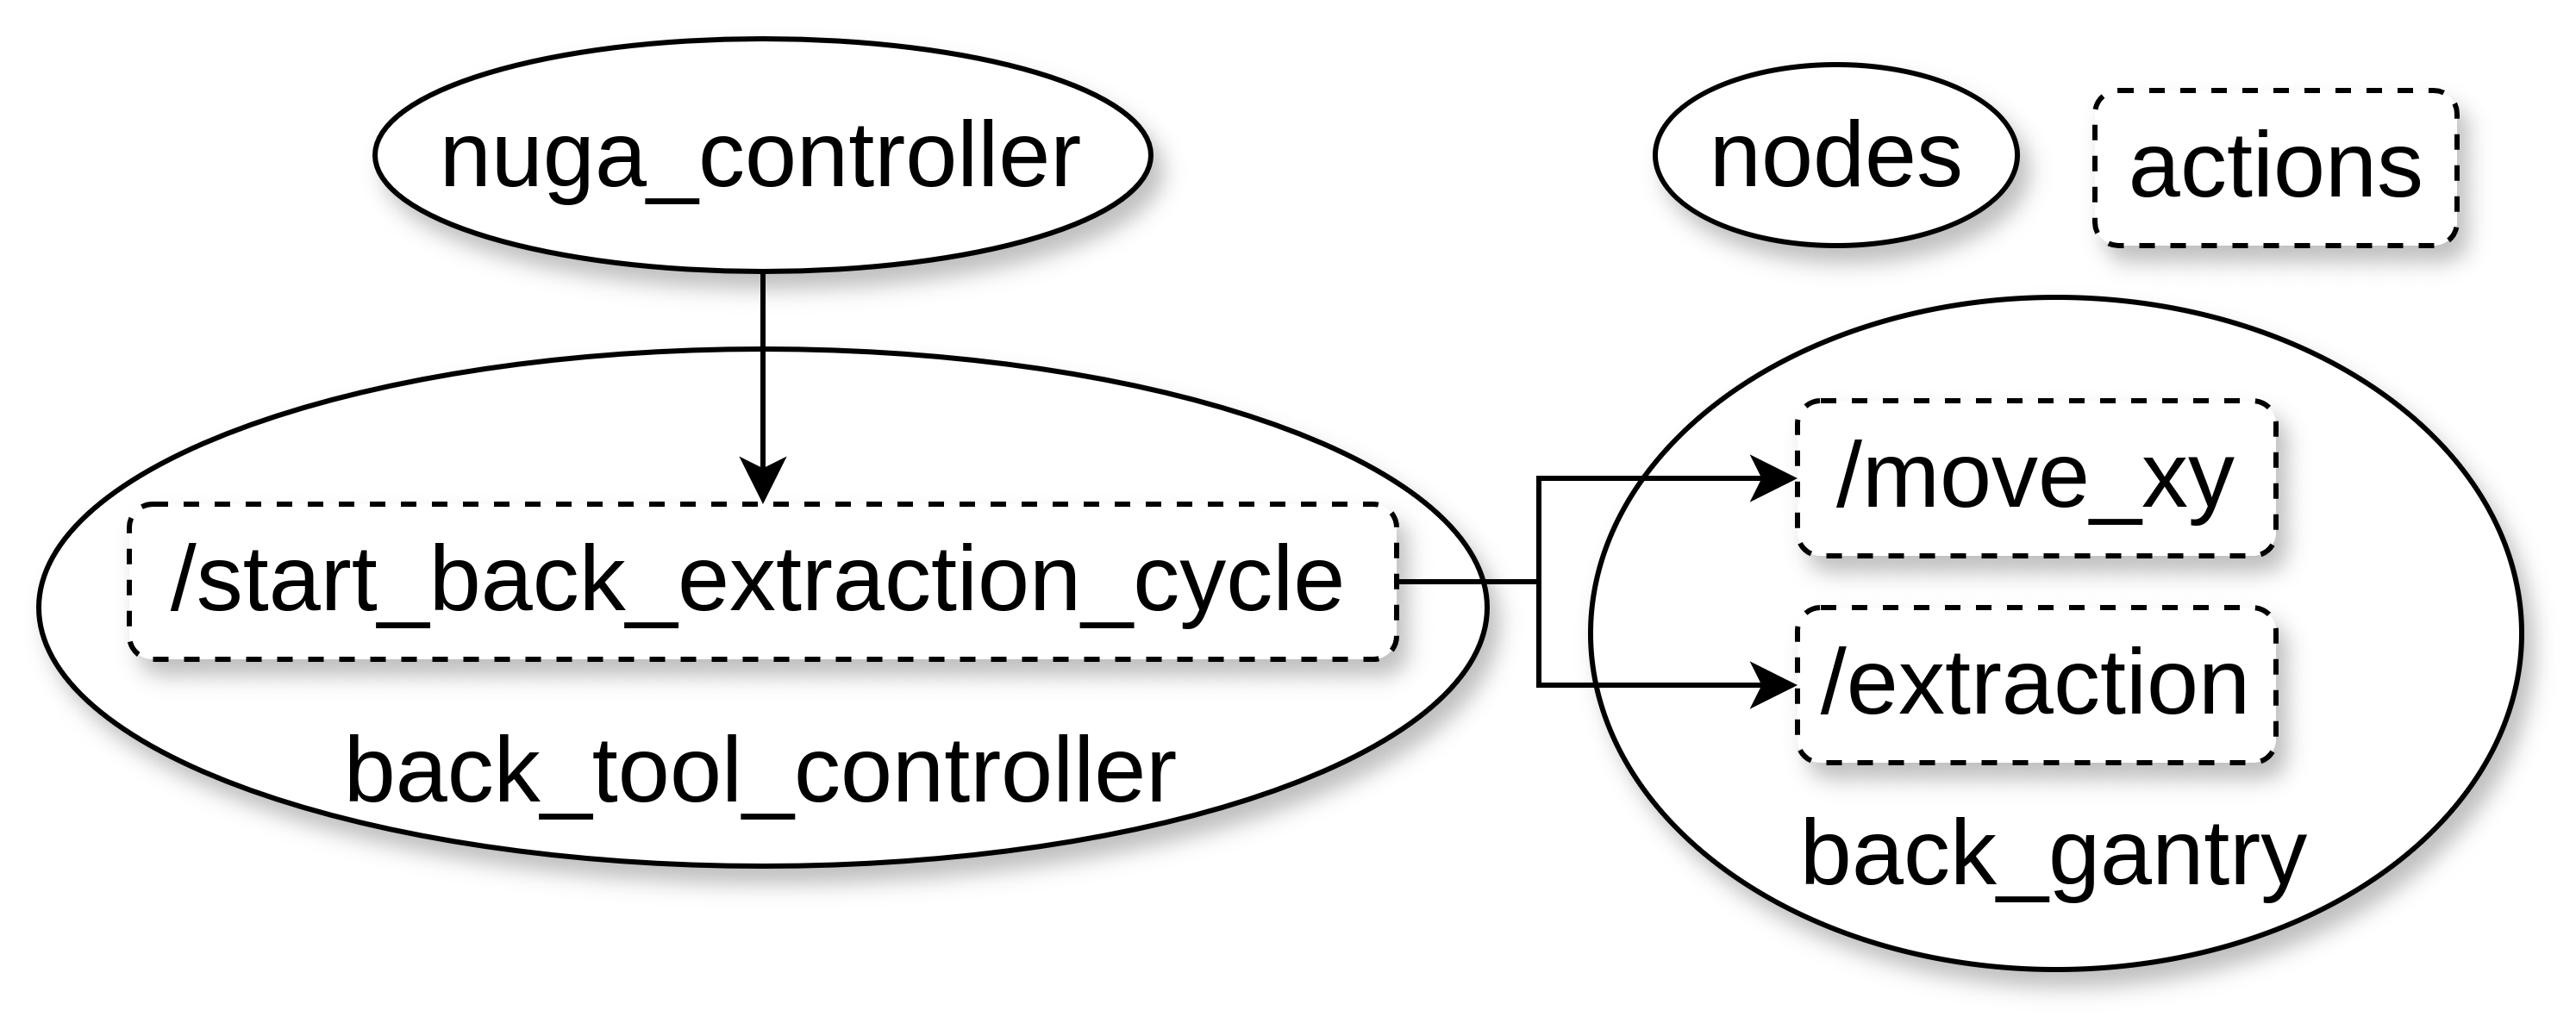
\includegraphics[width=0.7\linewidth]{gfx/ch02/gantry_control.png}
    \caption{ROS Interface for back gantry control}
    \label{fig:gantry-control}
\end{figure}


\subsection{Localization}
\lipsum[1]

\subsection{Weed Detection}
Paltech uses an in-house machine learning model for Rumex recognition, trained on a dataset of images captured under various lighting conditions. The model is integrated into the simulation using a ROS2 node that subscribes to the camera topic and publishes detection results. This node processes camera images, applies the trained model, and outputs the detected plants’ positions in camera coordinates along with confidence scores. This integration enables real-time detection of Rumex within the simulated environment, supporting planning and execution of extraction tasks. The model’s training dataset includes images such as the one shown in \autoref{fig:rumex-trainning}, and it is capable of generalizing to simulation images, as illustrated in \autoref{fig:rumex-sim}.

\begin{figure}[htb]
    \myfloatalign
    \subfloat[Trainning dataset image]
    {\label{fig:rumex-trainning}%
        \includegraphics[width=.45\linewidth]{gfx/ch02/rumex.png}} \quad
    \subfloat[Weed detection in simulation]
    {\label{fig:rumex-sim}
        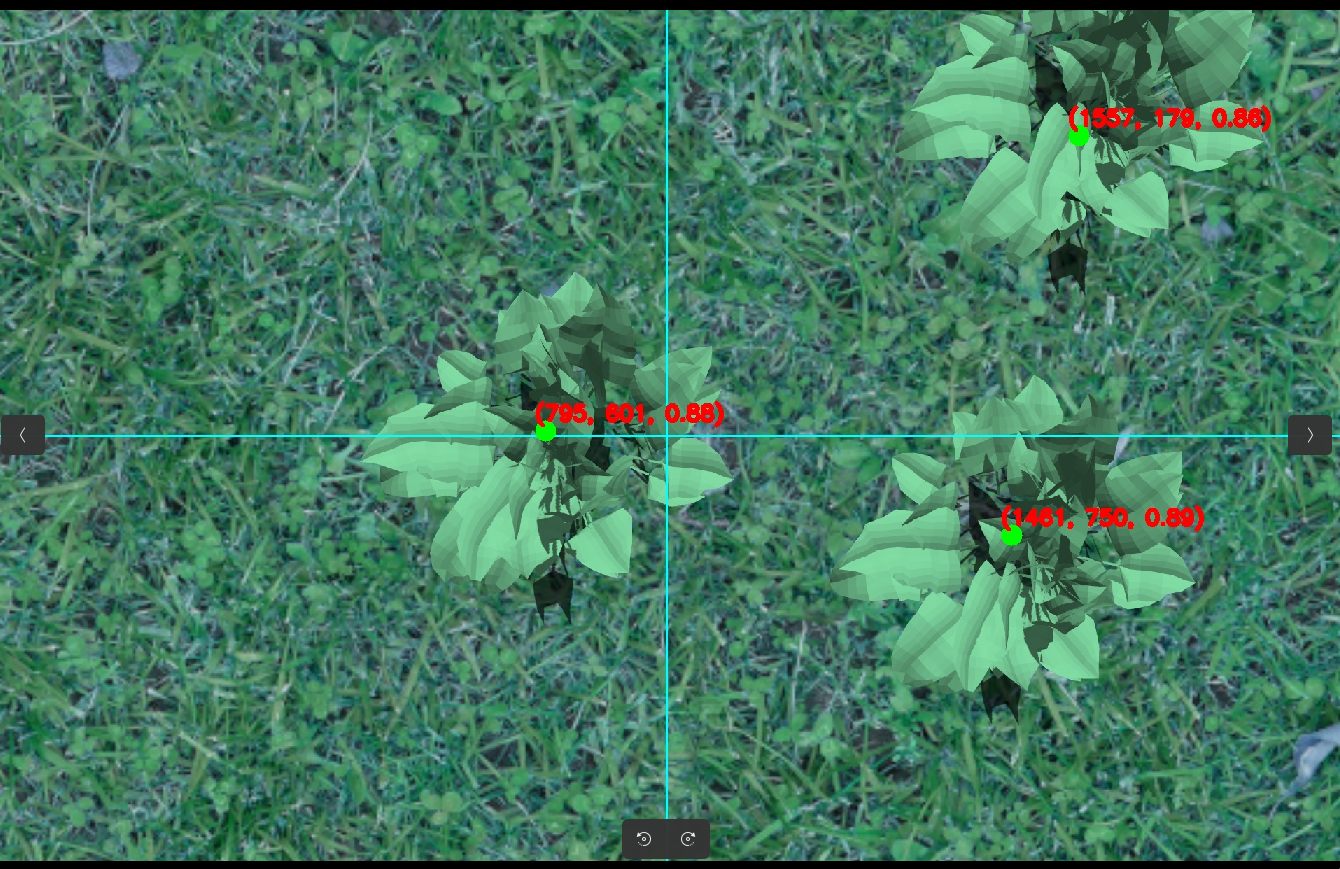
\includegraphics[width=.45\linewidth]{gfx/ch02/rumex_sim.png}} \\
    \caption{Example of trainning and detection}\label{fig:rumex-example}
\end{figure}

\subsection{Nuga Controller}
The Nuga controller is the main node responsible for orchestrating the movement of the robot, managing the \ac{IT} units, and performing task allocation based on the weed positions received from the detection node. A high-level overview of the controller's operation is shown in \autoref{fig:nuga-controller}. The timer callbacks \texttt{get\_ws\_limits()} and \texttt{get\_imp\_offsets()} are self-destructive timers used to retrieve the positions of the tool workspace limits and their offsets relative to the \texttt{base\_link}. Once this information is received, the timers are destroyed. The same applies to the callback of the \textit{/head\_camera/camera\_info} topic, which is used to obtain the camera’s central pixel position for later use.

\begin{figure}[ht]
    \centering
    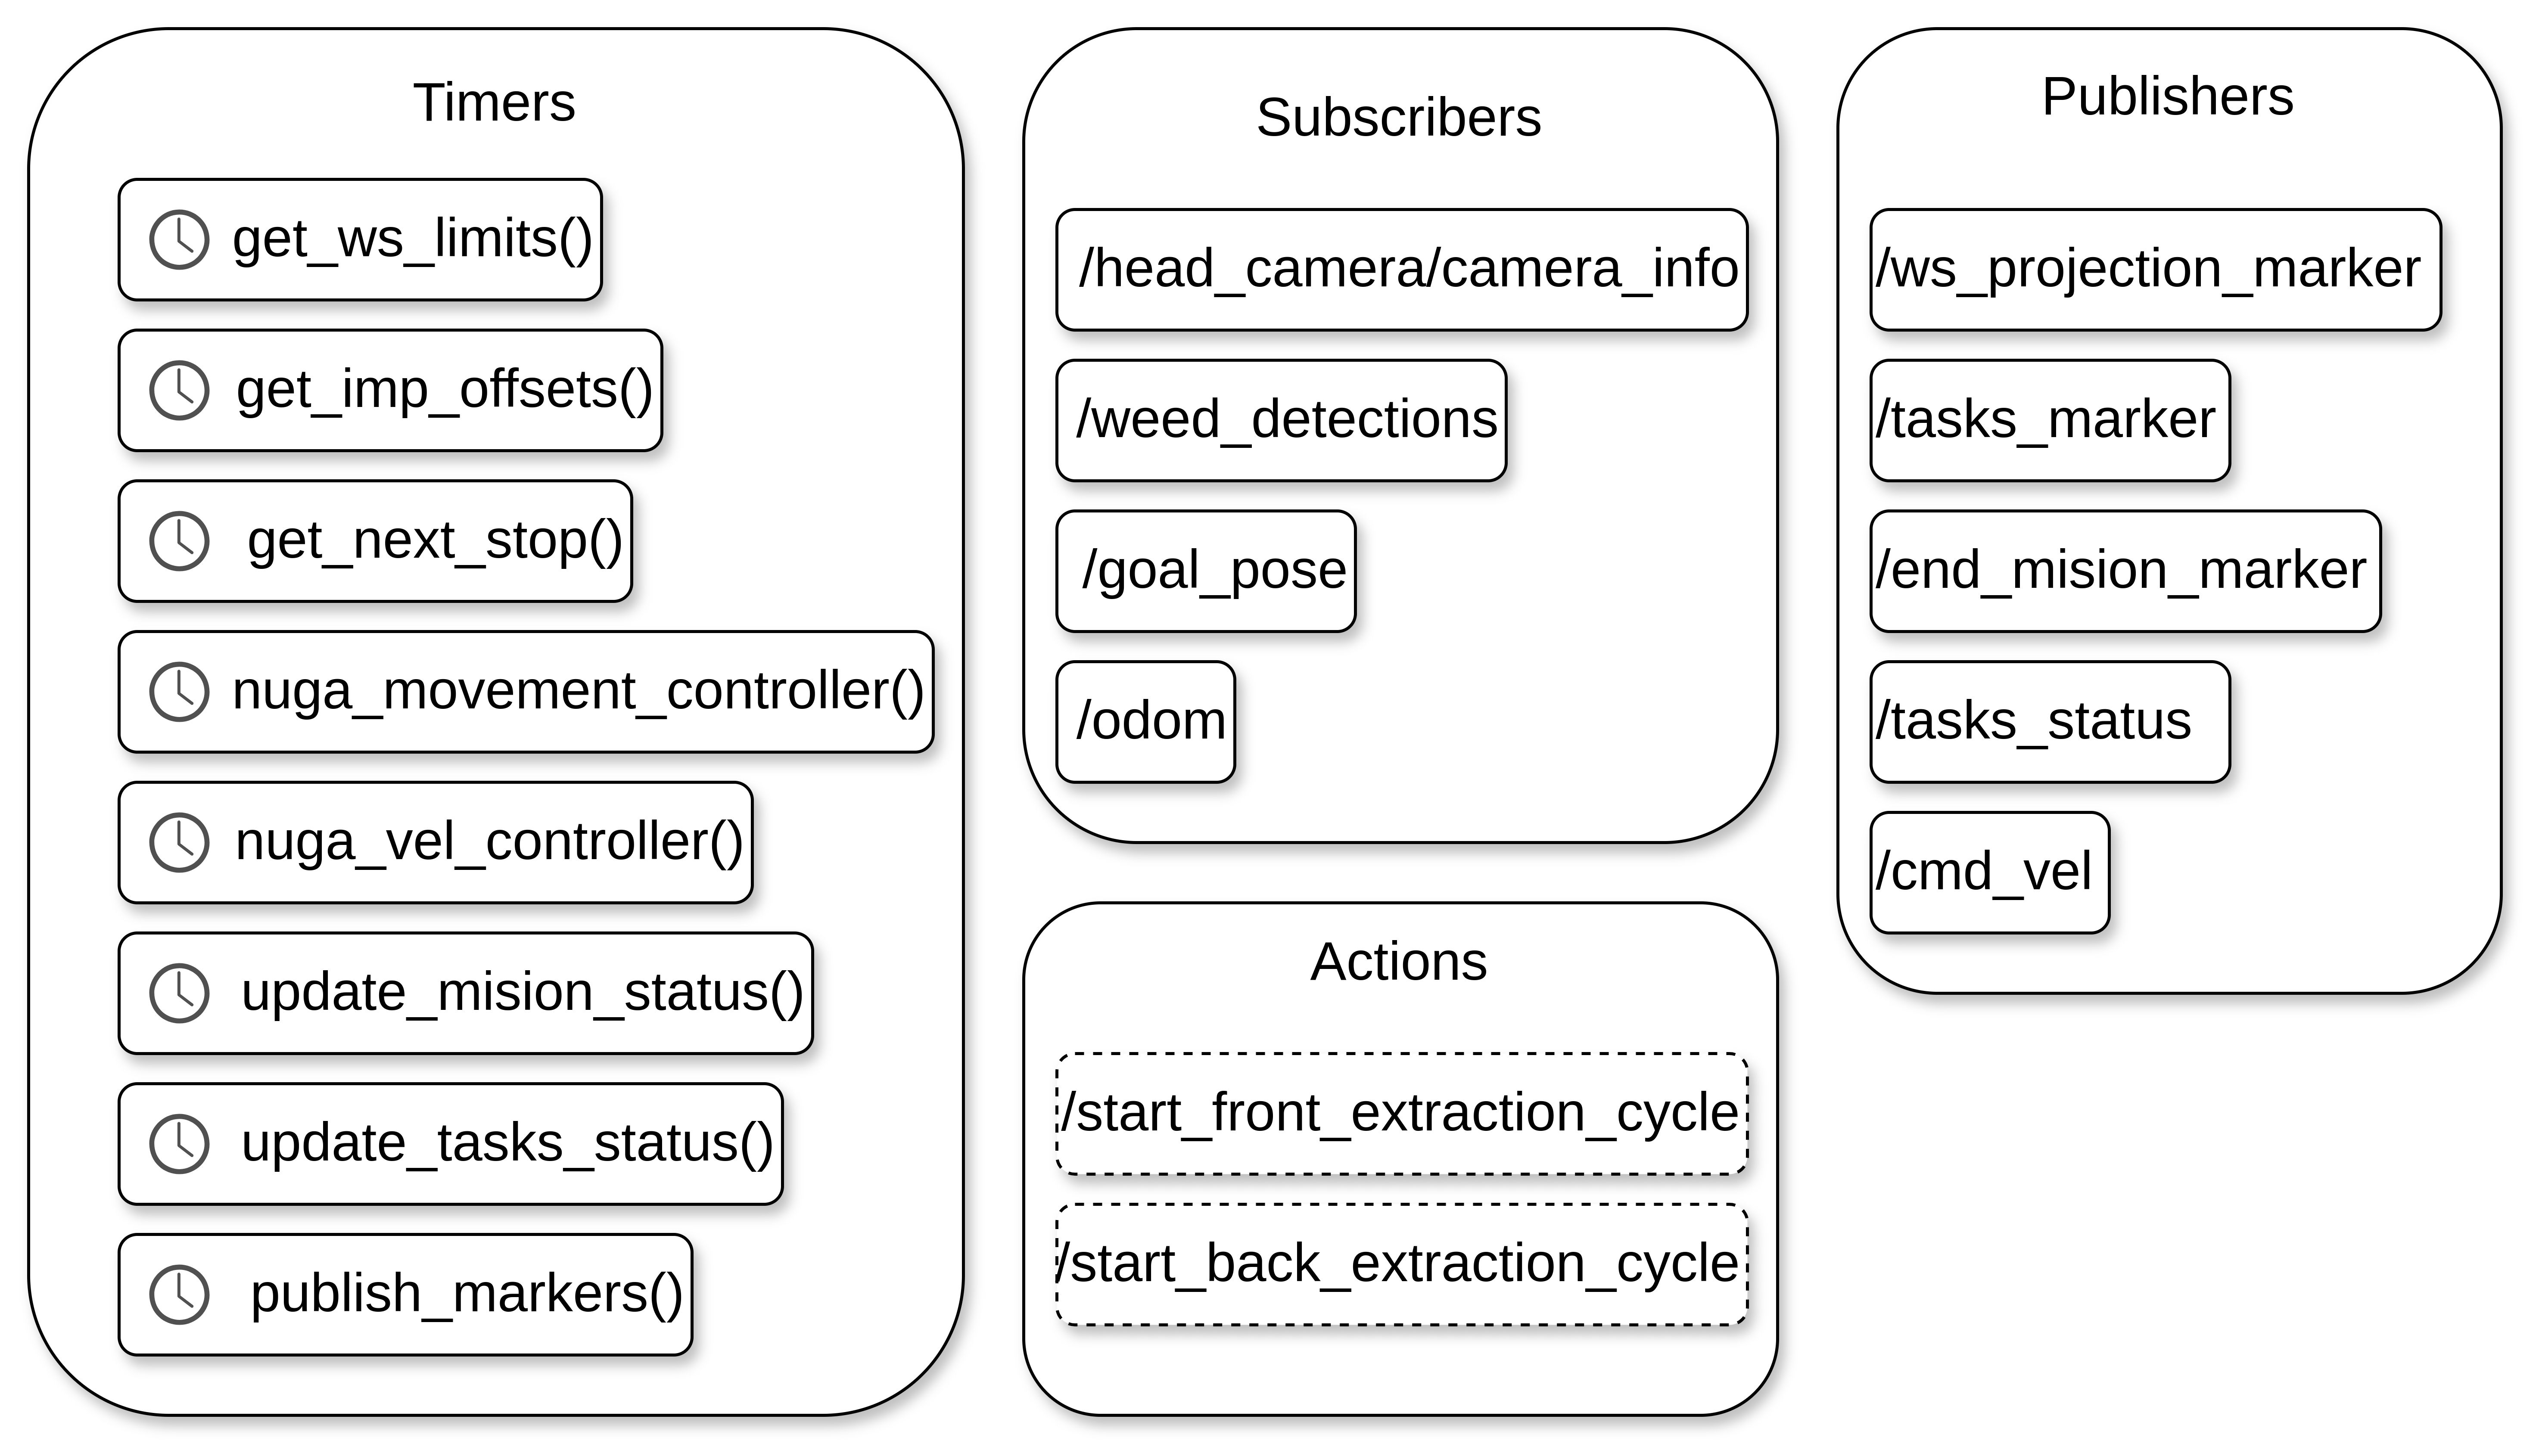
\includegraphics[width=0.95\linewidth]{gfx/ch02/nuga_controller.png}
    \caption{Nuga Controller ROS Interface}
    \label{fig:nuga-controller}
\end{figure}

The \texttt{get\_next\_stop()} function is a timer callback that computes the robot's next stop when required. It uses the current detections, the robot's pose, and the selected task allocation algorithm to determine the next target position, as well as the tasks to be executed at that stop by each \ac{IT}. The execution steps followed by this method are shown in Algorithm \ref{alg:get-next-stop}.

Once a stop is determined, Nuga’s movement and velocity controllers govern the robot’s behavior. The \texttt{nuga\_movement\_controller()} function switches the robot’s state between \textit{stationary} and \textit{moving}, while also measuring the time spent in each state. If the robot reaches the target position, this method triggers the actions required to perform the extraction cycle; otherwise, it keeps the robot in the \textit{moving} state. Finally, \texttt{nuga\_velocity\_controller()} takes the robot’s state and computes the necessary velocity commands, publishing them to the \textit{/cmd\_vel} topic.



%*****************************************
%*****************************************
%*****************************************
%*****************************************
%*****************************************

\cleardoublepage
% \ctparttext{You can put some informational part preamble text here.
% Illo principalmente su nos. Non message \emph{occidental} angloromanic
% da. Debitas effortio simplificate sia se, auxiliar summarios da que,
% se avantiate publicationes via. Pan in terra summarios, capital
% interlingua se que. Al via multo esser specimen, campo responder que
% da. Le usate medical addresses pro, europa origine sanctificate nos se.}
% \part{The Showcase}\label{pt:showcase}
% \include{Chapters/Chapter92}
%\addtocontents{toc}{\protect\clearpage} % <--- just debug stuff, ignore
%************************************************
\chapter{Task Allocation and Optimization}\label{ch:TA} % $\mathbb{ZNR}$
%************************************************
 Solving the \ac{TA} problem in this context means assigning weed detections to removal tools in the most efficient way. The idea is to find the best allocation of resources and the optimal sequence of stops, that will maximize the number of plants removed, and minimize the tools' idle time. The solution has to consider the constraints of the problem such as:

\begin{description}
    \item[Geometric Constraints:] A stop is considered valid only if the weeds lie within the workspaces of the tools (observe \autoref{fig:problem-layout.png}).
    \item[Movement Constraints:] The robot can only move forward in a straight line at a max speed of $0.3\frac{m}{s}$. % acceleration and deceleration times have to be considered.
    \item[Task Processing:] Each plant removal takes approximately $45$ seconds, during which the robot must remain stationary to ensure a successful extraction. Movement during this process is not allowed as it could compromise the tool operation.
    \item[Dynamic Environment:] Weed positions are initially unknown and are discovered dynamically during operation by the camera in front of the vehicle.
    \item[Processing Time:] The solution must run online because the robot discovers new weeds during operation, and decisions about stopping and \ac{TA} must adapt in real-time.
\end{description}

We define a '\textit{good}' stop as the next robot position that maximizes plant coverage while keeps a balance on the number of tasks assigned to each implement (aiming to minimize idle time). The problem can be approached in two ways: one option is to first determine the optimal stop location, after which task allocation becomes trivial by simply assigning tasks based on whether they fall within the front or back workspace. Alternatively, we can first allocate tasks to the implements and then compute the stop position that satisfies the corresponding geometric constraints. Both approaches are similar, differing mainly in the order of operations, but each perspective opens the door to different methods and algorithms to try.

\begin{figure}[bth]
    \centering
    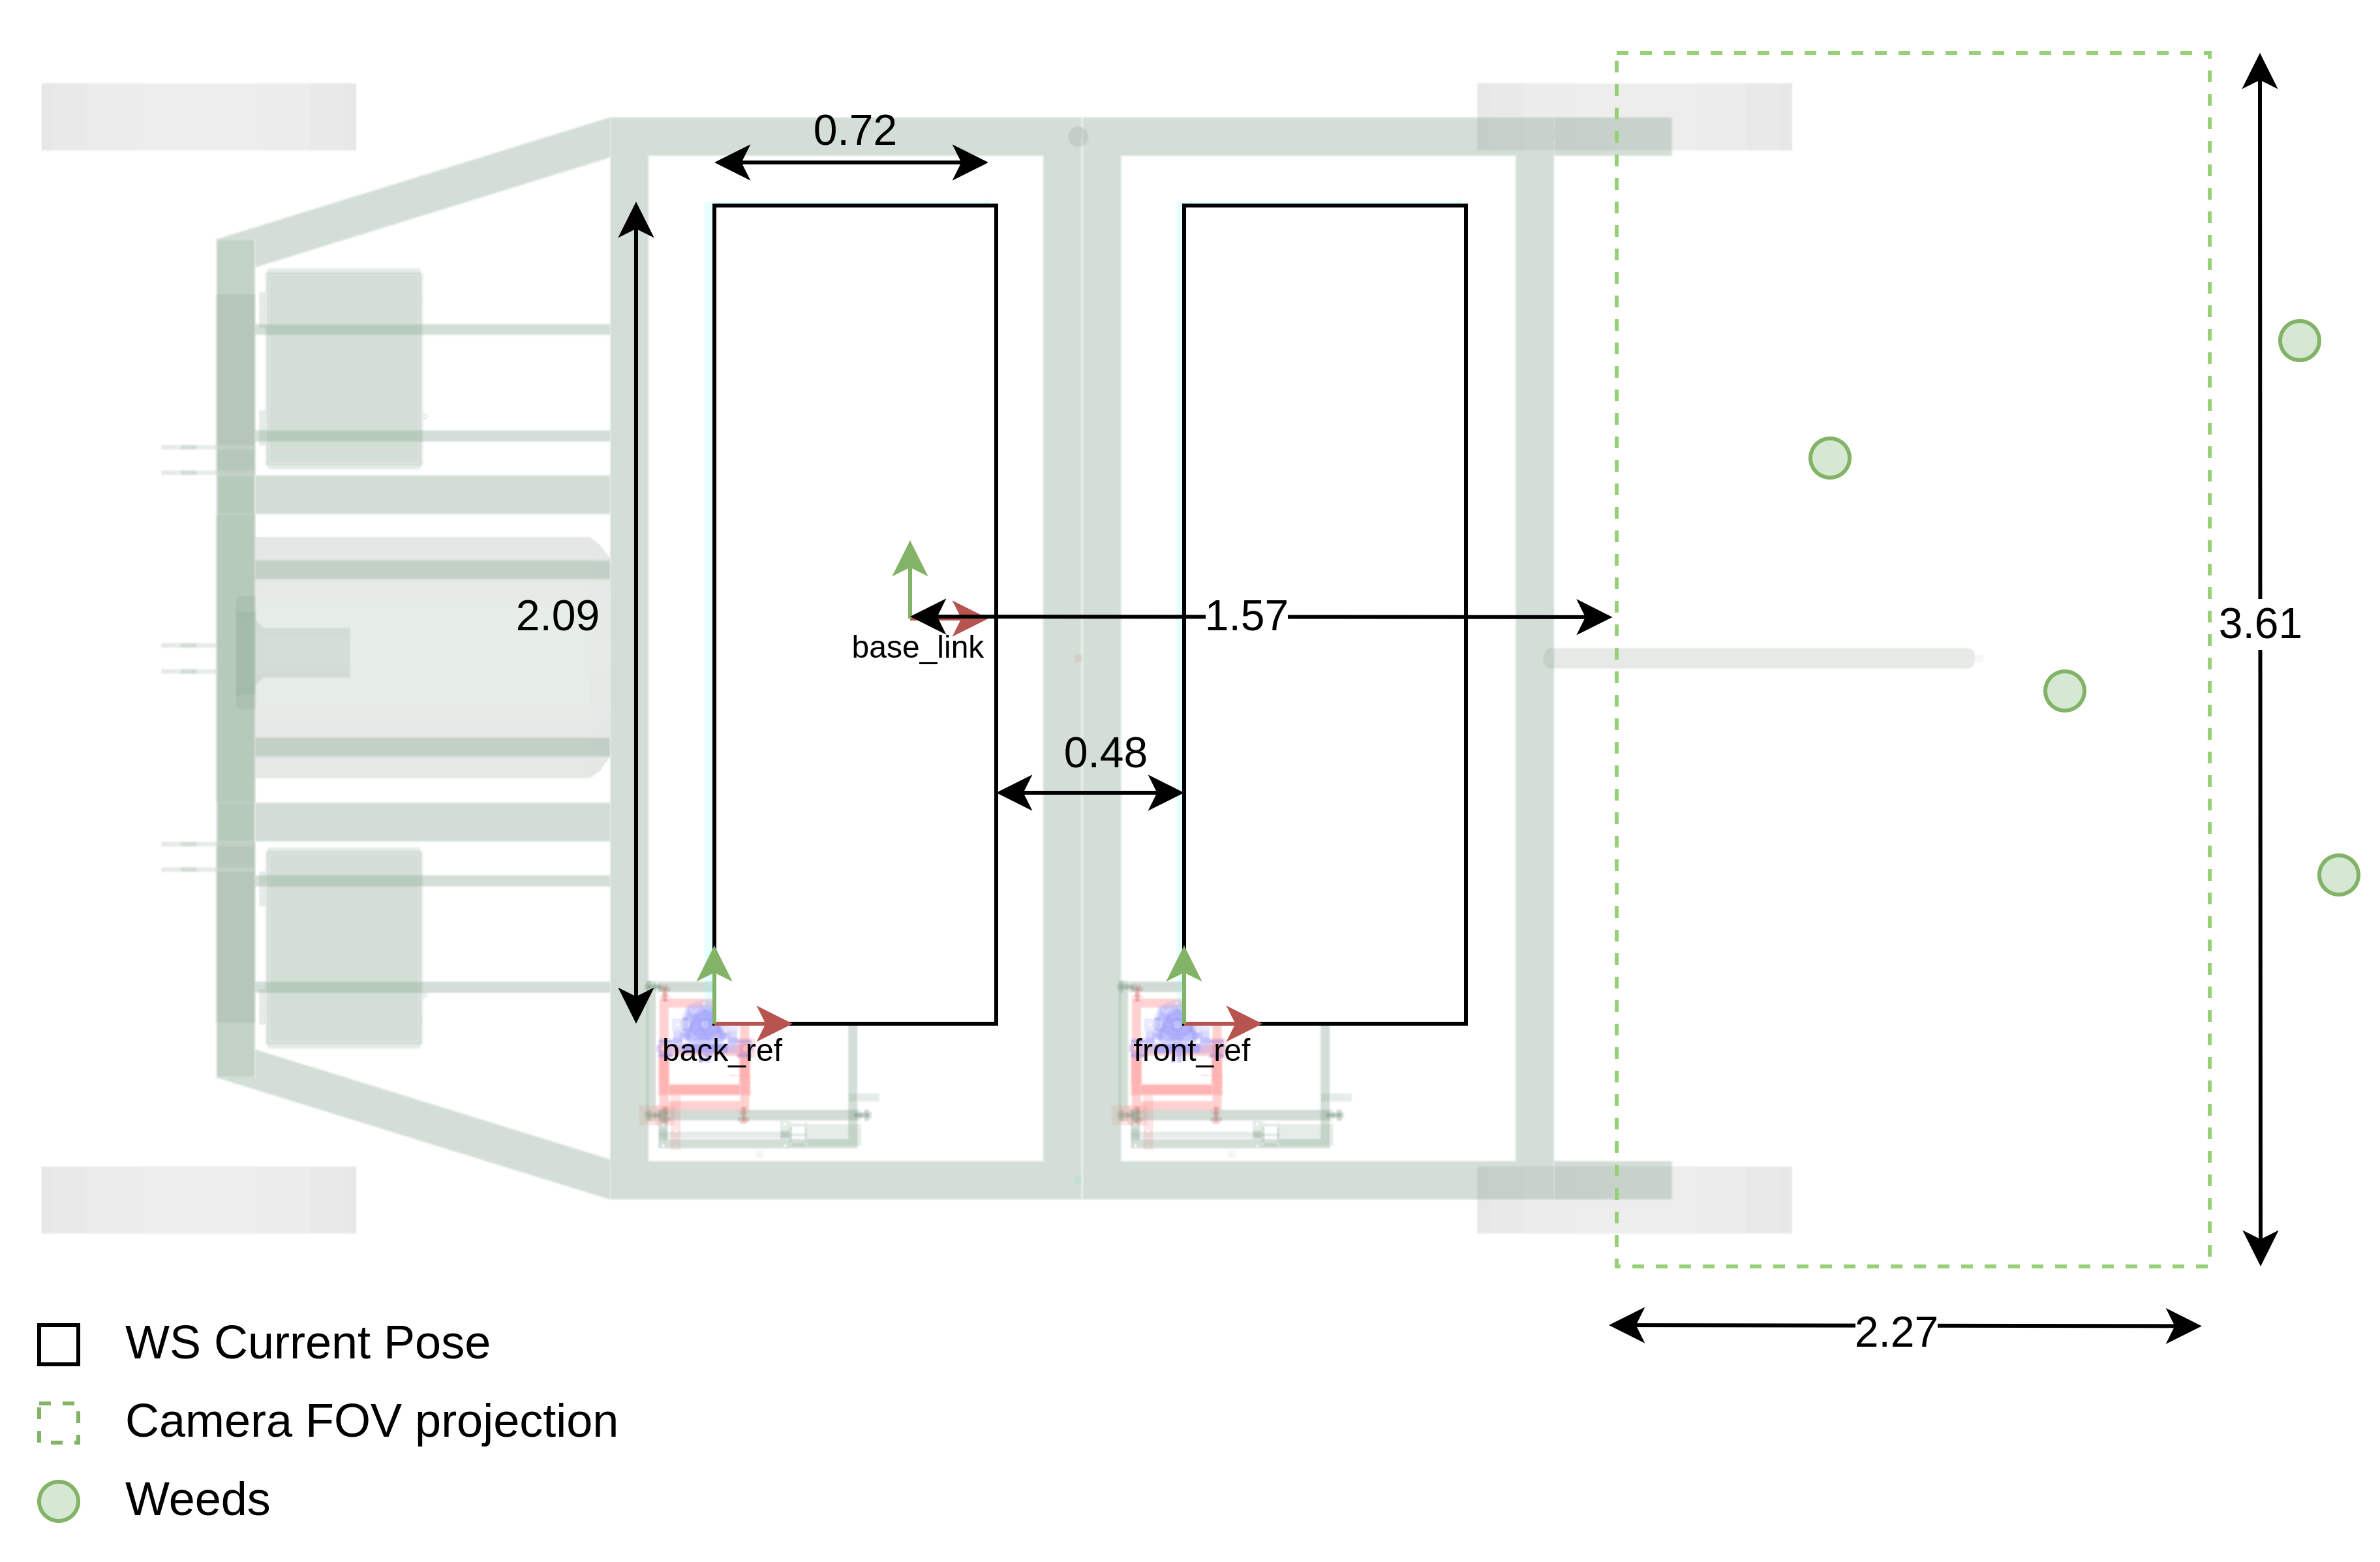
\includegraphics[width=\linewidth]{gfx/ch03/problem_layout.png}
    \caption{Problem Layout Dimentions}
    \label{fig:problem-layout.png}
\end{figure}

\section{Metrics}
Defining a good set of metrics is crucial to establish a solid basis for comparison between solutions and to easily identify the flaws of each method, thereby determining the best solution. To address this, we define two main categories. The first summarizes mission-level metrics such as the total idle and productive time of each tool, and the total time the robot spends moving or in a stationary state (defined by equations \ref{eq:total-mission-time} and \ref{eq:tool-usage-time}). The second category includes task-specific information, for example, task ID, status ('\textit{compleated}', '\textit{failed}', '\textit{out}'), number of stops, the tool that processed the task, and the idle and productive time of each tool at that specific stop. These metrics are displayed in a mission dashboard for easy visualization and comparison across missions using different worlds or algorithms (see \autoref{fig:mission-metrics} for the first category and \ref{fig:task-metrics} for the second one).

\begin{figure}[htb]
    \myfloatalign
    \subfloat[Mission Category Metrics]
    {\label{fig:mission-metrics}
        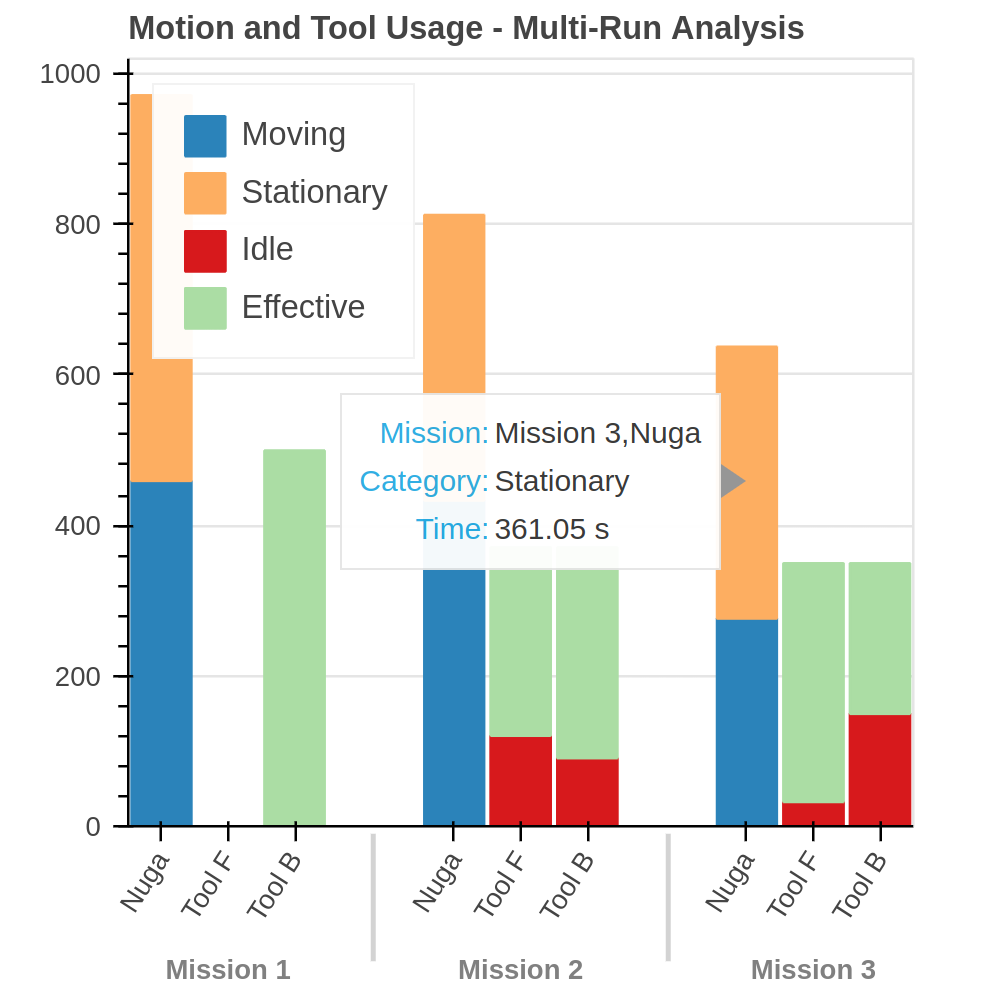
\includegraphics[width=.45\linewidth]{gfx/ch03/mission_metrics.png}} \quad
    \subfloat[Task Visualization]
    {\label{fig:task-metrics}%
        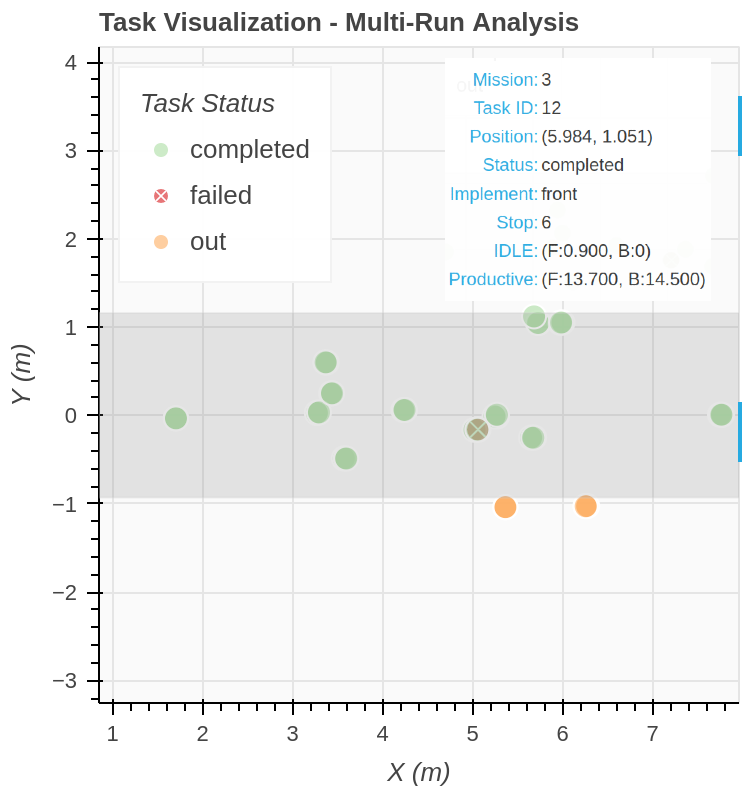
\includegraphics[width=.45\linewidth]{gfx/ch03/task_metrics.png}} \\
    \caption{Mission Dashboard}\label{fig:mission-dashboard}
\end{figure}


\paragraph{\autoref{fig:mission-metrics}} Showcases a bar graph comparing different missions. Each mission includes the robot's moving and stationary time, as well as the idle and productive time of the onboard implement tools. A hover feature displays the value of each category.

\paragraph{\autoref{fig:task-metrics}} Displays a 2D grid of the removed tasks' positions during the mission, along with their corresponding metadata. Hovering over a task reveals its details, and tasks can be filtered by mission.

\begin{equation}
    t_{mission} = t_{moving} + t_{stationary}
\label{eq:total-mission-time}
\end{equation}

\begin{equation}
    t_{tool\_operation} = t_{idle} + t_{productive}
\label{eq:tool-usage-time}
\end{equation}


\section{Heuristics}
Heuristic solutions are commonly employed when the solution space of an optimization problem is too large to explore exhaustively, making an exact optimal solution computationally infeasible. They are also useful in time-sensitive scenarios, such as online implementations, where sacrificing optimality for efficiency is often justified.

In our work, we developed a heuristic algorithm to serve as a baseline solution, this provides a meaningful reference point to assess the performance and potential improvements offered by other algorithms. The algorithm' description is detailed in \ref{alg:heuristic}, with an illustrative example in \autoref{fig:heuristic-steps}.

\begin{algorithm}
    \caption{Heuristic}
    \begin{algorithmic}[1]
        \STATE Get the position of the closest weed from the current robot position.  
        \STATE Project the tools' \ac{WS} forward (in the future), aligning the trailing edge of the last \ac{WS} with the closest weed's position plus a small clearance (e.g., 10 cm).  
        \STATE Allocate weeds to each tool if they fall within its projected \ac{WS}.
        \STATE Move the robot until the tools' \ac{WS} are aligned with their projections, then execute the extractions for tools with assigned weeds.  
        \STATE Repeat the process until mission has ended.  
    \end{algorithmic}
    \label{alg:heuristic}
\end{algorithm}

\begin{figure}[htb]
    \myfloatalign
    \subfloat[S1.Closest task, S2.WS projection]
    {\label{fig:heuristic-s1-s2}
        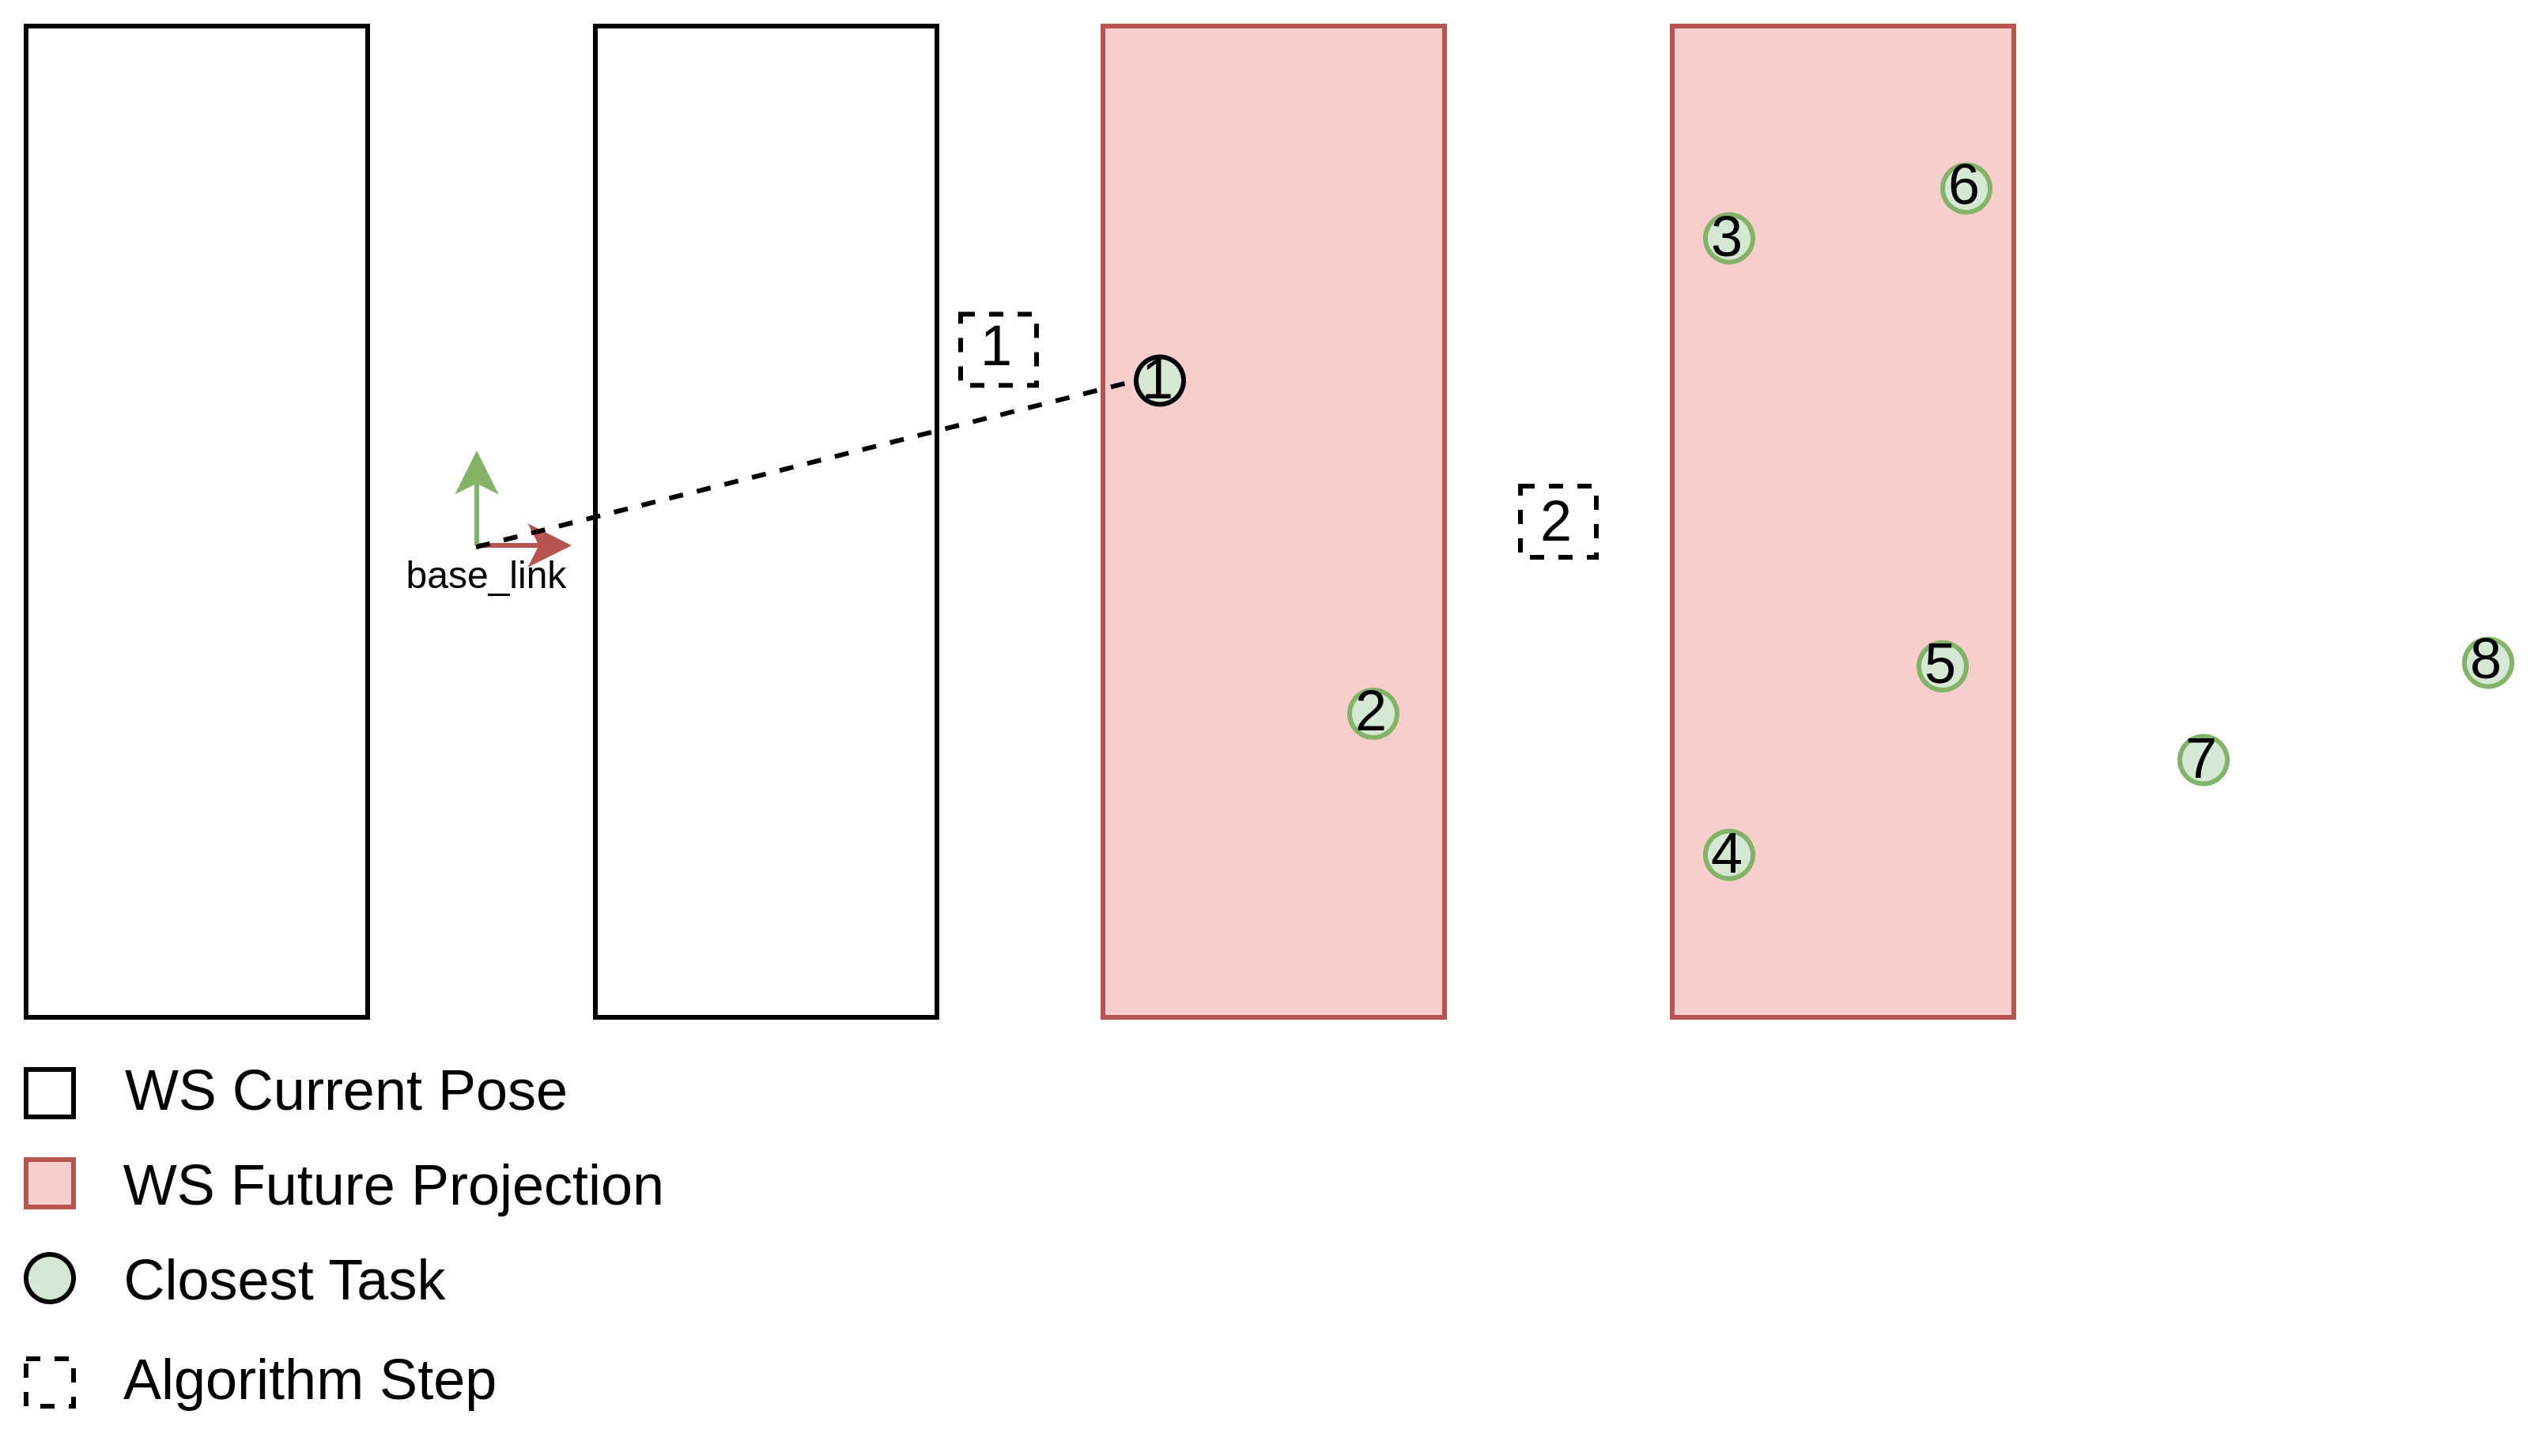
\includegraphics[width=.50\linewidth]{gfx/ch03/heuristic_s1_s2.png}} \quad
    \subfloat[S3.Task Allocation]
    {\label{fig:heuristic-s3}%
        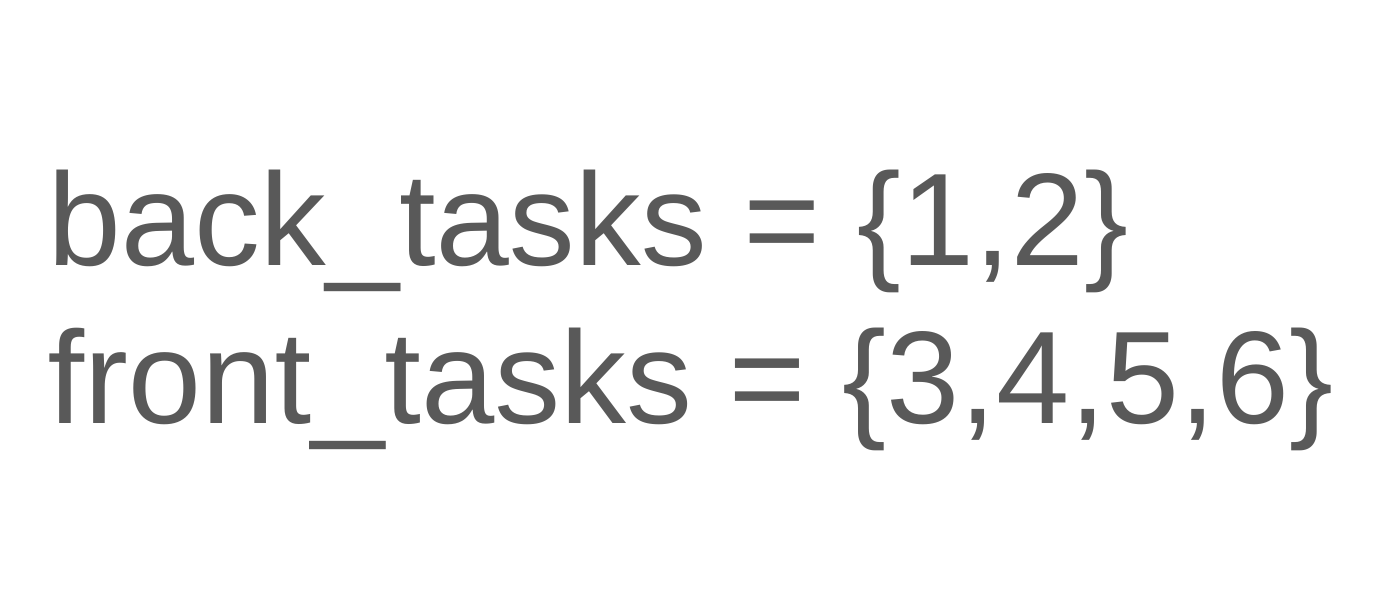
\includegraphics[width=.40\linewidth]{gfx/ch03/heuristic_s3.png}} \\
    \subfloat[S4.Moving until aligned and extraction]
    {\label{fig:heuristic-s4}
        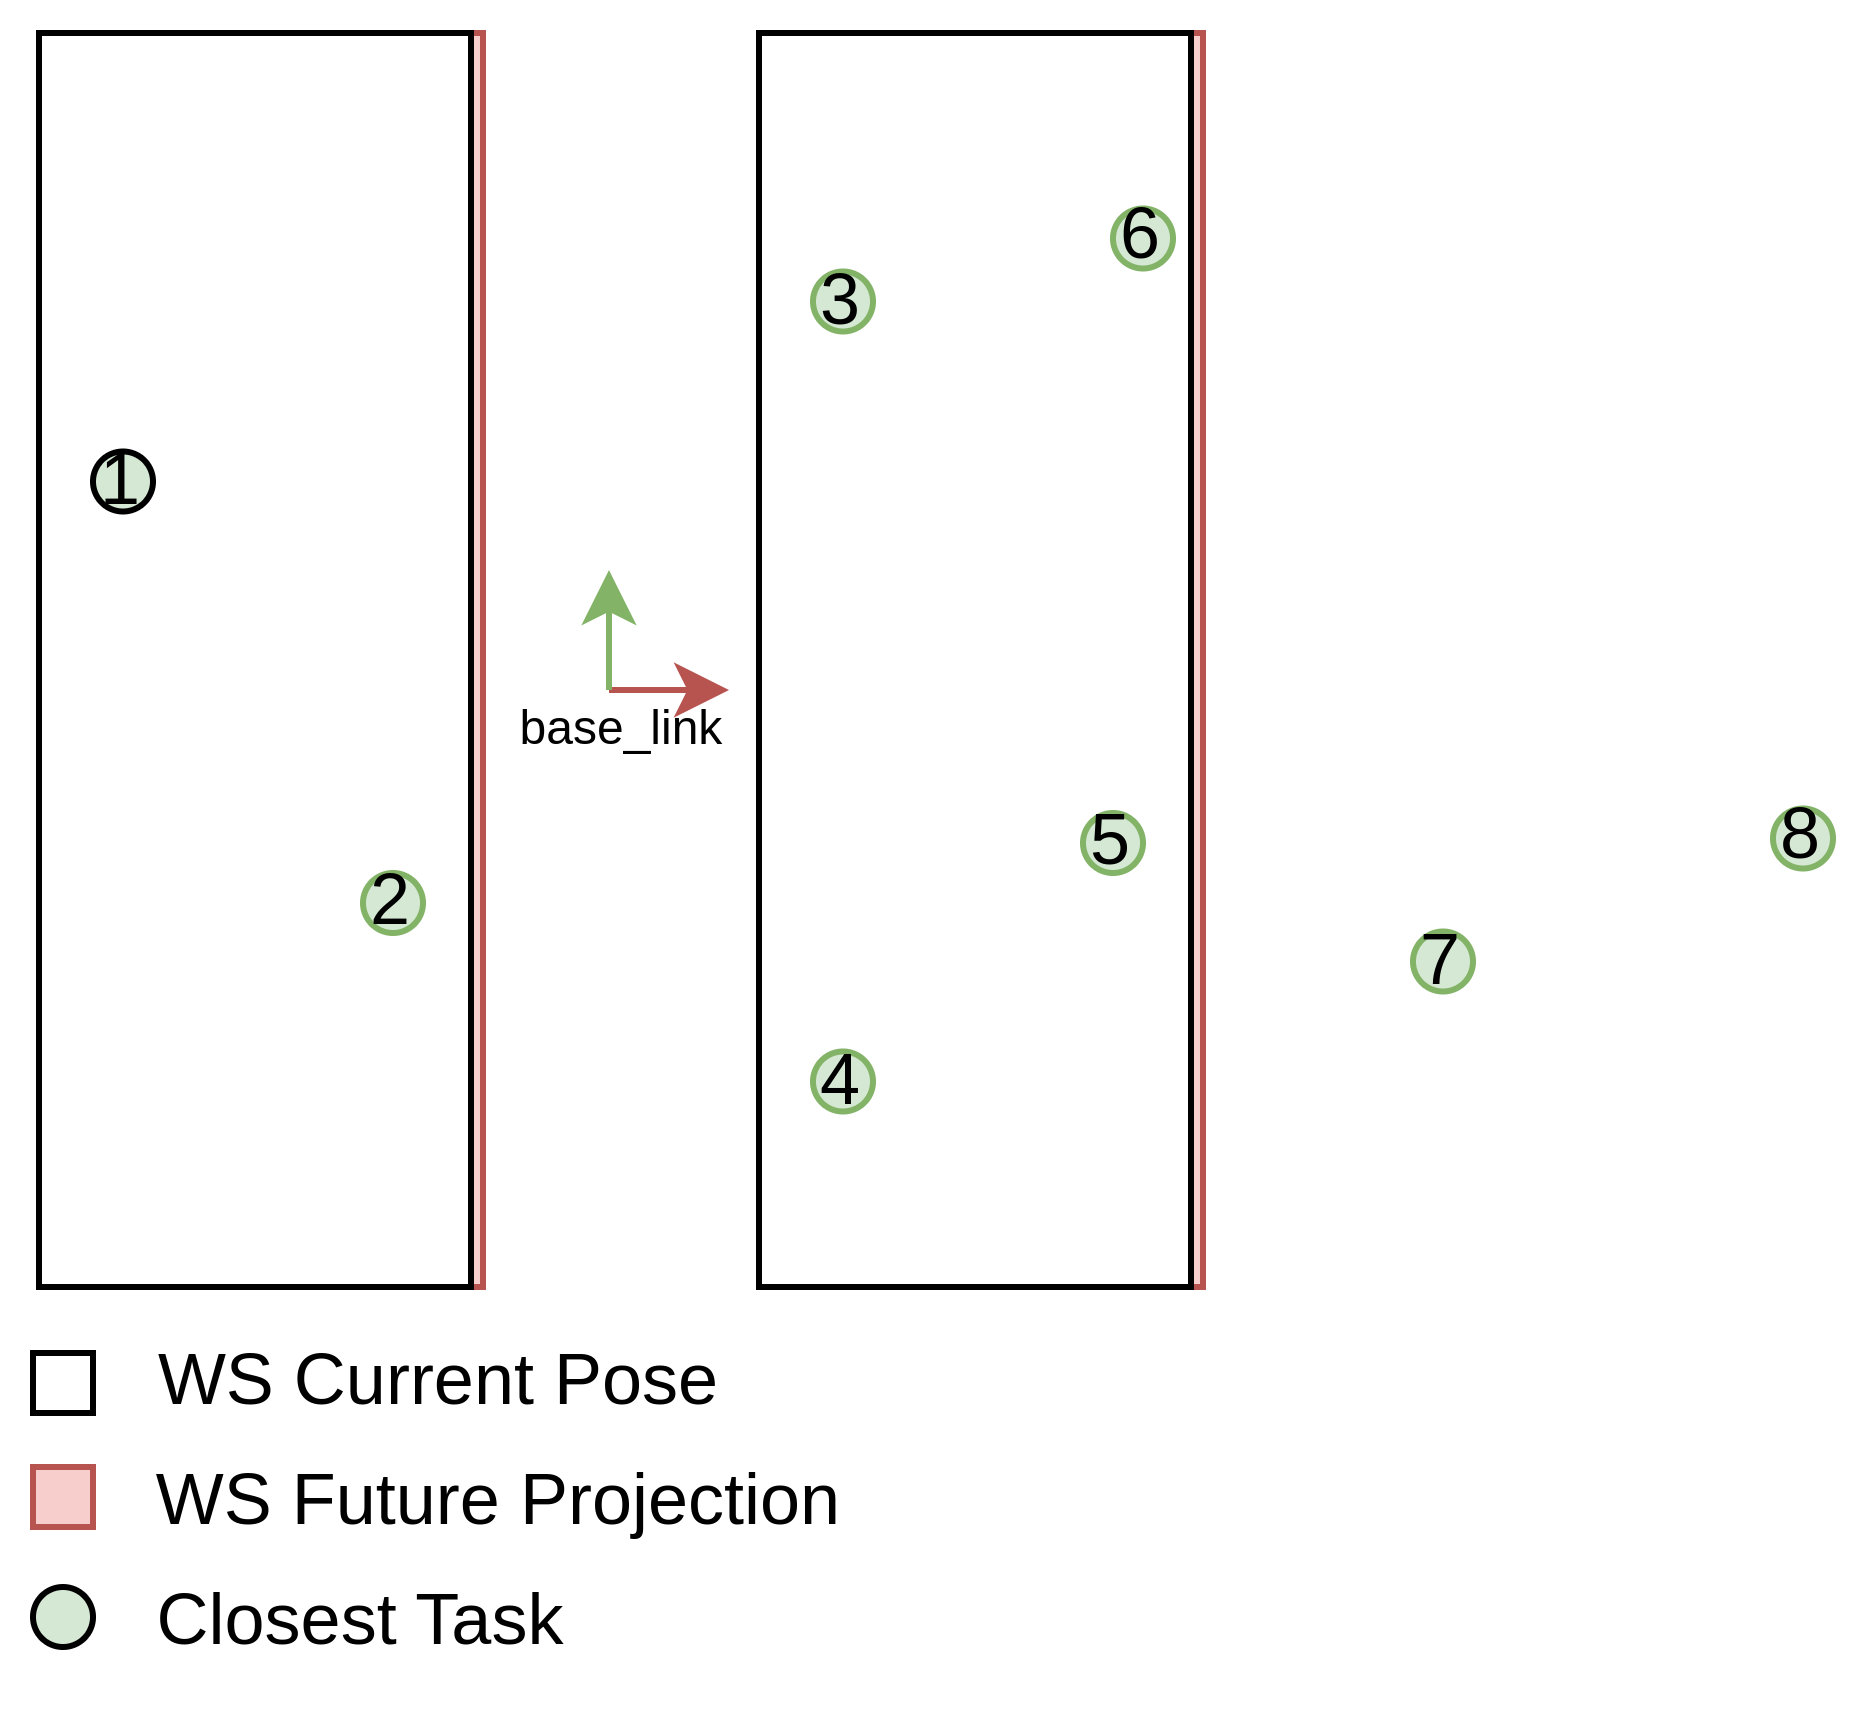
\includegraphics[width=.40\linewidth]{gfx/ch03/heuristic_s4.png}} \quad
    \subfloat[S5.Repeat]
    {\label{fig:heuristic-s5}%
        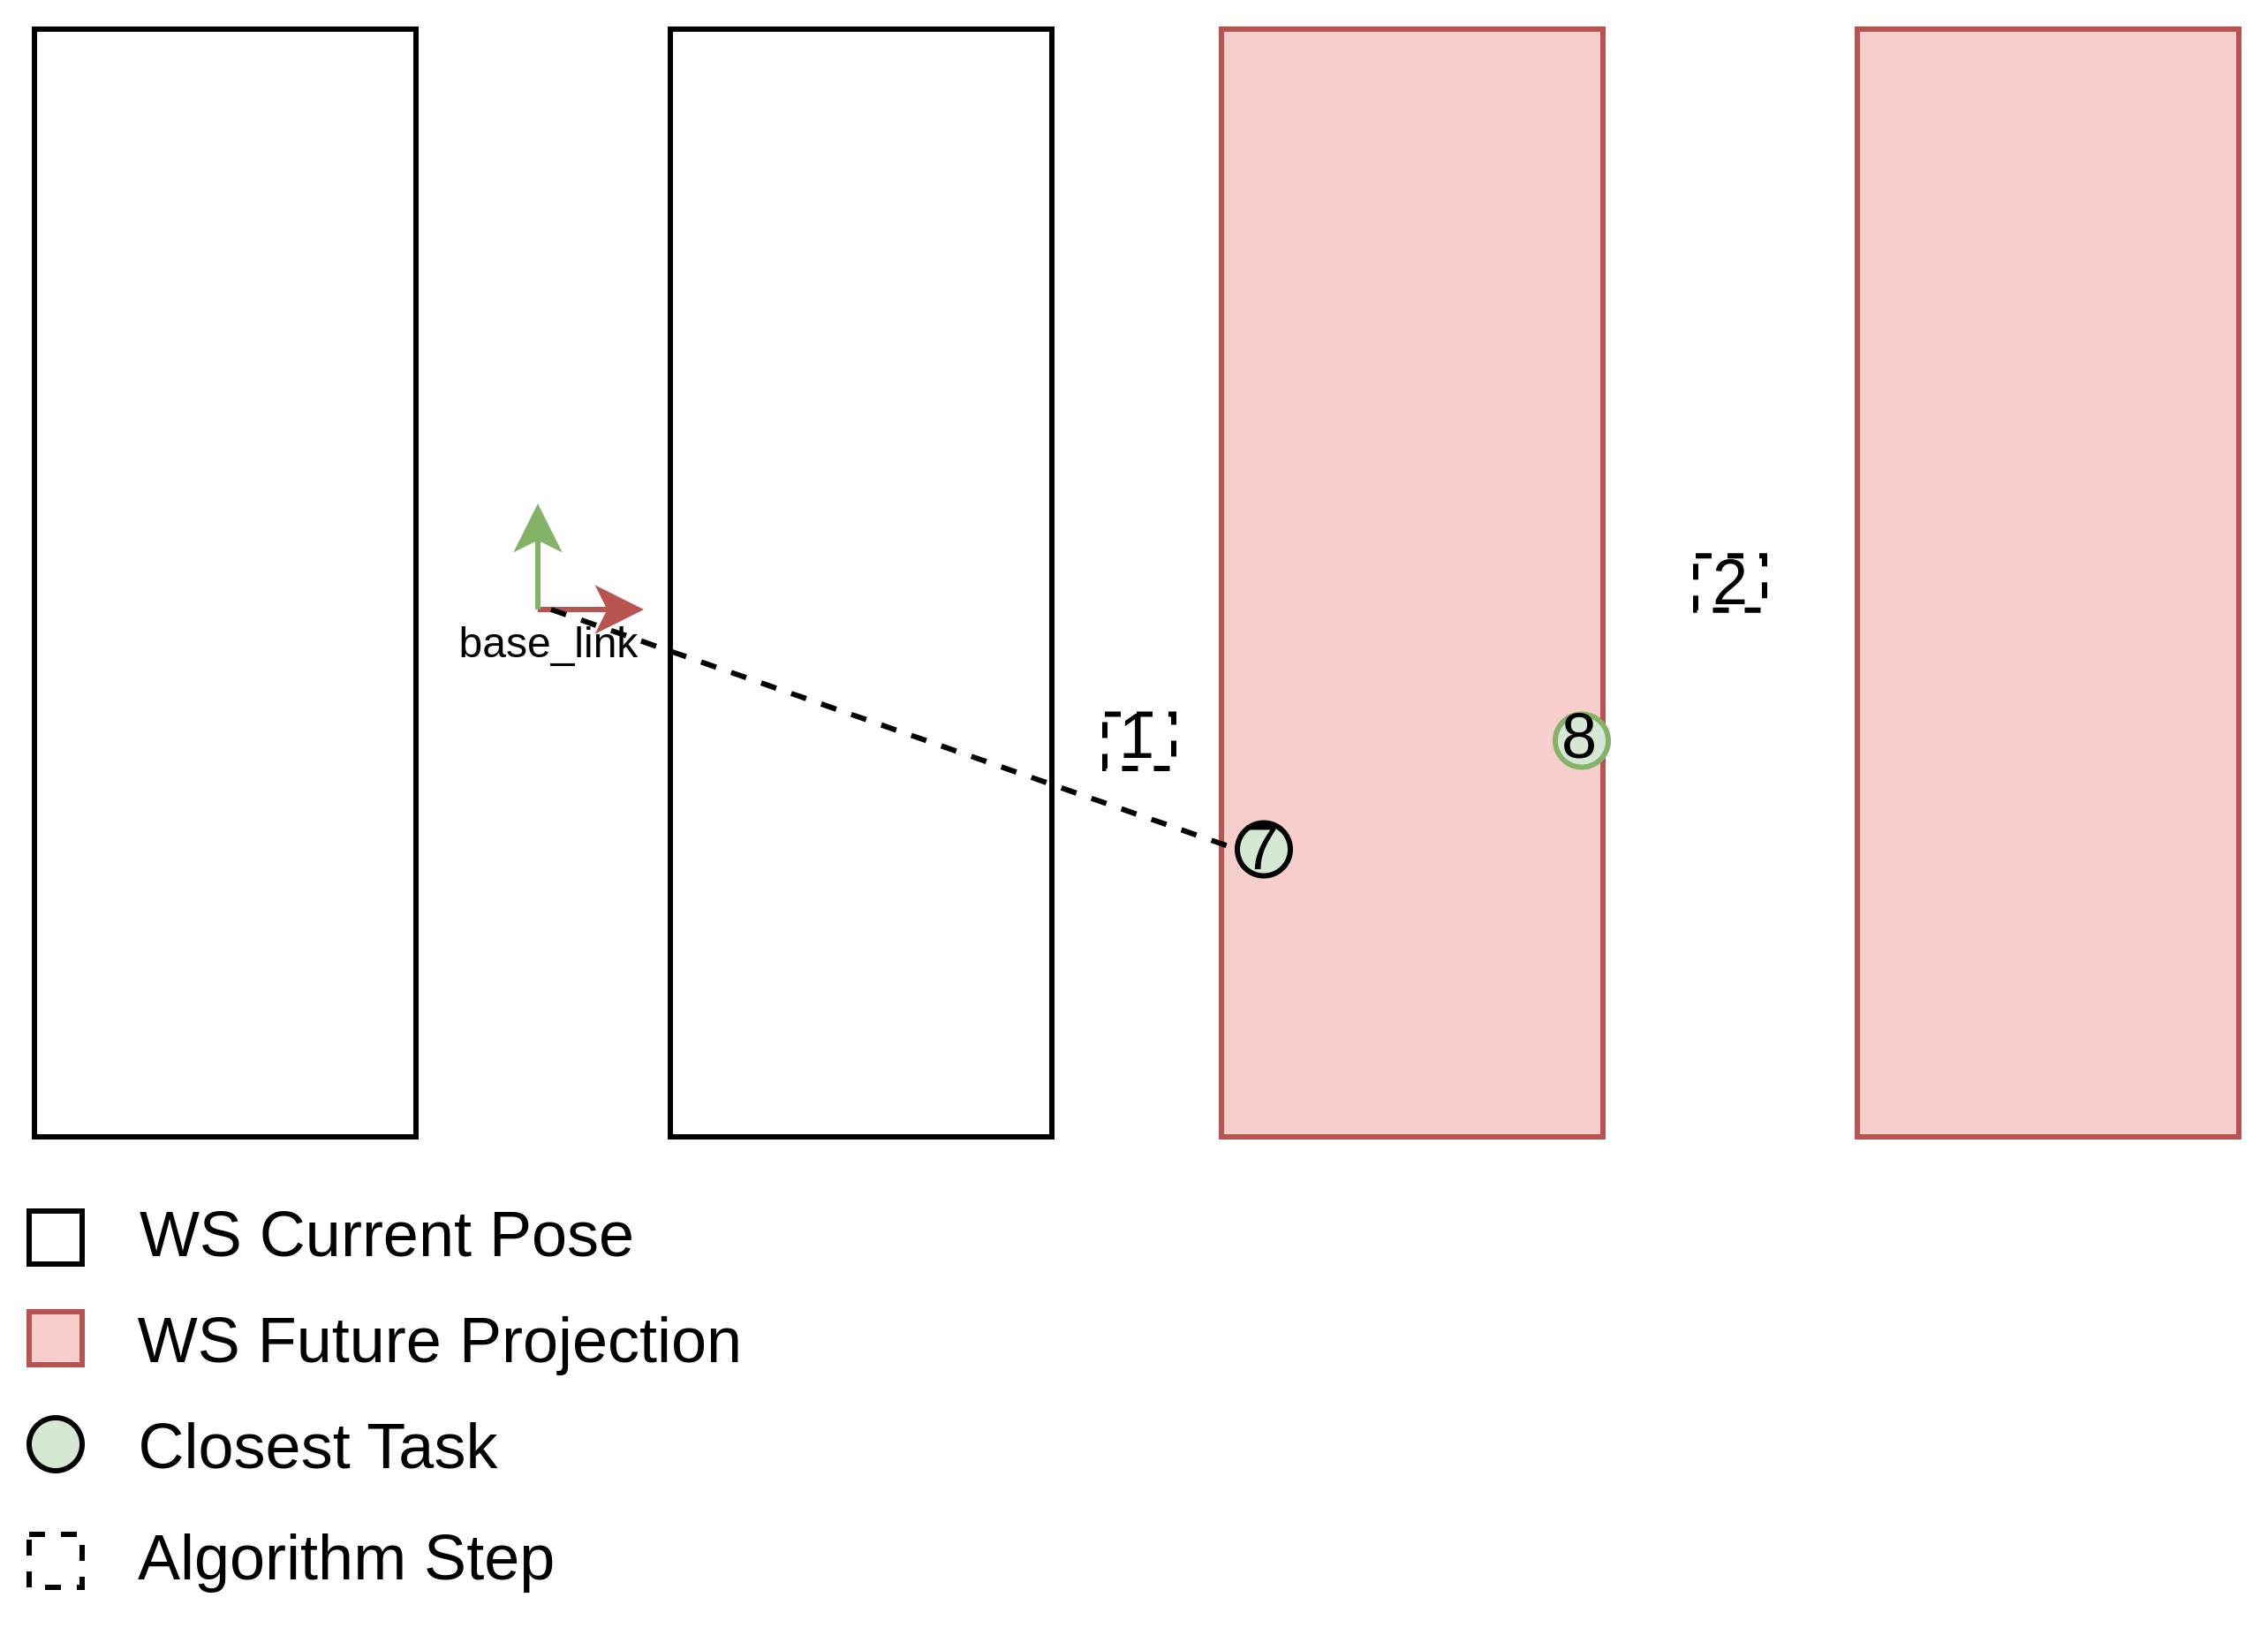
\includegraphics[width=.50\linewidth]{gfx/ch03/heuristic_s5.png}} \\
    \caption{Heuristic Algorithm}\label{fig:heuristic-steps}
\end{figure}

This approach offers a simple implementation and fast computation solution, making it well-suited for online applications. However, its heuristic nature leads to suboptimal solutions, as it does not account for minimizing idle time. In \autoref{fig:heuristics-suboptimal} we exemplify the algorithm' suboptimality for a particular case, contrasting with a better solution to support our analysis.

\paragraph{\autoref{fig:heuristic-suboptimal-stops}} Showcases the two stops required to remove eight weed' detections, with the first stop allocating four tasks to the back tool and the second stop allocating two tasks to the front tool.

\paragraph{\autoref{fig:heuristic-suboptimal-time}} Illustrates the idle and productive time for the given solution. Blue represents the robot’s repositioning time, red indicates the idle time of the respective tool, and white the productive time. The first stop shows a significant idle time for the front tool (90 seconds, equivalent to two tasks), caused by the tool waiting for the back tool to finish before proceeding to the next stop. The second stop shows a similar situation, where idle time arises from the only feasible option at that point: removing tasks 5 and 6 with the back tool.

\begin{figure}[htb]
    \myfloatalign
    \subfloat[Two stops required]
    {\label{fig:heuristic-suboptimal-stops}
        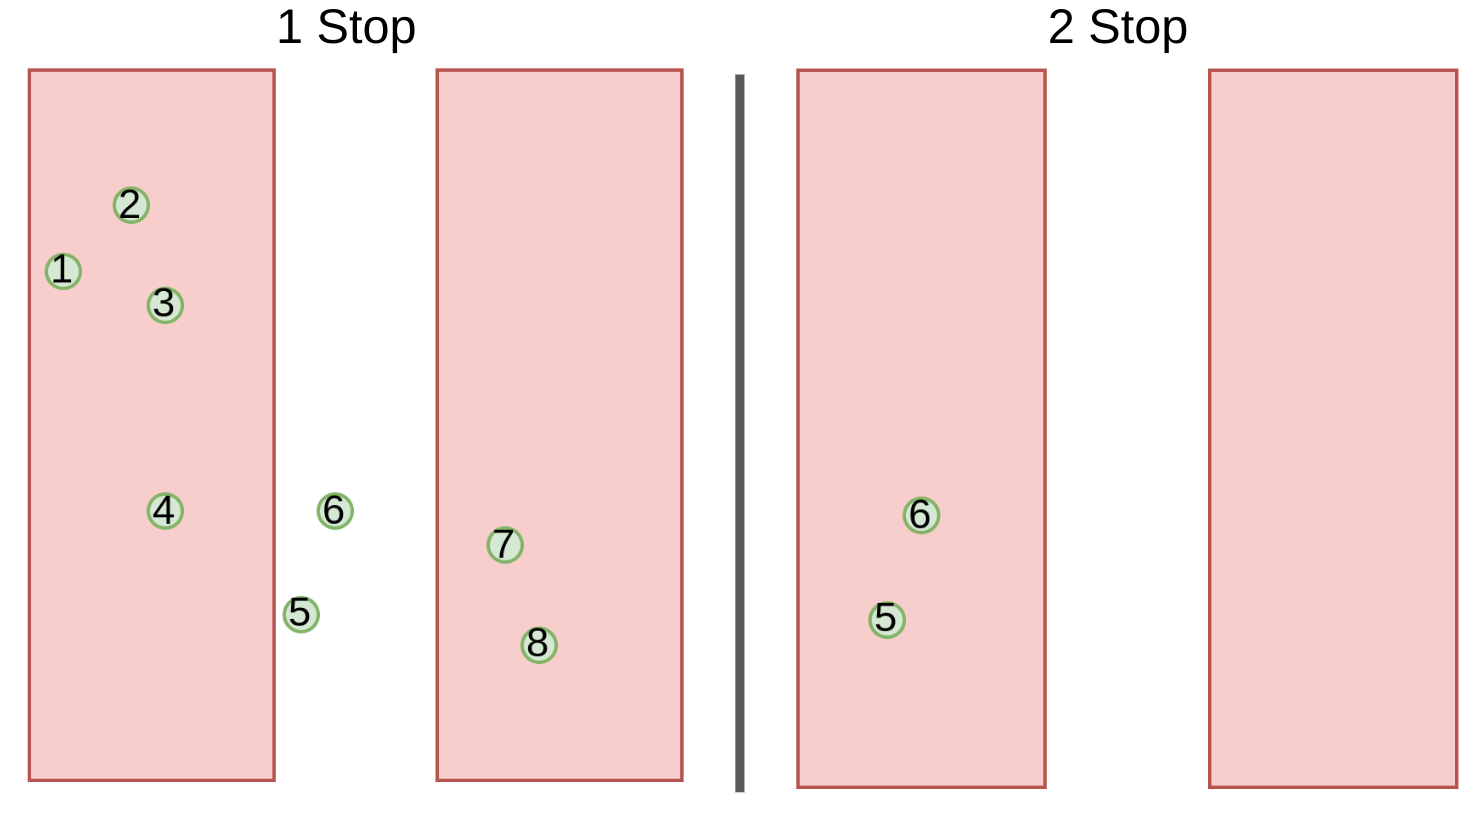
\includegraphics[width=0.6\linewidth]{gfx/ch03/heuristic_suboptimal_stops.png}}

    \subfloat[Idle and productive time of each tool]
    {\label{fig:heuristic-suboptimal-time}
        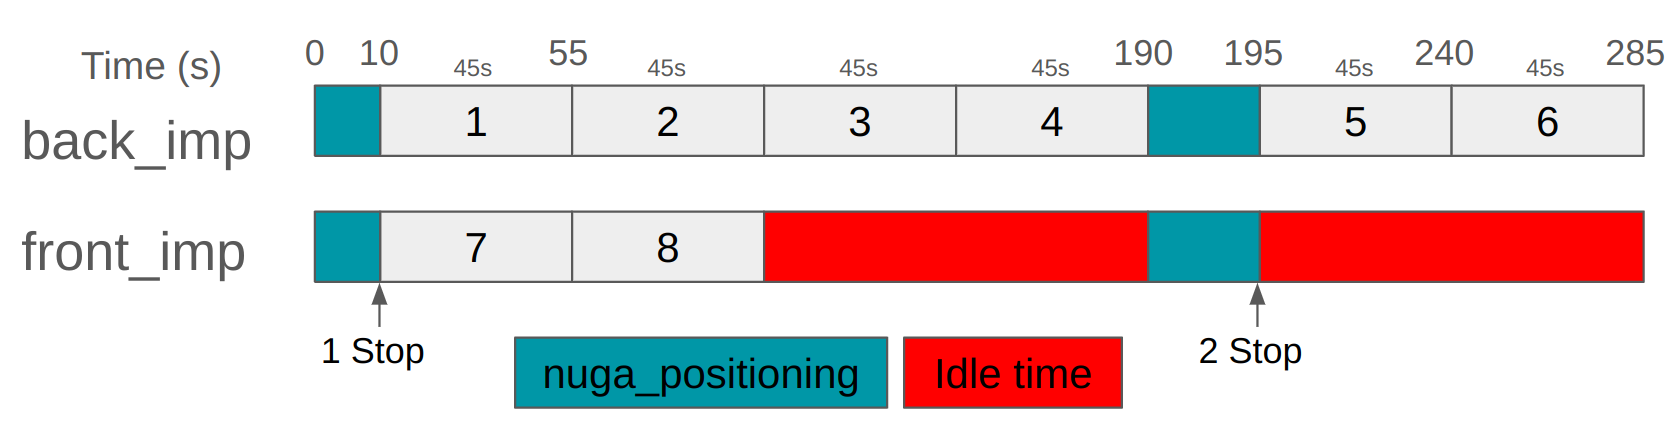
\includegraphics[width=0.9\linewidth]{gfx/ch03/heuristic_suboptimal_time.png}}

    \caption{Suboptimal solution computed using Heuristic}
    \label{fig:heuristics-suboptimal}
\end{figure}

An alternative solution for the same scenario (this time aimed at reducing idle time) is illustrated in \autoref{fig:heuristics-optimal}. In this case, the solution requires three stops: first stop assigns tasks 1 to back tool and task 5 to the front, the second stop processes tasks 2 and 6, and finally the third stop is used to remove tasks 3, 4, 7, and 8. As shown in \autoref{fig:heuristic-optimal-time}, the balanced task allocation between tools eliminates idle time and reduces the total mission duration compared to the previous solution.

This demostrates the heuristic's suboptimality, as it fails to minimize idle time and does not consider the possibility of stopping at a location that allows for a more efficient task allocation. The heuristic algorithm is limited to the closest weed detection, which may not always be the best option. In the following sections, we will explore more sofisticated algorithms that can overcome these limitations and provide better solutions. 

\begin{figure}[hbt]
    \myfloatalign
    \subfloat[Three stops required]
    {\label{fig:heuristic-optimal-stops}
        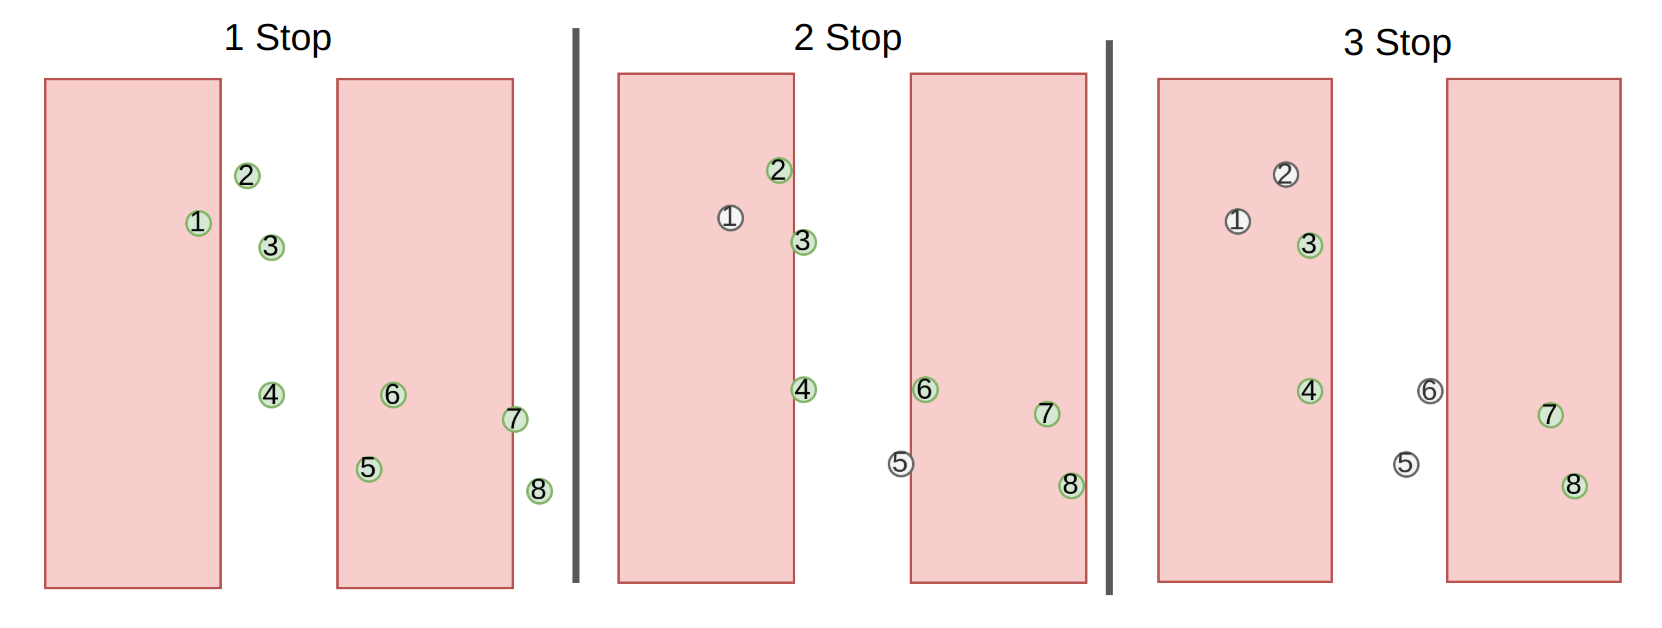
\includegraphics[width=0.6\linewidth]{gfx/ch03/heuristic_optimal_stops.png}}

    \subfloat[Idle and productive time of each tool]
    {\label{fig:heuristic-optimal-time}
        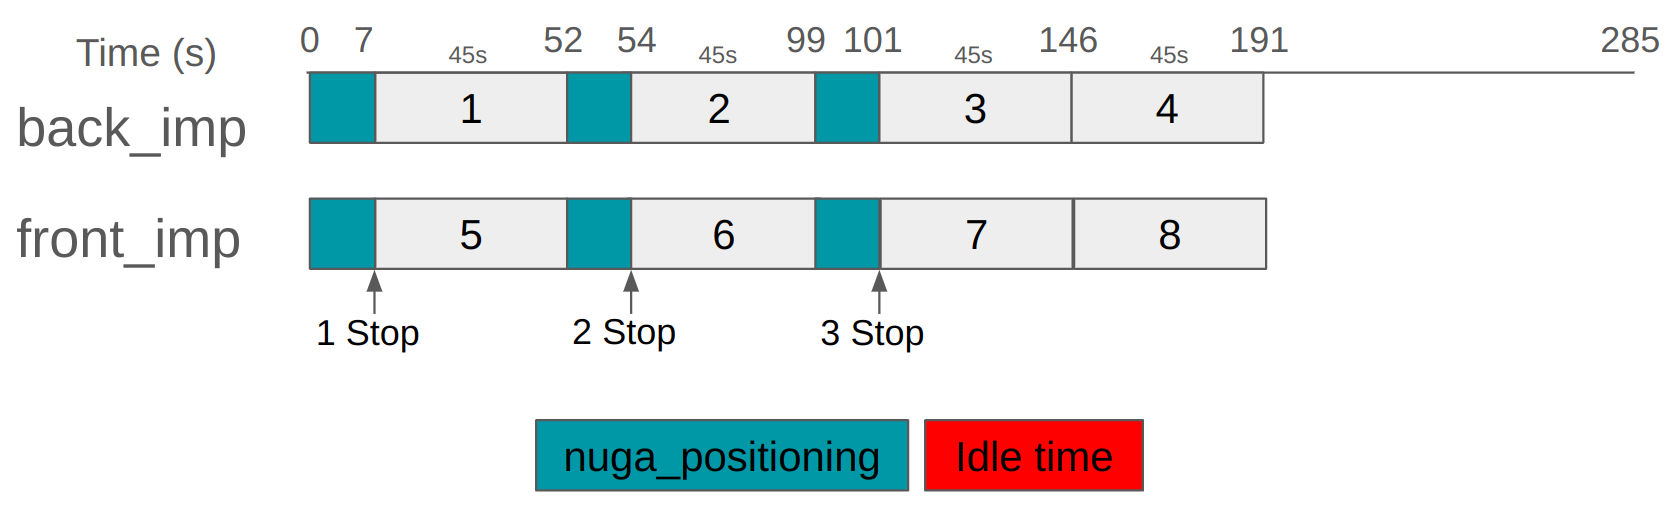
\includegraphics[width=0.9\linewidth]{gfx/ch03/heuristic_optimal_time.png}}

    \caption{Optimal solution}
    \label{fig:heuristics-optimal}
\end{figure}

\section{Graph Search}
Graph Search are a type of algorithms widely used in graph theory to systematically explore or traverse a graph. They are commonly used to find the shortest path between nodes, identify connected components, or solve various optimization problems. Graph search algorithms can be broadly categorized into two main types: uninformed and informed search algorithms.

Uninformed search algorithms do not have any additional information about the problem domain and explore the graph blindly. Examples include \ac{DFS} and \ac{BFS}. These algorithms are typically used for tasks like finding connected components or traversing all nodes in a graph.
Informed search algorithms, on the other hand, use heuristics or additional information to guide the search process. They are often more efficient than uninformed algorithms for specific problems. Examples include A* search and Dijkstra's algorithm, which are commonly used for finding the shortest path in weighted graphs.

In our context, we exploit the advantages of graph-based algorithms by modeling the problem as such. Nodes represent potential stop locations, where two types of actions are possible: moving to another stop (a \textit{stop node}) or performing weed removal at that location (an \textit{action node}). Edge weights are defined as follows: edges between two \textit{stop nodes} represent \textit{travel cost}, computed using the distance between stops and the robot’s velocity or a unitary value as a placeholder. Edges connecting a \textit{stop node} to an \textit{action node} represent \textit{task execution cost}, and it is calculated based on the idle time (if any) of removing the indicated weeds with the assigned tools.

\begin{figure}[hbt]
    \centering
    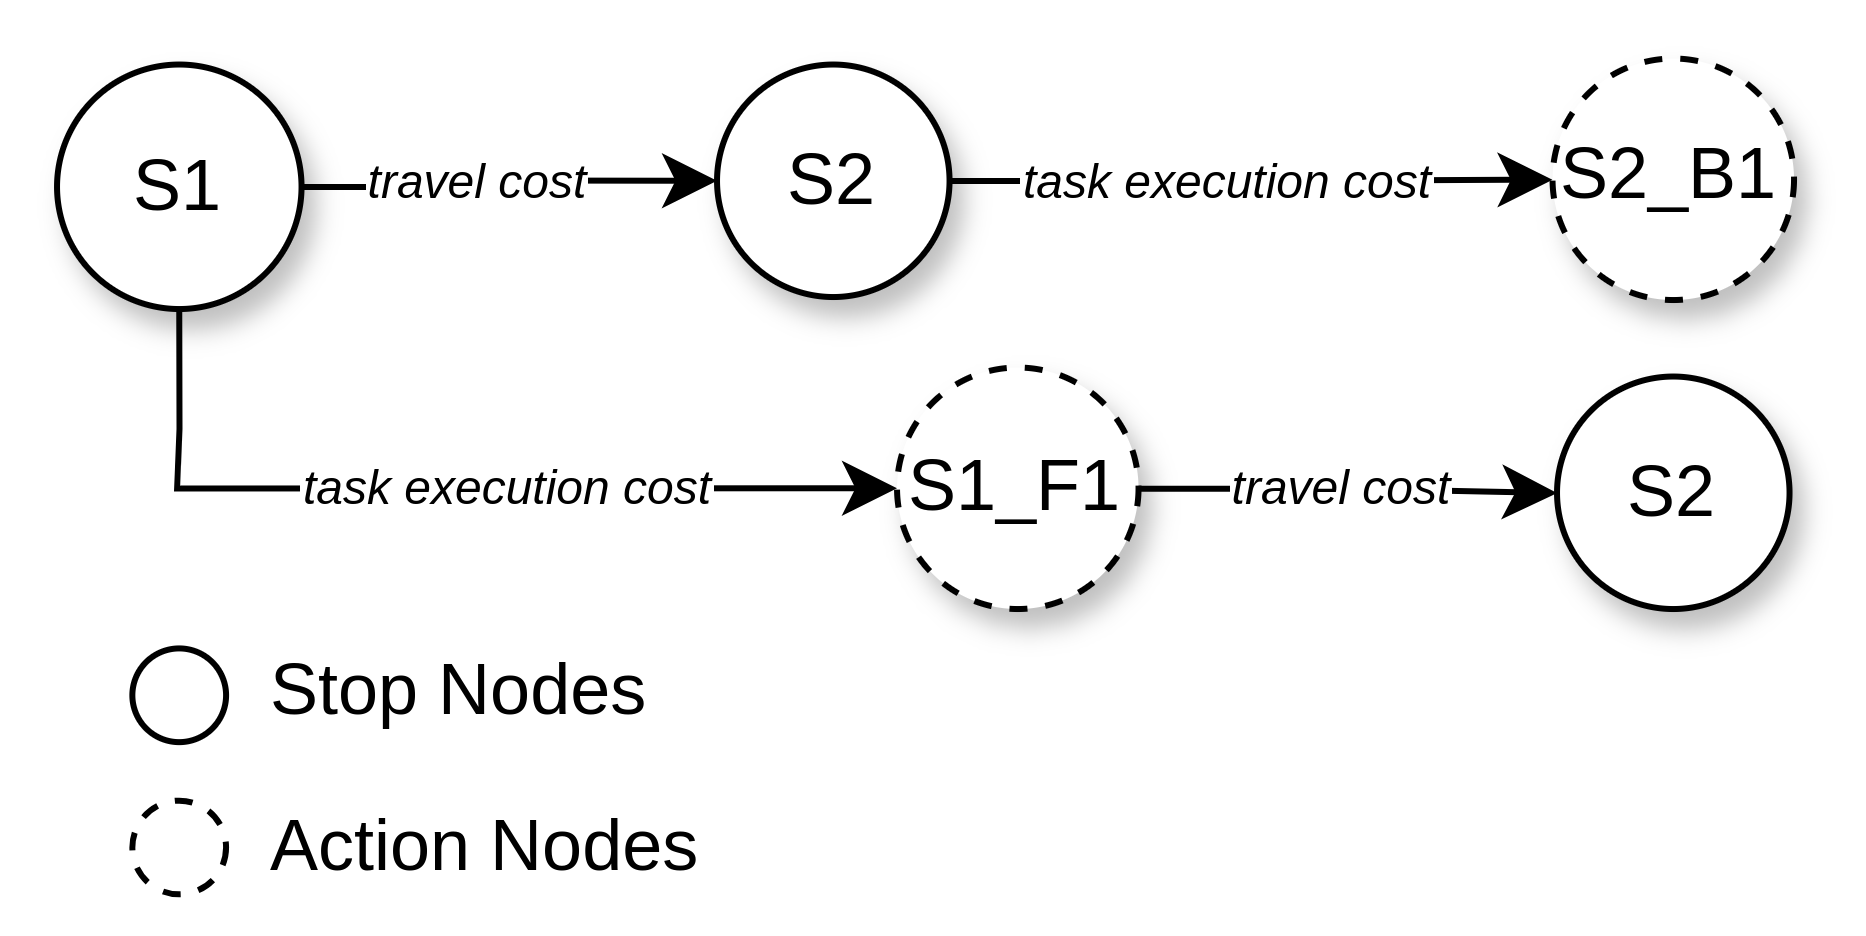
\includegraphics[width=0.8\linewidth]{gfx/ch03/graph_search_nodes.png}
    \caption{Node types and cost representation}
    \label{fig:graph-search-nodes}
\end{figure}

\paragraph{\autoref{fig:graph-search-nodes}} Illustrates the convention used to represent the graph. \texttt{S1} denotes stop number 1, while \texttt{F} or \texttt{B} indicate whether the front or back tool is assigned to remove the weed, followed by the weed ID to be processed. In this example, the task execution cost between \texttt{S1} and \texttt{S1\_F1} would be 45s, as the back tool must wait for the front tool to process 1 plant. The same logic applies to the cost between \texttt{S2} and \texttt{S2\_B1} but for the front tool.

The graph search implementation solution follows the next pipeline:
\begin{enumerate}
    \item Compute \textbf{candidate stops} based on the robot's current position and weed detections. Candidate stops are the locations where an important event ocurs, such as a weed entering or exiting the workspace of a tool.
    \item \textbf{Associate} reachable weeds with candidate stops. This allows the algorithm to determine which weeds can be removed at each stop.
    \item Create a \textbf{graph representation} of the problem using \ac{DFS} algorithm and the convention described in \autoref{fig:graph-search-nodes}. The graph is built by connecting \textit{stop nodes} and \textit{action nodes} using appropriate edge costs, taking into account the predefined associations between stops and tasks.
    \item Get the \textbf{shortest path} in the graph from the root (first stop) to the final node (last stop) using Dijkstra's algorithm.
    \item \textbf{Decode solution} and return the next optimal stop and task allocation as the algorithm's output.
\end{enumerate}

% TODO: Later I could add explanation of step 1 and 2 of the pipeline, candidate stops and association

To build and explore the graph, an implementation of the \ac{DFS} algorithm is used (see Algorithm \ref{alg:dfs}). The \texttt{get\_children\_nodes} method expands the graph by generating child nodes from a given parent node. If the parent node is a \textit{stop node}, it creates child nodes for all valid combinations of reachable tasks that can be processed at that stop. Each combination forms a new child node that reflects the state after removing those tasks (\textit{action node}). Additionally a 'trivial' \textit{stop node} is addded representing the decision to move to the next stop without removing any weeds. On the other hand, if the parent node is an \textit{action node}, this method creates a single \textit{stop node} representing the next stop. Each created edge is added to the graph with a weight based on the associated \textit{task execution cost} or \textit{travel cost}. \autoref{fig:building-graph} illustrates the graph expansion process, where the algorithm grows all possible combinations of tasks at each stop and generates the corresponding child nodes. 

We observe that from \texttt{S3} four possible states can be reached (three \textit{action nodes} and one \textit{stop node}), The transition \texttt{S3\_B1\_F2} achieves zero idle time by optimally balancing tasks between the front and back tools, whereas the other transitions result in higher idle times due to imbalanced assignments. It's important to note that the same stop can be reached through different paths, depending on the actions taken at previous stops. For instance, if task 1 has been removed earlier, it should no longer be considered in subsequent stops. This consideration is crucial when building the graph, as we must ensure that it is expanded only through valid and realistic transitions that reflect feasible execution scenarios.

\begin{figure}[hbt]
    \centering
    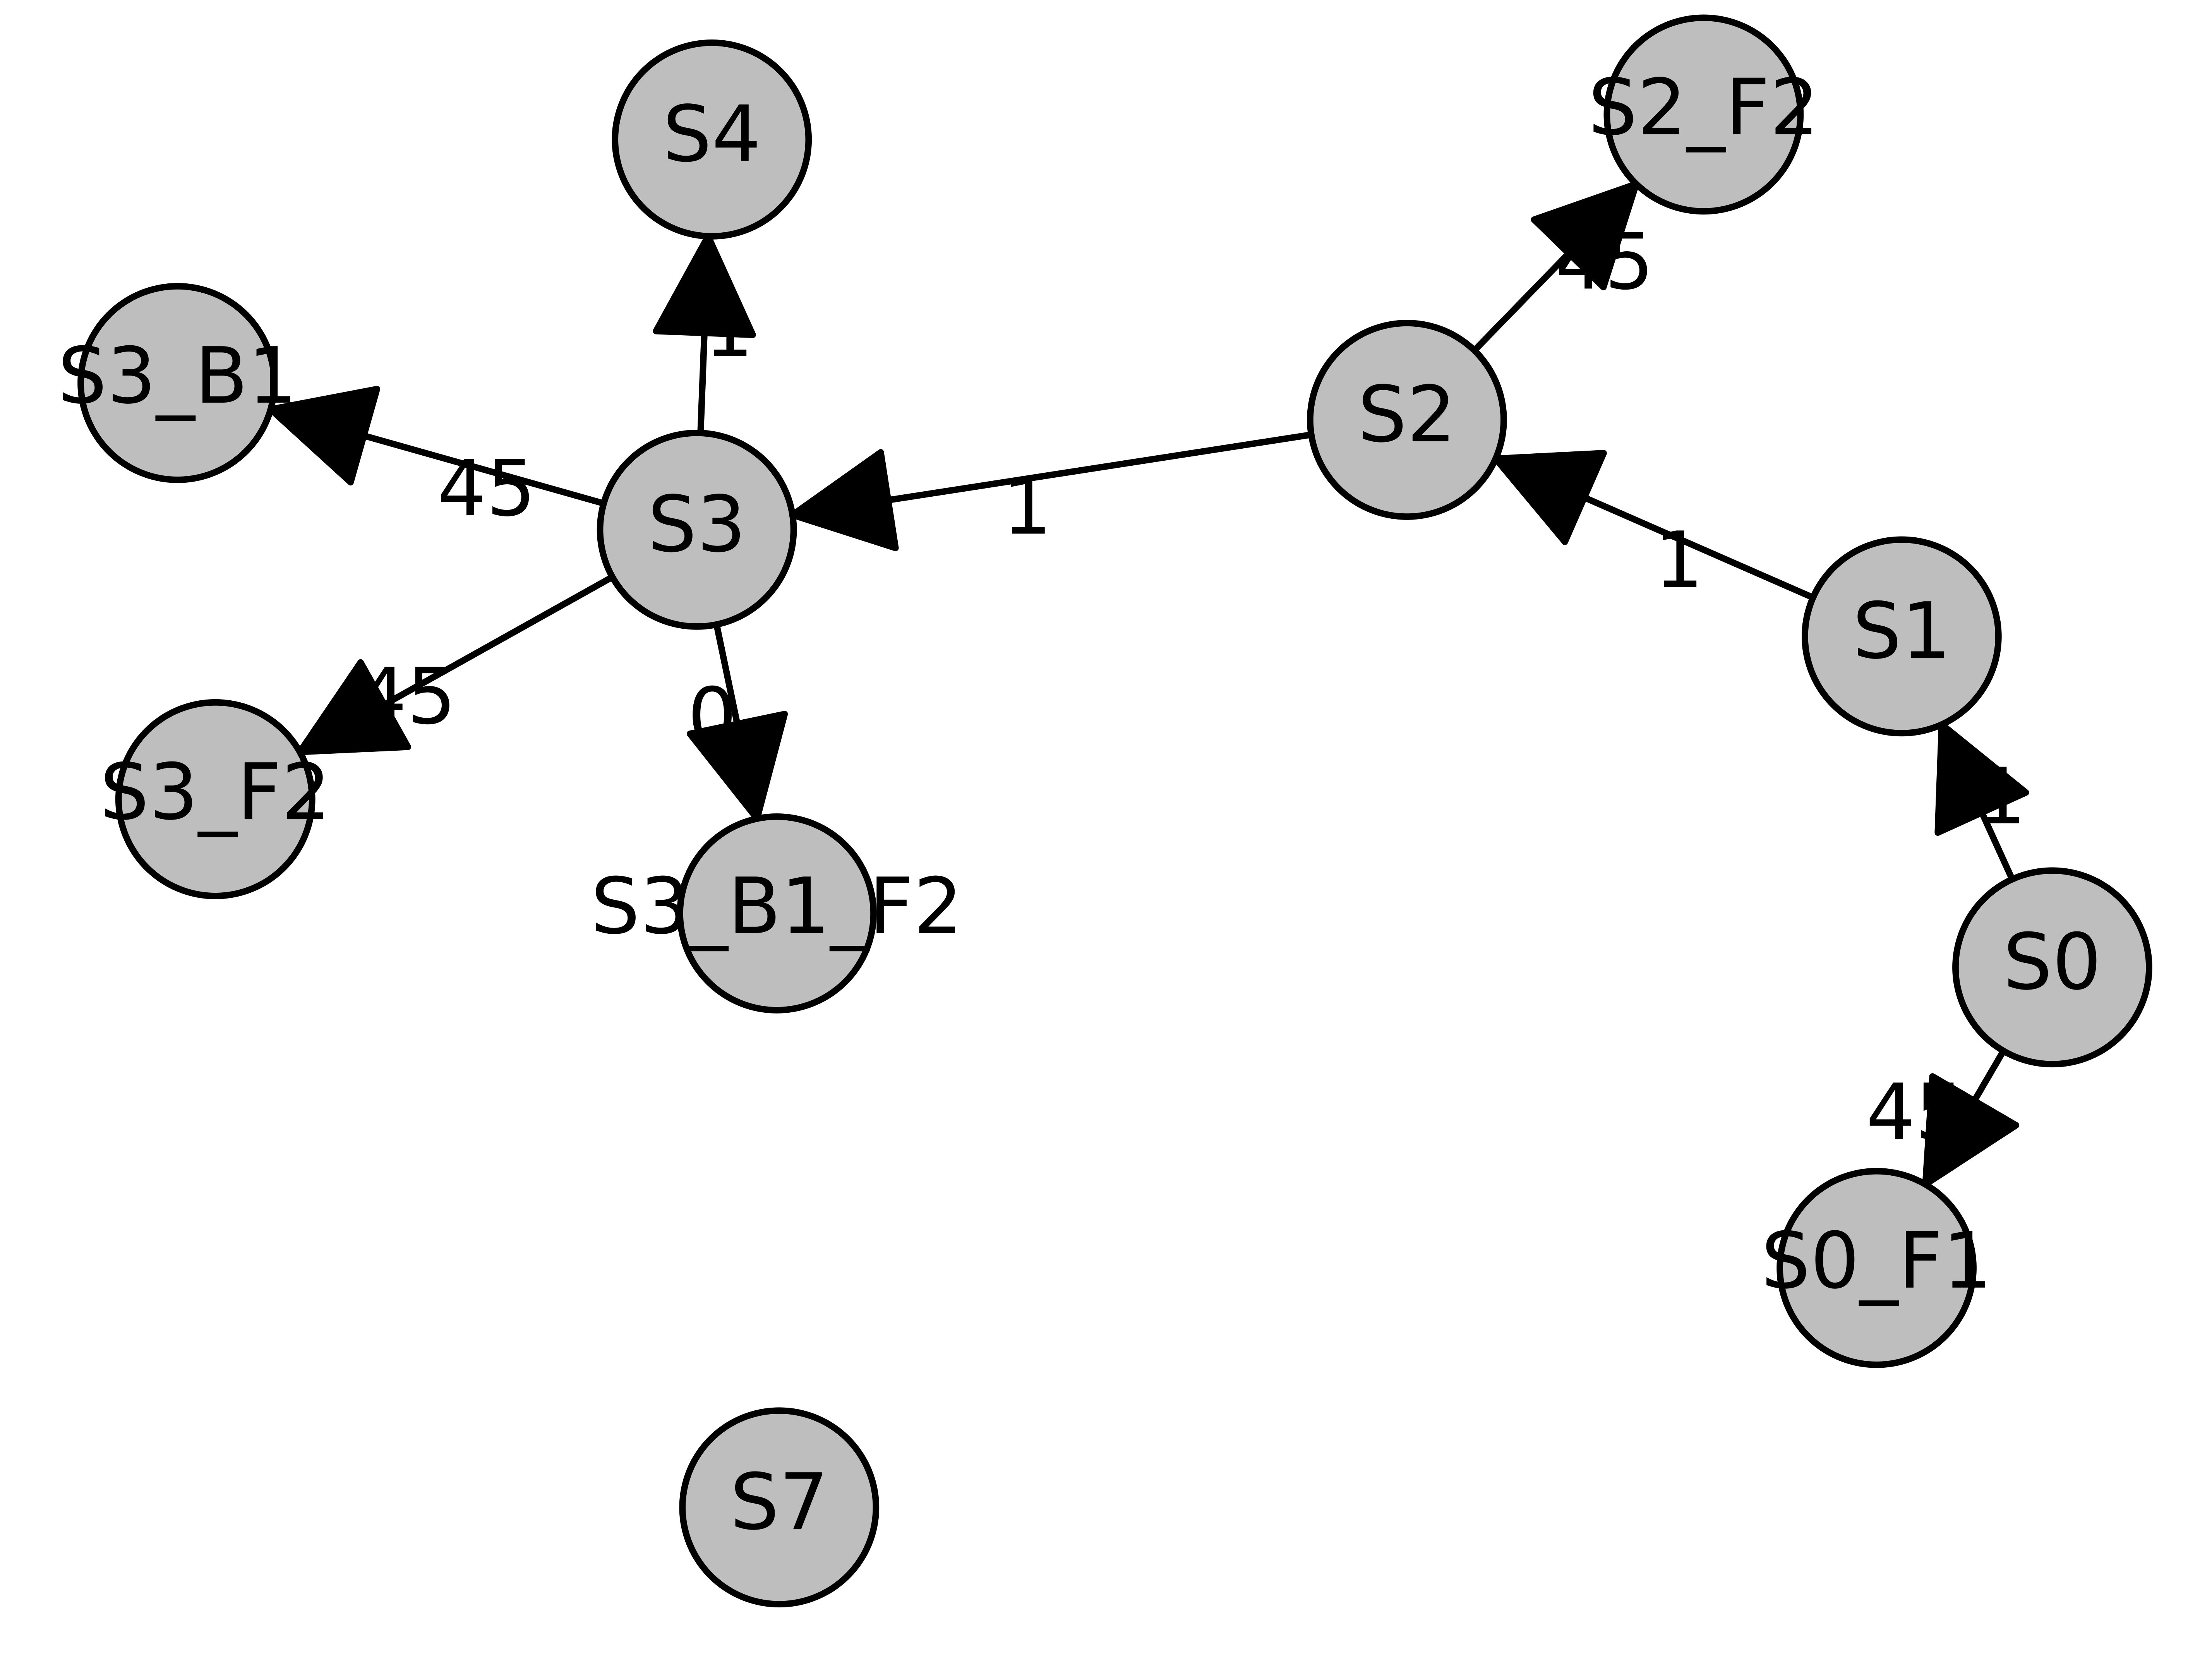
\includegraphics[width=0.7\linewidth]{gfx/ch03/building_graph.png}
    \caption{Graph expansion process}
    \label{fig:building-graph}
\end{figure}

Having the complete graph, and given its configuration as a weighted directed graph, we choose Dijkstra's algorithm to find the optimal path (see Algorihtm \ref{alg:dijkstra}). This algorithm efficiently explores the graph by maintaining a priority queue of nodes to be processed, ensuring that the node with the lowest cost is always explored first. The algorithm continues until it reaches the final node, which represents the optimal solution. The path is then traced back from the final node to the root, revealing the sequence of stops and actions that lead to the optimal solution.

\begin{figure}[htb]
    \myfloatalign
    \subfloat[Path with lowest cost]
    {\label{fig:graph-solution}
        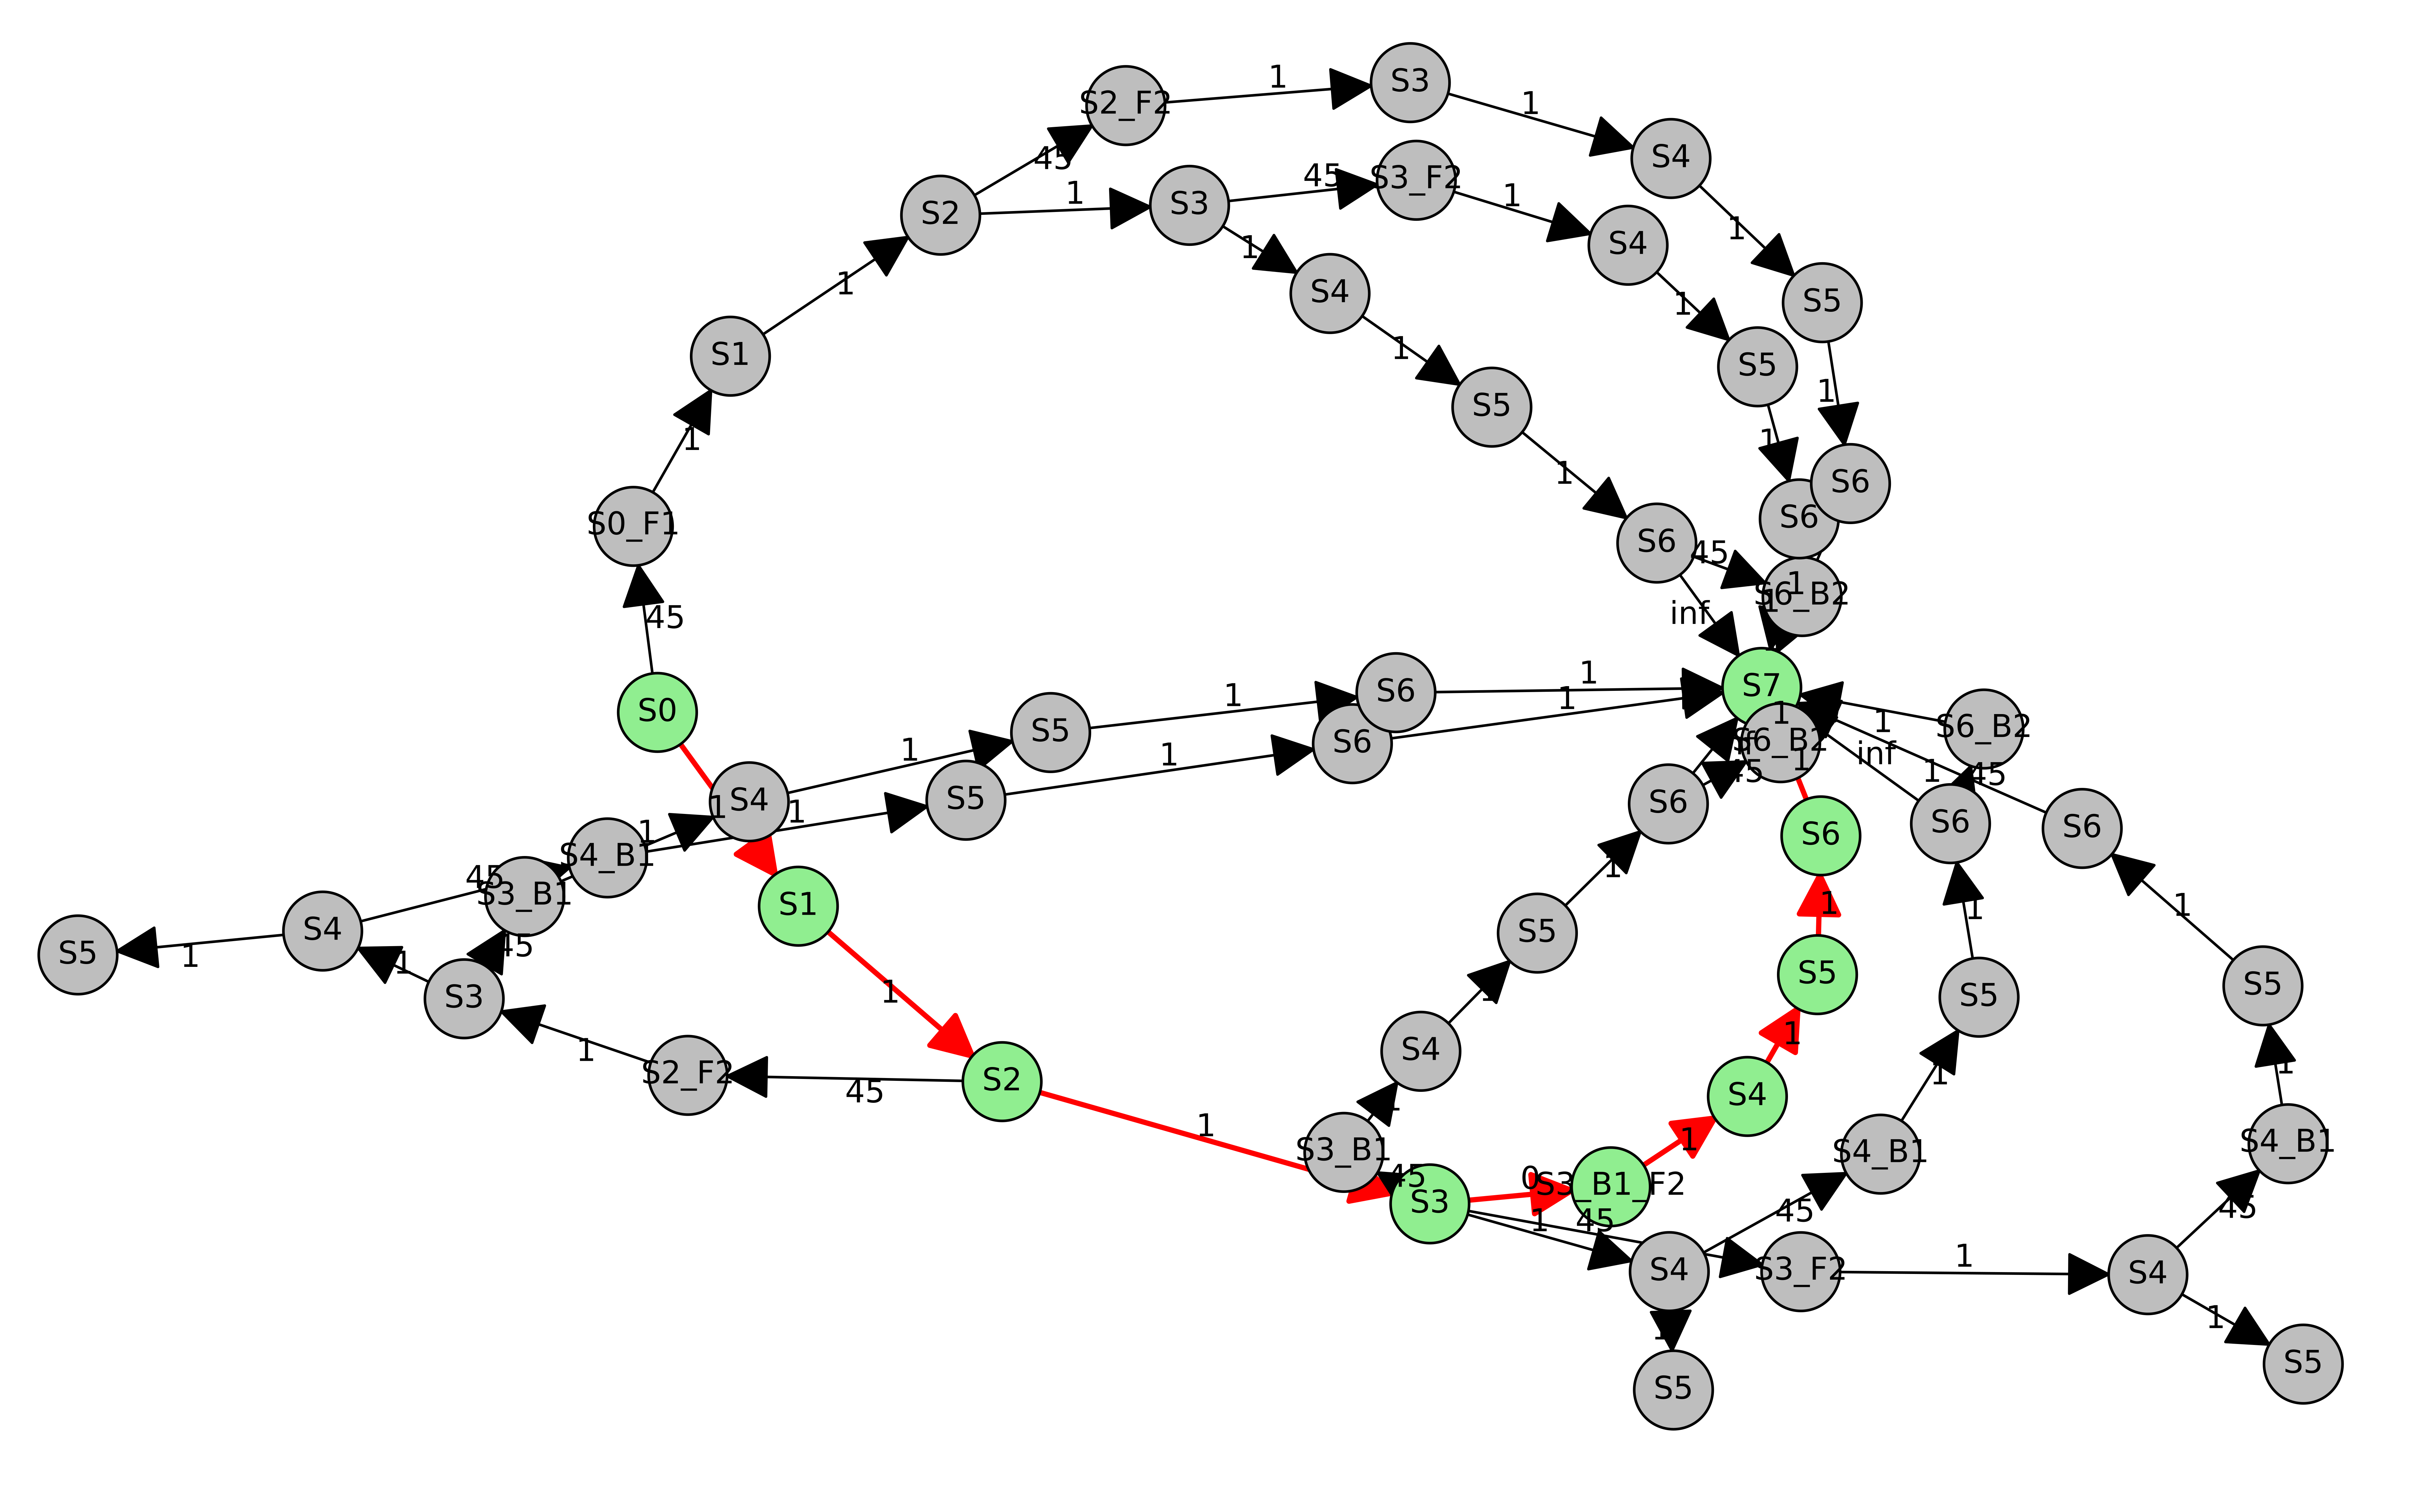
\includegraphics[width=.45\linewidth]{gfx/ch03/graph_solution.png}} \quad
    \subfloat[Task Planning Visualization]
    {\label{fig:scenario-2-tasks}%
        \includegraphics[width=.45\linewidth]{gfx/ch03/scenario_2_tasks.png}} \\
    \caption{Graph Search Solution}\label{fig:graph-search-solution}
\end{figure}

An optimal solution obtained by the graph search algorithm in a scenario with two detected weeds is illustrated in \autoref{fig:graph-solution}. The highlighted branch corresponds to the optimal path found by the algorithm. For the given two weeds, the graph contained 54 nodes, and the computation time was 0.001 seconds. A visual representation of the solution is shown in \autoref{fig:scenario-2-tasks}, including the current robot pose, projected workspaces in red, candidate stops in blue, and weeds in green.

% How we avoid the algorithm chossing trivial solutions where no weeds are removed?
One remaining issue to address is preventing the algorithm from returning trivial solutions in which either no weeds are removed or not all of them are. To tackle this, each node keeps track of the tasks completed so far. If, at the second-to-last node, there are still tasks left to remove, we assign a penalty cost to the edge leading to the final node. This encourages the algorithm to prioritize removing as many weeds as possible before proceeding to the last stop.

Our graph search solution performs well in terms of computation time, for a low to medium density of weeds. However, as the number of weeds increases, the graph size grows exponentially, leading to longer computation times. \autoref{fig:graphsearch-performance} showcases the graph size and computation time for different number of weeds (see plot in red). The graph size is defined as the number of nodes in the graph, while the computation time is the time required to build and find the optimal path in the graph.

\begin{figure}[htb]
    \myfloatalign
    \subfloat[Graph size vs. number of weeds]
    {\label{fig:graphsearch-graph-size}%
        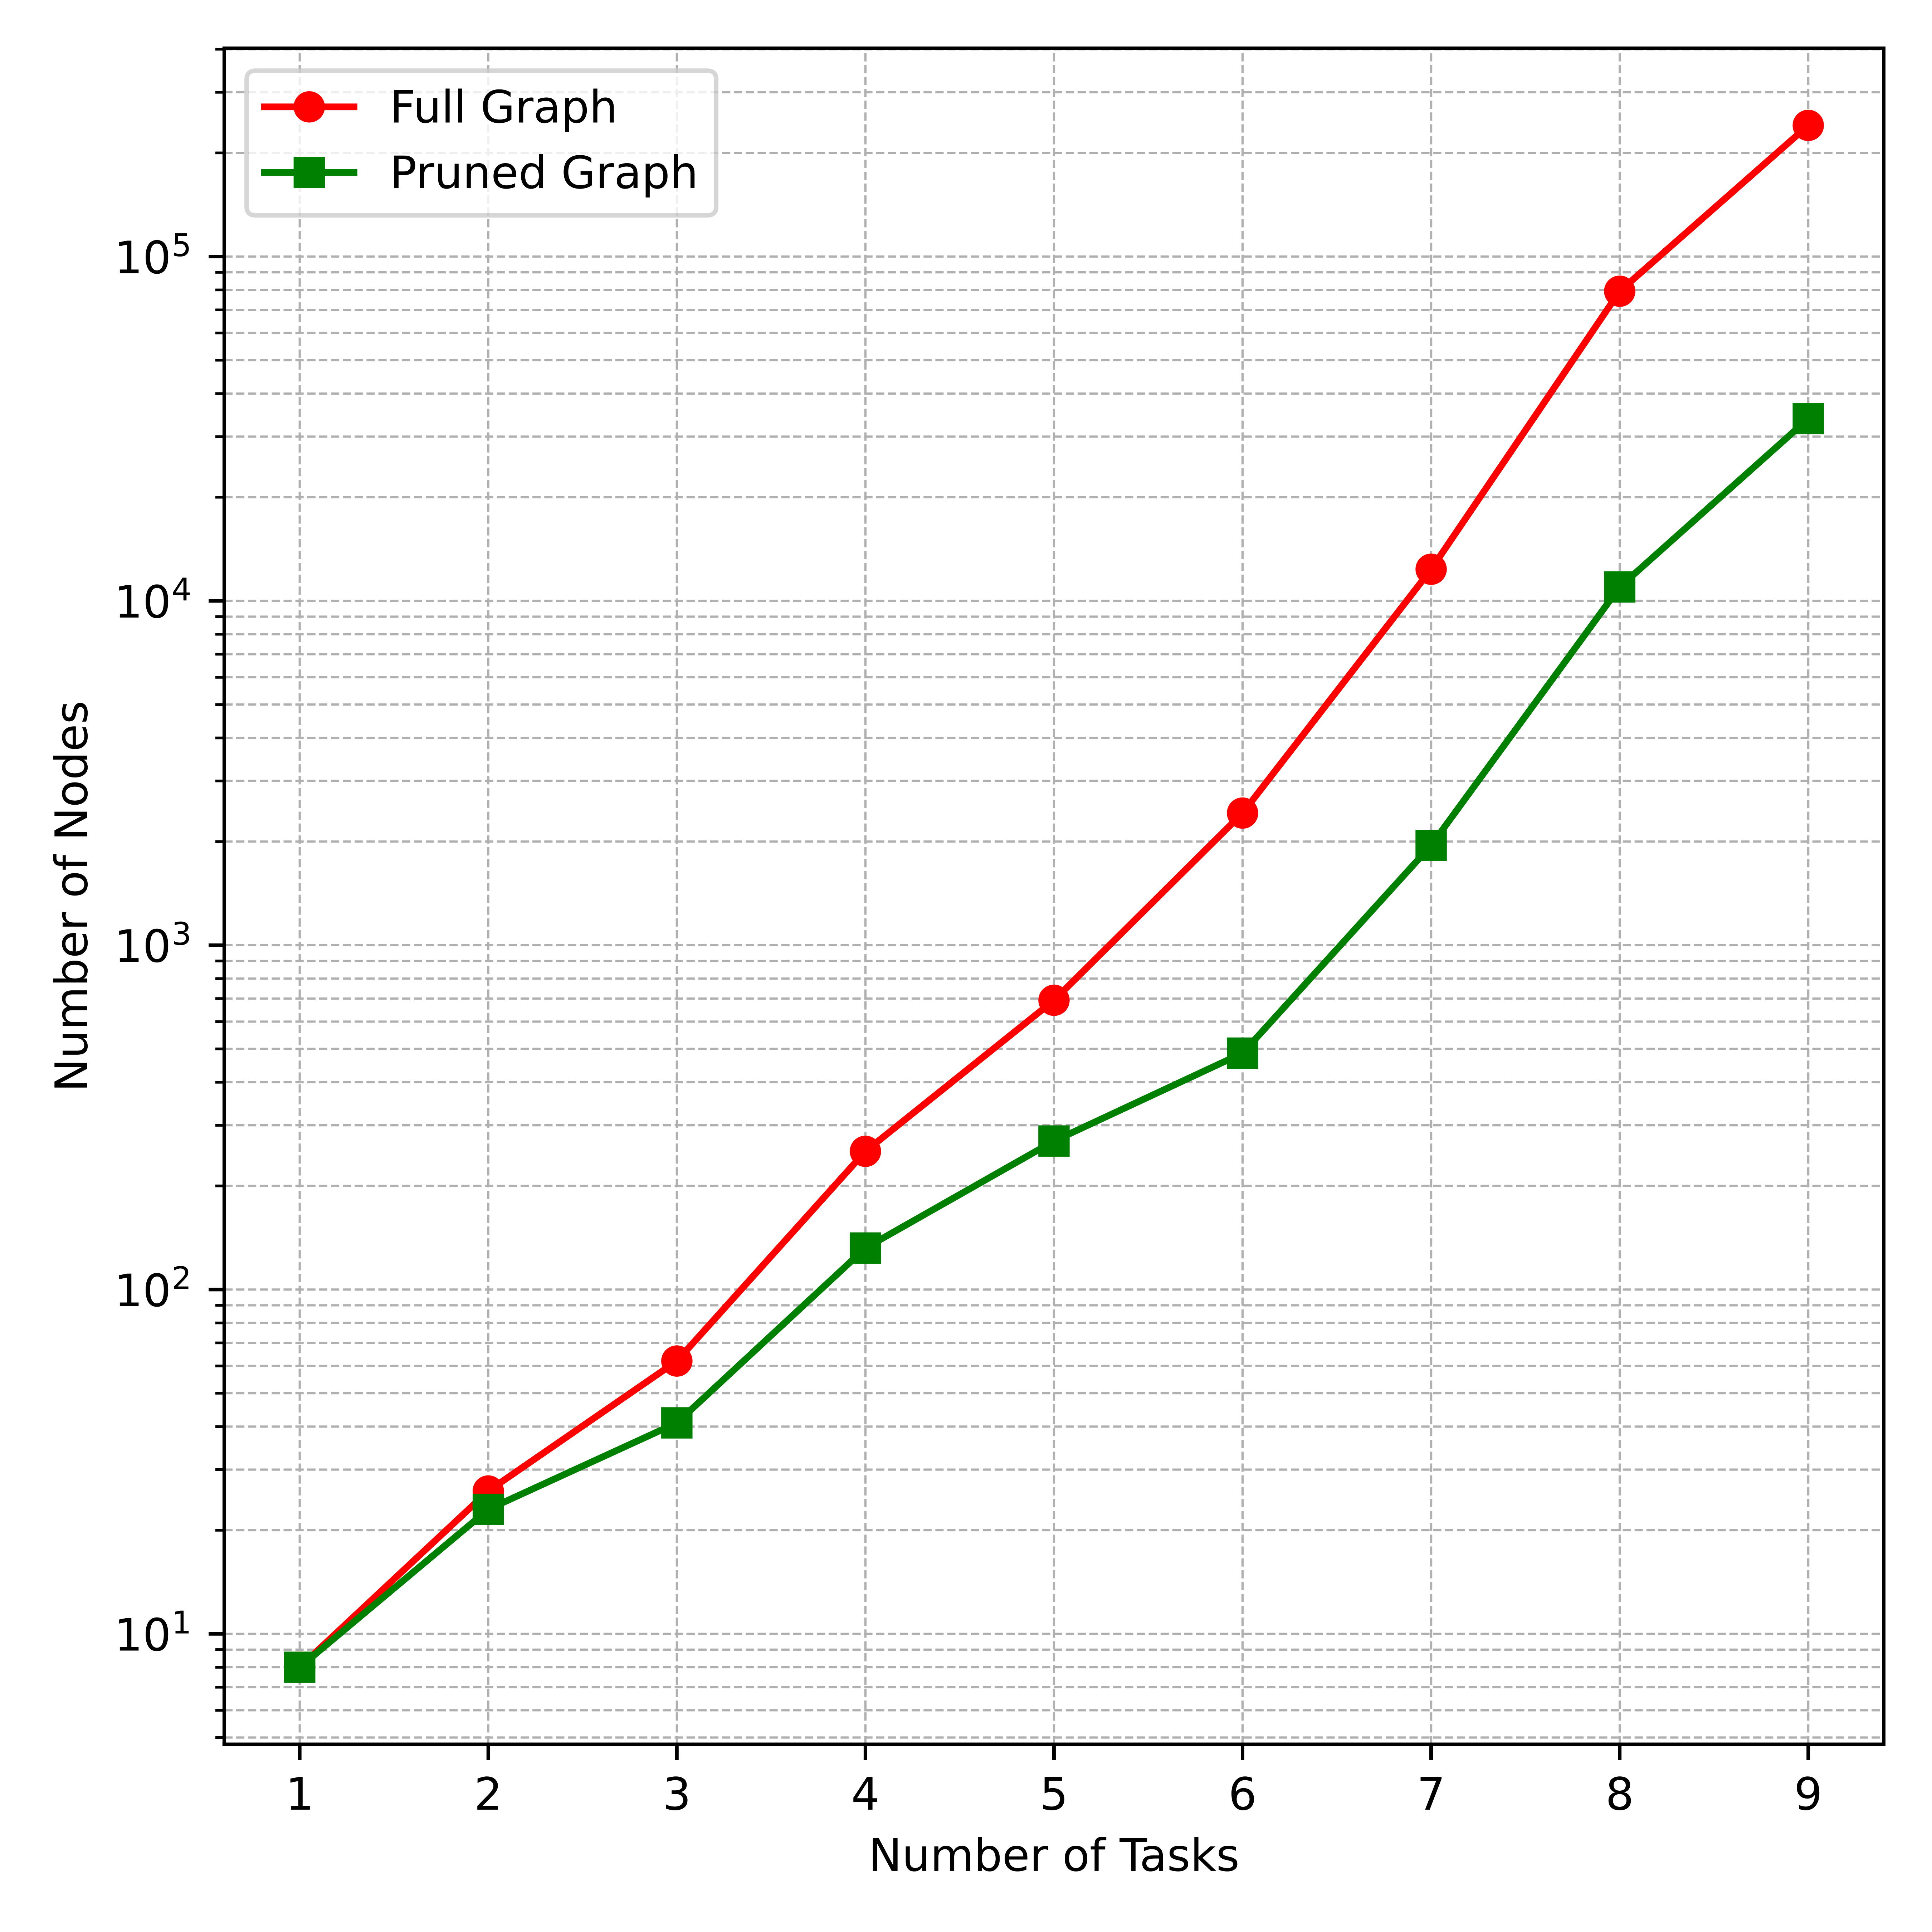
\includegraphics[width=.45\linewidth]{gfx/ch03/gs_graph_size_plot.png}} \quad
    \subfloat[Processing time vs. number of weeds]
    {\label{fig:graphsearch-processing-time}%
        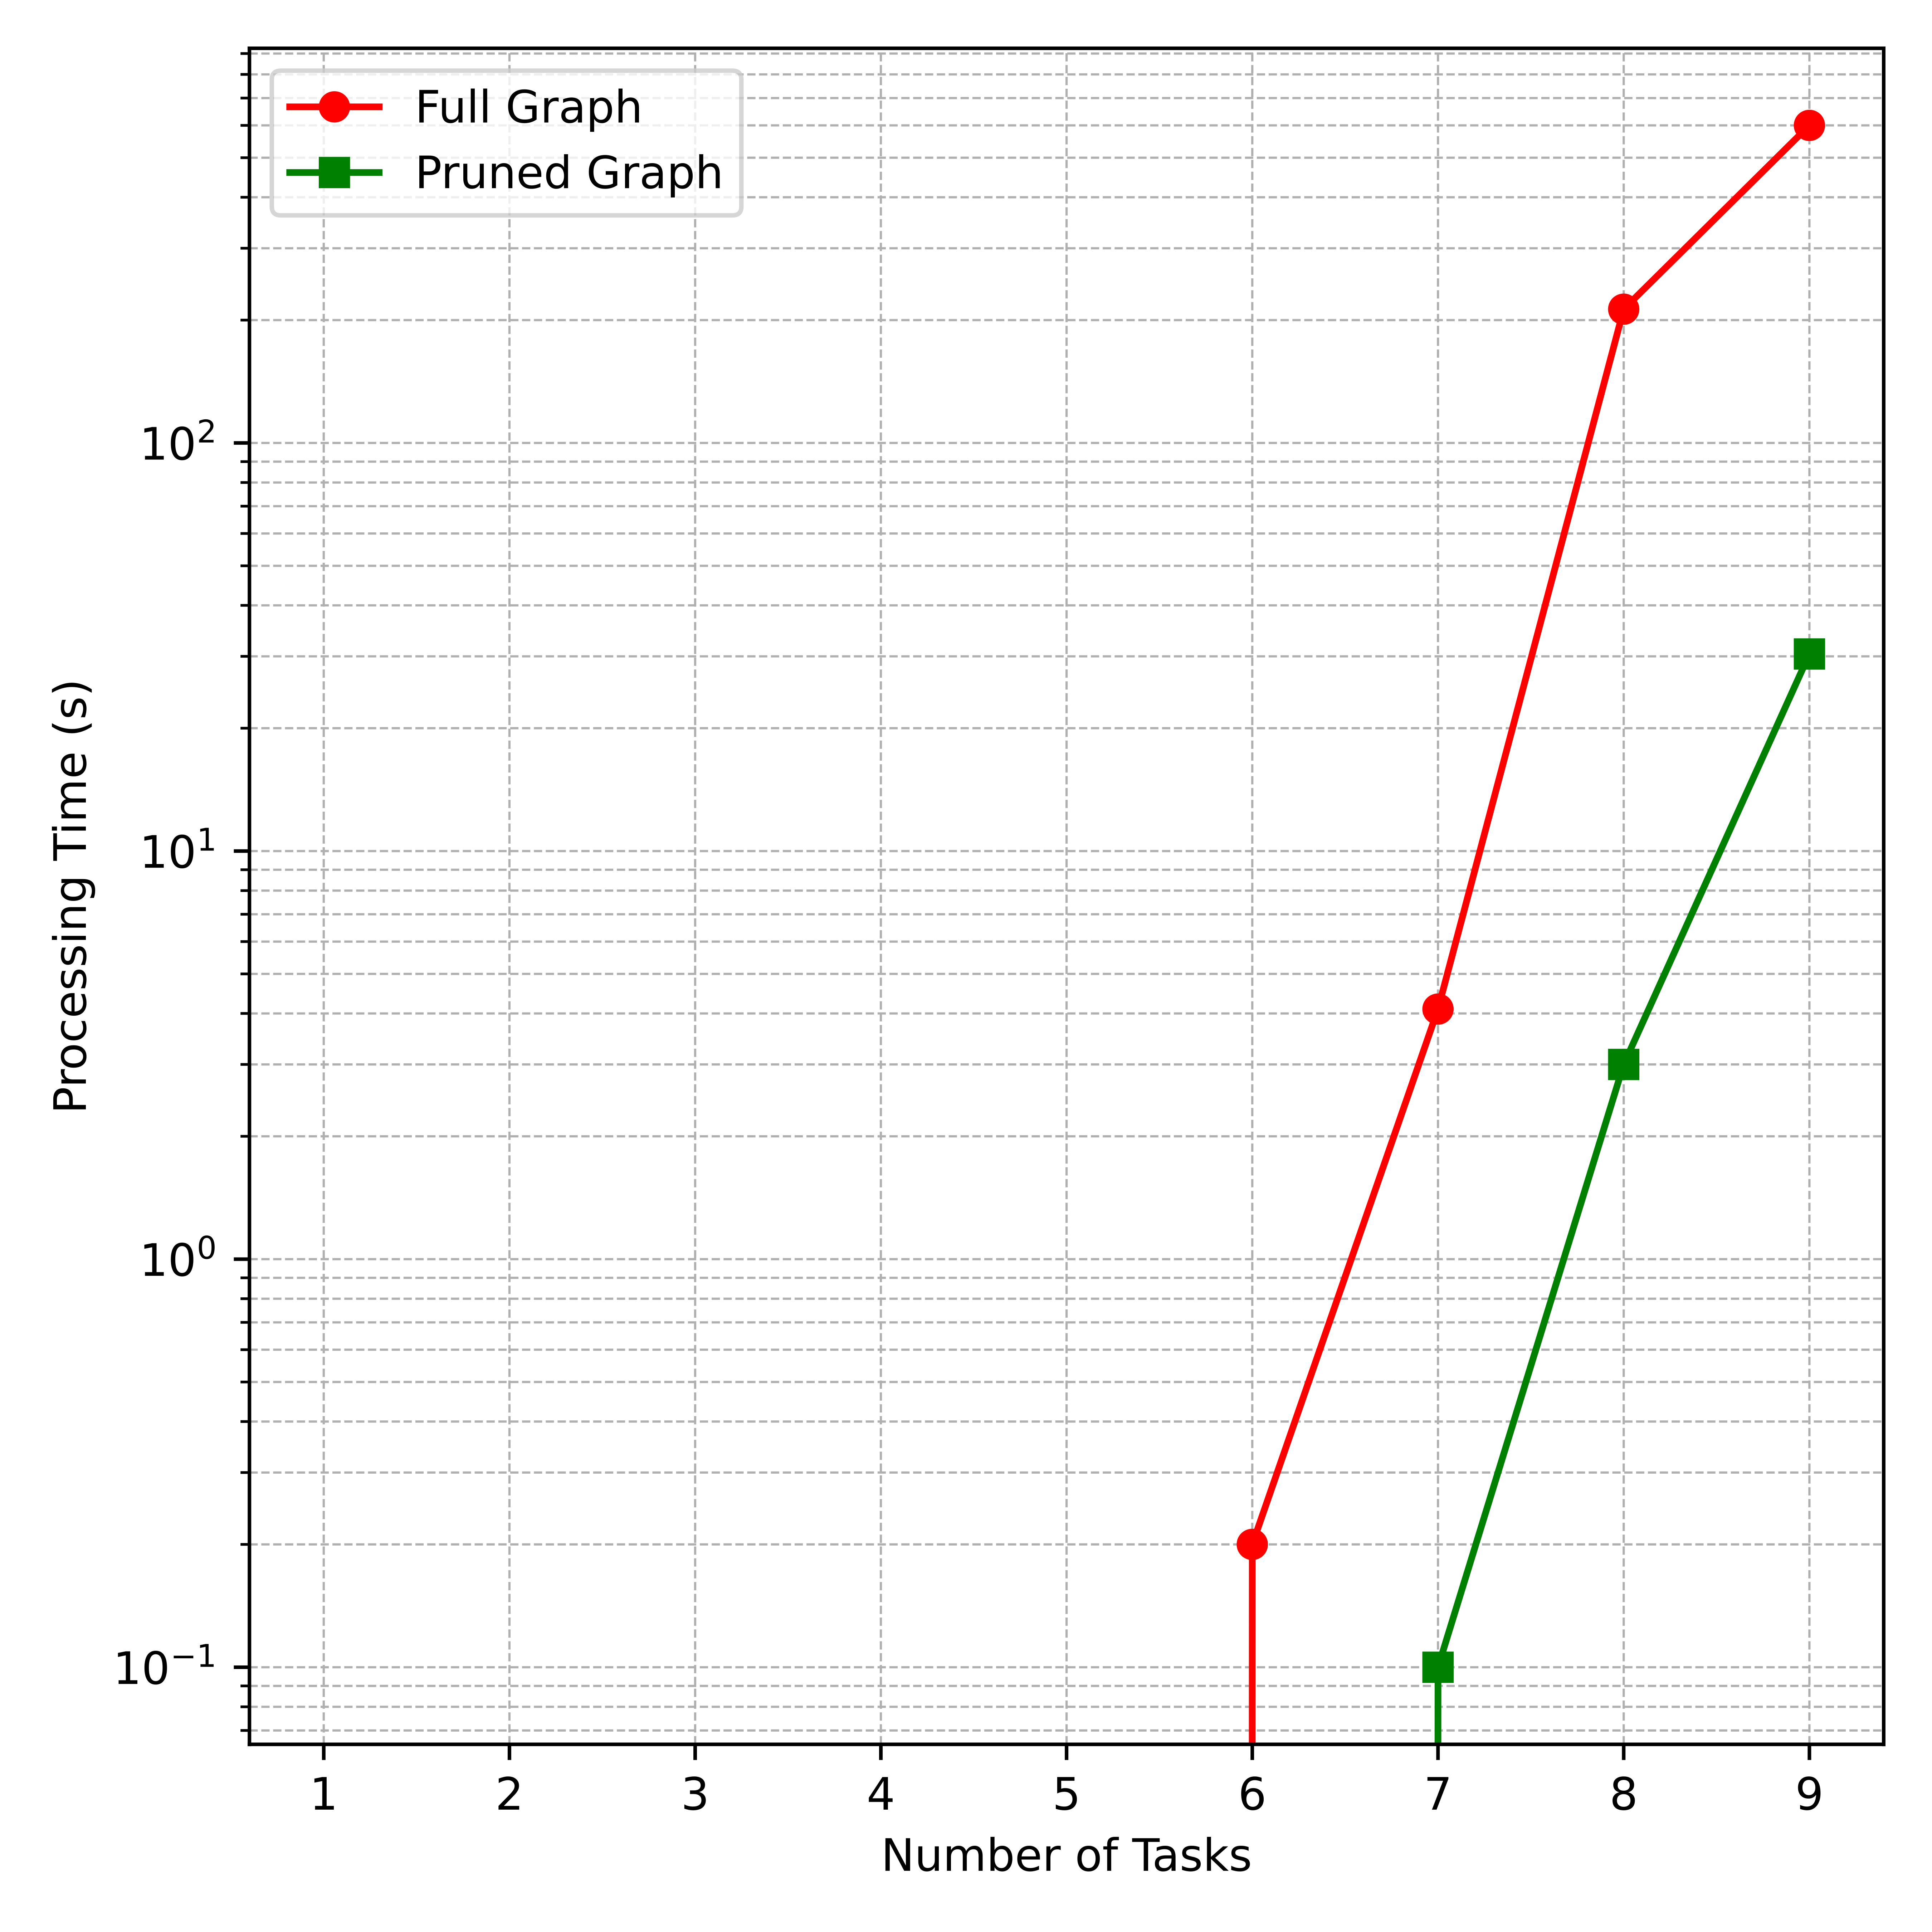
\includegraphics[width=.45\linewidth]{gfx/ch03/gs_proce_time_plot.png}} \\
    \caption{Graph Search algorithm performance}\label{fig:graphsearch-performance}
\end{figure}

We were able to optimize and reduce the graph size by applying a pruning technique that stops the growth of certain branches when they are not promising. This is achieved by introducing the concept of \textit{expired tasks}, these are tasks that haven't been removed and can no longer be removed in future stops because the corresponding weeds have been left behind, outside the tool's workspaces. This pruning is implemented in the \texttt{get\_children\_nodes} method, where each task is checked for expiration before being added to the graph. As a result, the number of nodes is significantly reduced, improving computation time (observe green plot in \autoref{fig:graphsearch-performance}).

Although the graph search algorithm is a promising approach, it still suffers from the exponential growth of the graph size as the number of weeds increases. This can lead to longer computation times and may not be suitable for real-time applications with high weed densities. In the next section, we will explore optimization-based approaches that can potentially overcome these limitations and provide more efficient solutions.

\section{Optimization}
As discussed at the beginning of this chapter, the main goal of \ac{TA} is to find the best allocation of resources and the optimal sequence of stops while considering the given constraints. Achieving such a solution requires mathematically formulating the scenario as an optimization task, with a clearly defined objective function, set of constraints, and decision variables that fully describe the problem. Optimization-based approaches are powerful tools that provide a systematic way to find the best feasible solution to a problem by exproring the solution space. Depending on the nature of the problem, a different optimization formulation can be used, such as linear programming, \ac{MIP}, or nonlinear programming. In our case, we will focus on \ac{MIP} as the most suitable approach for the problem.

\ac{MIP} is a mathematical optimization technique that combines both integer and continuous variables in the formulation of the problem. It allows for the modeling of complex decision-making scenarios where some variables must take on discrete values (e.g., binary decisions) while others can take on continuous values. This flexibility makes \ac{MIP} particularly useful for problems that involve resource allocation, scheduling, and other combinatorial optimization tasks. \\

Given a set of tasks $\mathcal{T} = \{1,2,...,T\}$ where each task $j \in \mathcal{T}$ corresponds to one weed detection from a total $T$, and a set of candidate stops $\mathcal{S} = \{1,2,...,S\}$ where each stop $i \in \mathcal{S}$ is computed using events as in Graph Search algorithm. Let $x_{i,j} \in \{0,1\} $ be a binary decision variable equal to $1$ if task $j$ is assigned to stop $i$, $0$ otherwise and ${imb}_i \in \mathbb{N}_0$ the imbalance of assigned tasks between tools at stop $i$. We know that from each stop $i$ we can only assign tasks that are visible from that stop, and a subset for those corresponds to tasks set to front or back tools, these statements could be better defined as:

\begin{tabular}{ll}
    $\mathcal{V}_i \subseteq \mathcal{T}$ & Set of tasks visible from stop $i$ \\
    $\mathcal{F}_i \subseteq \mathcal{V}_i$ & Front tool task assigned at stop $i$ \\
    $\mathcal{B}_i \subseteq \mathcal{V}_i$ & Back tool task assigned at stop $i$ \\
    $\tau$ & Constant processing time per task \\
\end{tabular}

We know that each task must be assigned to exactly one stop.

\begin{equation}
    \sum_{i=1}^{S} x_{i,j} = 1 \quad \forall j \in \mathcal{T}
\end{equation}

While visible tasks can only be assigned its corresponding stops.

\begin{equation}
    x_{i,j} = 0 \quad \text{if} \quad j \notin \mathcal{V}_i
\end{equation}

The imbalance per stop is the absolute time difference between front and back tools.

\begin{equation}
    f_i = \sum_{j \in \mathcal{F}_i} x_{i,j} \quad \text{and} \quad b_i = \sum_{j \in \mathcal{B}_i} x_{i,j}
\end{equation}

We want the imbalance ${imb}_i$ to reflect the time difference between front and back processing times at each stop. Therefore, we define the imbalance as the maximum of the two possible differences.

\begin{equation}
    \left| \tau (f_i - b_i) \right| = \max \left( f_i - b_i, b_i - f_i \right)
\end{equation}

Thus

\begin{equation}
    {imb}_i \geq \tau \left(f_i - b_i\right) \quad \text{and} \quad {imb}_i \geq \tau \left(b_i - f_i\right)
\end{equation}

Or equivalently

\begin{equation}
    {imb}_i \geq \left| \tau (f_i - b_i) \right| \quad \forall i \in \mathcal{S}
\end{equation}

The objective function is to minimize the total idle time, expressed as follows

\begin{equation}
    \min \sum_{i=1}^{S} {imb}_i
\end{equation}

Given the constraints and objective function, we can formulate the optimization problem as follows:

\begin{equation}
    \begin{aligned}
        \text{minimize} & \quad \sum_{i=1}^{S} {imb}_i \\
        \text{subject to} & \quad \sum_{i=1}^{S} x_{i,j} = 1 \quad \forall j \in \mathcal{T} \\
                          & \quad x_{i,j} = 0 \quad \text{if} \quad j \notin \mathcal{V}_i
    \end{aligned}
\end{equation}

An advantage of an optimization-based approach is that once the problem is formulated we can use existing optimization libraries to obtain the solution. In our case, we used the \texttt{Google OR-Tools}\footnote{OR-Tools is an open source software suite for optimization, tuned for tackling the world's toughest problems in vehicle routing, flows, integer, linear, and constraint programming. \url{https://developers.google.com/optimization}} library to solve our combinatorial problem.

The pipeline for the optimization-based approach is as follows:
\begin{enumerate}
    \item Compute \textbf{candidate stops} based on the robot's current position and weed detections.
    \item \textbf{Associate} reachable weeds with candidate stops.
    \item Build the \textbf{optimization model} using decision variables, constraints, and objective function.
    \item \textbf{Call solver} to get solution.
    \item \textbf{Decode solution} and return the next optimal stop and task allocation as the algorithm's output.
\end{enumerate}

This method does not suffer from high processing times as weed density increases. The algorithm consistently returns a solution in less than 0.1 seconds across a range of weed densities, from low to extremely high (tested up to $6.25$ weeds/m²), making it a strong candidate for real-time applications. The optimization model effectively balances tasks between tools while minimizing idle time. \autoref{fig:mip-solution} illustrates an example of the solution generated by the optimization algorithm in a scenario with twenty weeds.

\begin{figure}[htb]
    \myfloatalign
    \subfloat[Optimization Output]
    {\label{fig:mip-algorithm-output}
        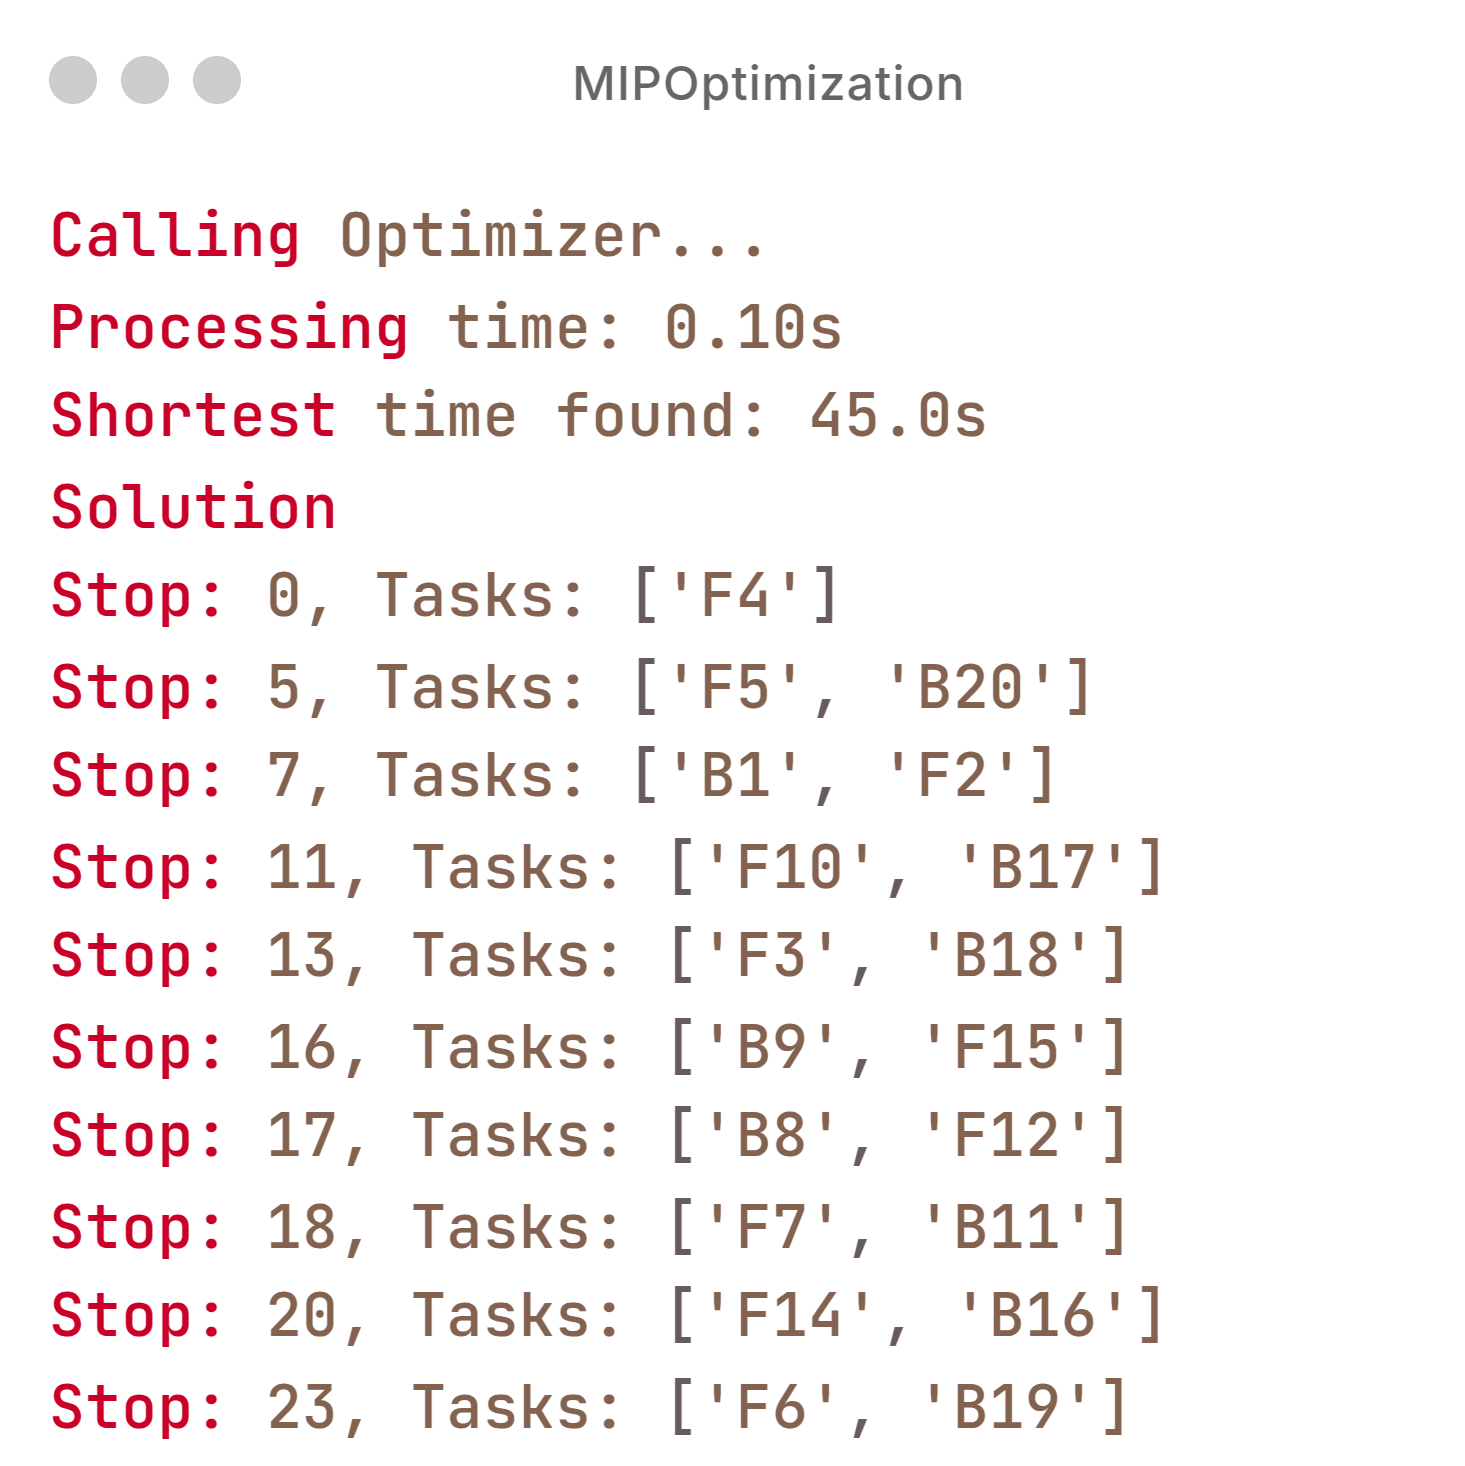
\includegraphics[width=.35\linewidth]{gfx/ch03/mip_solution.png}} \quad
    \subfloat[Task Planning Visualization]
    {\label{fig:mip-scenario-10-tasks}%
        \includegraphics[width=.55\linewidth]{gfx/ch03/mip_scenario_20tasks.png}} \\
    \caption{Mixed-Integer Programming}\label{fig:mip-solution}
\end{figure}

\section{Market-based}
\lipsum[1]

%*****************************************
%*****************************************
%*****************************************
%*****************************************
%*****************************************

%\include{multiToC} % <--- just debug stuff, ignore for your documents
\cleardoublepage%************************************************
\chapter{Conclusions}\label{ch:conclusions}
%************************************************

%*****************************************
%*****************************************
%*****************************************
%*****************************************
%*****************************************
% ********************************************************************
% Backmatter
%*******************************************************
\appendix
%\renewcommand{\thechapter}{\alph{chapter}}
\cleardoublepage
% \part{Appendix}
%********************************************************************
% Appendix
%*******************************************************
% If problems with the headers: get headings in appendix etc. right
%\markboth{\spacedlowsmallcaps{Appendix}}{\spacedlowsmallcaps{Appendix}}
\chapter{Appendix}\label{sec:appendix}
\section{Configuration Files}

\begin{lstlisting}[language=yaml, frame=tb, caption={Weed Infestation World config example}, label={lst:world-yaml}, float=h]
    seed: 2
    quadrant_size: [2.0, 2.0]
    quadrants:
      1:
        direction: x
        weed_density: 0.4   # weeds/m2
        spatial_distribution: clustered
        std_dev: [0.5, 0.5]
        outside_workspace: false
      2:
        direction: x
        weed_density: 1.2   # weeds/m2
        spatial_distribution: uniform
        outside_workspace: false
\end{lstlisting}

\begin{lstlisting}[language=yaml, frame=tb, caption={ROS$2$ config example}, label={lst:ros2_control-yaml}, float=htb]
  # ROS2 Control
  controller_manager:
    ros__parameters:
      use_sim_time: True
      update_rate: 20 # Hz
  
      joint_state_broadcaster:
        type: joint_state_broadcaster/JointStateBroadcaster
  
      forward_position_controller_front:
        type: forward_command_controller/ForwardCommandController
  forward_position_controller_front:
    ros__parameters:
      joints:
        - front_x_axis_joint
        - front_y_axis_joint
        - front_implement_tool_joint
      interface_name: position
\end{lstlisting}

\clearpage
\section{Algorithms}

\begin{algorithm}[H]
  \caption{Depth-First Search}
  \label{alg:dfs}
  \begin{algorithmic}[1]
    \REQUIRE $root\_node$, $last\_node$
    \ENSURE Explored Graph

    \STATE $\text{visited} \gets \{\text{last\_node}\}$ \COMMENT{Initialize with last node}
    \STATE $\text{stack} \gets [\text{root\_node}]$ \COMMENT{Start with root node}
    \STATE $i \gets 0$ \COMMENT{Iteration counter}

    \WHILE{stack is not empty}
    \STATE $i \gets i + 1$
    \STATE $\text{node} \gets \text{stack.pop}()$
    \IF{node $\notin$ visited}
    \STATE $\text{visited.add(node)}$
    \STATE $\text{children} \gets \text{get\_children\_nodes(node)}$

    \IF{children $\neq$ None}
    \STATE $\text{stack.extend(children)}$ \COMMENT{Add children to stack}
    \ENDIF
    \ENDIF
    \IF{$i == 5000$}
    \STATE \textbf{break} \COMMENT{Early termination}
    \ENDIF
    \ENDWHILE
  \end{algorithmic}
\end{algorithm}

\begin{algorithm}[H]
  \caption{Get Next Stop}
  \label{alg:get-next-stop}
  \begin{algorithmic}[1]
    \REQUIRE Detections, Robot pose
    \ENSURE Next stop pose and assigned tasks

    \IF{$\texttt{stop\_pose} \neq \texttt{None}$}
    \STATE \textbf{return}
    \ENDIF

    \IF{\texttt{detections} is empty}
    \STATE $\texttt{nuga\_state} \gets \texttt{"moving"}$
    \STATE \textbf{return}
    \ENDIF

    \STATE $(\texttt{tasks\_in}, \texttt{tasks\_out}) \gets \texttt{get\_tasks\_in\_future\_path()}$
    \STATE $\texttt{now} \gets \texttt{current time}$

    \IF{\texttt{tasks\_out} is not empty}
    \FORALL{$(\texttt{idx}, \texttt{pose}) \in \texttt{tasks\_out}$}
    \STATE $\texttt{tasks\_out\_ws[idx]} \gets \texttt{pose}$
    \STATE \texttt{add\_marker("map", now, "out", idx, pose, "orange")}
    \ENDFOR
    \ENDIF

    \IF{\texttt{tasks\_in} is empty}
    \STATE $\texttt{nuga\_state} \gets \texttt{"moving"}$
    \STATE \textbf{return}
    \ENDIF

    \STATE \texttt{algorithm.set\_robot\_pose(nuga\_pose)}
    \STATE \texttt{algorithm.set\_tasks(tasks\_in)}
    \STATE $(\texttt{stop\_pose}, \texttt{stop\_tasks}) \gets \texttt{algorithm.compute\_next\_stop()}$
    \STATE \texttt{add\_marker("map", now, "goal", stops\_counter + 1, stop\_pose, "blue")}

    \STATE \texttt{clear\_polygons()}
    \STATE $id \gets 0$
    \FORALL{$(\texttt{name}, \texttt{imp}) \in \texttt{implements}$}
    \STATE \texttt{add\_polygon("map", now, name + "\_ws", id, imp.future\_ws\_pose)}
    \STATE $id \gets id + 1$
    \ENDFOR
  \end{algorithmic}
\end{algorithm}

%Ei solet nemore consectetuer nam. Ad eam porro impetus, te choro omnes
%evertitur mel. Molestie conclusionemque vel at, no qui omittam
%expetenda efficiendi. Eu quo nobis offendit, verterem scriptorem ne
%vix.


%********************************************************************
% Other Stuff in the Back
%*******************************************************
\pdfbookmark[-1]{Back Matter}{back} % Dummy part bookmark for back matter
\cleardoublepage%********************************************************************
% Bibliography
%*******************************************************
% work-around to have small caps also here in the headline
% https://tex.stackexchange.com/questions/188126/wrong-header-in-bibliography-classicthesis
% Thanks to Enrico Gregorio
\defbibheading{bibintoc}[\bibname]{%
  \phantomsection
  \manualmark
  \markboth{\spacedlowsmallcaps{#1}}{\spacedlowsmallcaps{#1}}%
  \addtocontents{toc}{\protect\vspace{\beforebibskip}}%
  \addcontentsline{toc}{chapter}{#1}%
  % \addcontentsline{toc}{chapter}{\tocEntry{#1}}%
  \chapter*{#1}%
}
\printbibliography[heading=bibintoc]

% Old version, will be removed later
% work-around to have small caps also here in the headline
%\manualmark
%\markboth{\spacedlowsmallcaps{\bibname}}{\spacedlowsmallcaps{\bibname}} % work-around to have small caps also
%\phantomsection
%\refstepcounter{dummy}
%\addtocontents{toc}{\protect\vspace{\beforebibskip}} % to have the bib a bit from the rest in the toc
%\addcontentsline{toc}{chapter}{\tocEntry{\bibname}}
%\label{app:bibliography}
%\printbibliography

% \cleardoublepage%*******************************************************
% Declaration
%*******************************************************
\pdfbookmark[0]{Declaration}{declaration}
\chapter*{Declaration}
\thispagestyle{empty}
Put your declaration here.
\bigskip

\noindent\textit{\myLocation, \myTime}

\smallskip

\begin{flushright}
    \begin{tabular}{m{5cm}}
        \\ \hline
        \centering\myName \\
    \end{tabular}
\end{flushright}

% \cleardoublepage\pagestyle{empty}

\hfill

\vfill


\pdfbookmark[0]{Colophon}{colophon}
\section*{Colophon}
This document was typeset using the typographical look-and-feel \texttt{classicthesis} developed by Andr\'e Miede and Ivo Pletikosić.
The style was inspired by Robert Bringhurst's seminal book on typography ``\emph{The Elements of Typographic Style}''.
\texttt{classicthesis} is available for both \LaTeX\ and \mLyX:
\begin{center}
\url{https://bitbucket.org/amiede/classicthesis/}
\end{center}
Happy users of \texttt{classicthesis} usually send a real postcard to the author, a collection of postcards received so far is featured here:
\begin{center}
\url{http://postcards.miede.de/}
\end{center}
Thank you very much for your feedback and contribution.

\bigskip

\noindent\finalVersionString

%Hermann Zapf's \emph{Palatino} and \emph{Euler} type faces (Type~1 PostScript fonts \emph{URW
%Palladio L} and \emph{FPL}) are used. The ``typewriter'' text is typeset in \emph{Bera Mono},
%originally developed by Bitstream, Inc. as ``Bitstream Vera''. (Type~1 PostScript fonts were made
%available by Malte Rosenau and
%Ulrich Dirr.)

%\paragraph{note:} The custom size of the textblock was calculated
%using the directions given by Mr. Bringhurst (pages 26--29 and
%175/176). 10~pt Palatino needs  133.21~pt for the string
%``abcdefghijklmnopqrstuvwxyz''. This yields a good line length between
%24--26~pc (288--312~pt). Using a ``\emph{double square textblock}''
%with a 1:2 ratio this results in a textblock of 312:624~pt (which
%includes the headline in this design). A good alternative would be the
%``\emph{golden section textblock}'' with a ratio of 1:1.62, here
%312:505.44~pt. For comparison, \texttt{DIV9} of the \texttt{typearea}
%package results in a line length of 389~pt (32.4~pc), which is by far
%too long. However, this information will only be of interest for
%hardcore pseudo-typographers like me.%
%
%To make your own calculations, use the following commands and look up
%the corresponding lengths in the book:
%\begin{verbatim}
%    \settowidth{\abcd}{abcdefghijklmnopqrstuvwxyz}
%    \the\abcd\ % prints the value of the length
%\end{verbatim}
%Please see the file \texttt{classicthesis.sty} for some precalculated
%values for Palatino and Minion.
%
%    \settowidth{\abcd}{abcdefghijklmnopqrstuvwxyz}
%    \the\abcd\ % prints the value of the length

% ********************************************************************
% Game Over: Restore, Restart, or Quit?
%*******************************************************
\end{document}
% ********************************************************************
